

%---------------------------------------------------------------------------------------
%	PACKAGES AND OTHER DOCUMENT CONFIGURATIONS
%----------------------------------------------------------------------------------------

\documentclass[11pt,fleqn]{book} % Default font size and left-justified equations

%%%%%%%%%%%%%%%%%%%%%%%%%%%%%%%%%%%%%%%%%
% The Legrand Orange Book
% Structural Definitions File
% Version 2.0 (9/2/15)
%
% Original author:
% Mathias Legrand (legrand.mathias@gmail.com) with modifications by:
% Vel (vel@latextemplates.com) and Andrey Kravtsov (akravtsov@gmail.com)
% 
% This file has been downloaded from:
% http://www.LaTeXTemplates.com
%
% License:
% CC BY-NC-SA 3.0 (http://creativecommons.org/licenses/by-nc-sa/3.0/)
%
%%%%%%%%%%%%%%%%%%%%%%%%%%%%%%%%%%%%%%%%%%%%%%%%%%%%%%%%%%%%%%%%%%%%%%%%%%%%%%%%%%
% The Legrand Orange Book
% LaTeX Template
% Version 2.1.1 (14/2/16)
%
% This template has been downloaded from:
% http://www.LaTeXTemplates.com
%
% Original author:
% Mathias Legrand (legrand.mathias@gmail.com) with modifications by:
% Vel (vel@latextemplates.com)
%
% License:
% CC BY-NC-SA 3.0 (http://creativecommons.org/licenses/by-nc-sa/3.0/)
%
% Compiling this template:
% This template uses biber for its bibliography and makeindex for its index.
% When you first open the template, compile it from the command line with the 
% commands below to make sure your LaTeX distribution is configured correctly:
%
% 1) pdflatex main
% 2) makeindex main.idx -s StyleInd.ist
% 3) biber main
% 4) pdflatex main x 2
%
% After this, when you wish to update the bibliography/index use the appropriate
% command above and make sure to compile with pdflatex several times 
% afterwards to propagate your changes to the document.
%
% This template also uses a number of packages which may need to be
% updated to the newest versions for the template to compile. It is strongly
% recommended you update your LaTeX distribution if you have any
% compilation errors.
%
% Important note:
% Chapter heading images should have a 2:1 width:height ratio,
% e.g. 920px width and 460px height.
%
%%%%%%%%%%%%%%%%%%%%%%%%%%%%%%%%%%%%%%%%%
%----------------------------------------------------------------------------------------
%	VARIOUS REQUIRED PACKAGES AND CONFIGURATIONS
%----------------------------------------------------------------------------------------

\usepackage[top=3cm,bottom=3cm,left=3cm,right=3cm,headsep=10pt,a4paper]{geometry} % Page margins

\usepackage{graphicx} % Required for including pictures
\usepackage{amsmath}
\usepackage{hyperref}      
\usepackage{mathptmx}
\usepackage{anyfontsize}
\usepackage{t1enc}

\graphicspath{{fig/}} % Specifies the directory where pictures are stored

\usepackage{lipsum} % Inserts dummy text

\usepackage{tikz} % Required for drawing custom shapes

\usepackage[english]{babel} % English language/hyphenation

\usepackage{enumitem} % Customize lists
\setlist{nolistsep} % Reduce spacing between bullet points and numbered lists

\usepackage{booktabs} % Required for nicer horizontal rules in tables

\usepackage{xcolor} % Required for specifying colors by name
%\definecolor{ocre}{RGB}{243,102,25} % Define the orange color used for highlighting throughout the book
\definecolor{ocre}{RGB}{119,181,254} % Define the orange color used for highlighting throughout the book

\usepackage{listings}
\usepackage{color}

\definecolor{dkgreen}{rgb}{0,0.6,0}
\definecolor{gray}{rgb}{0.5,0.5,0.5}
\definecolor{mauve}{rgb}{0.58,0,0.82}

\lstset{frame=tb,
  language=Java,
  aboveskip=3mm,
  belowskip=3mm,
  showstringspaces=false,
  columns=flexible,
  basicstyle={\small\ttfamily},
  numbers=none,
  numberstyle=\tiny\color{gray},
  keywordstyle=\color{blue},
  commentstyle=\color{dkgreen},
  stringstyle=\color{mauve},
  breaklines=true,
  breakatwhitespace=true,
  tabsize=3
}

\usepackage{fancyhdr}
\usepackage{graphicx}
%\usepackage{references}
%\usepackage{natbib209}
\pagestyle{fancy}
\headheight 35pt 
\setlength{\textwidth}{6.5in}
\setlength{\textheight}{9.5in}
\setlength{\topmargin}{-0.75in}
\setlength{\headheight}{1.0cm}
\setlength{\headwidth}{\textwidth}
\setlength{\headsep}{0.5cm}
\setlength{\oddsidemargin}{0in}
\setlength{\evensidemargin}{0in}
\setlength{\footskip}{0.7cm}

\def\textfraction{0.07}
\def\floatpagefraction{0.93}

\fancyhead{}
\fancyfoot{}
%\lhead[{\sffamily{\bfseries\thepage}%
%                   \hfill Simulations of structure formation}]{}
\lhead[{\sffamily{\bfseries\thepage}}%
                   \hfill {\sffamily\nouppercase{\rightmark}}]{}
\rhead[]{\sffamily\nouppercase{\leftmark}%
                   \hfill {\bfseries\thepage}}
%\citestyle{aa}

% redefine vector command
\renewcommand{\vec}[1]{{\boldsymbol{#1}}}

%------------------------------
% some shorthand definitions
%-----------------------------

\def\Msun{\rm M_{\odot}}
\def\hMsun{h^{-1}\rm\,M_{\odot}}
\def\Mvir{M_{\rm vir}}
\def\Np{N_{\rm p}}
\def\Lbox{L_{\rm box}}
\def\Vbox{V_{\rm box}}
\def\kNy{k_{\rm Ny}}

\def\dim#1{\mbox{\,#1}}

\def\subem{m}
\def\subbe{b}
\def\Om{\Omega_\subem}
\def\Ob{\Omega_\subbe}
\def\Ol{\Omega_\Lambda}
\def\Ok{\Omega_K}
\def\Or{\Omega_R}

\def\aeq{a_{\rm eq}}

\def\imath{{\mathsf i}}


\def\refjnl#1{{\rmfamily#1}}%
\newcommand\aj{\refjnl{AJ}}%
          % Astronomical Journal
\newcommand\araa{\refjnl{ARA\&A}}%
          % Annual Review of Astron and Astrophys
\newcommand\apj{\refjnl{ApJ}}%
          % Astrophysical Journal
\newcommand\apjl{\refjnl{ApJ}}%
          % Astrophysical Journal, Letters
\newcommand\apjs{\refjnl{ApJS}}%
          % Astrophysical Journal, Supplement
\newcommand\apss{\refjnl{Ap\&SS}}%
          % Astrophysics and Space Science
\newcommand\aap{\refjnl{A\&A}}%
          % Astronomy and Astrophysics
\newcommand\aapr{\refjnl{A\&A~Rev.}}%
          % Astronomy and Astrophysics Reviews
\newcommand\azh{\refjnl{AZh}}%
          % Astronomicheskii Zhurnal
\newcommand\mnras{\refjnl{MNRAS}}%
          % Monthly Notices of the RAS
\newcommand\na{\refjnl{New A}}%
  % New Astronomy
\newcommand\nar{\refjnl{New A Rev.}}%
  % New Astronomy Review
\newcommand\pra{\refjnl{Phys.~Rev.~A}}%
          % Physical Review A: General Physics
\newcommand\prb{\refjnl{Phys.~Rev.~B}}%
          % Physical Review B: Solid State
\newcommand\prc{\refjnl{Phys.~Rev.~C}}%
          % Physical Review C
\newcommand\prd{\refjnl{Phys.~Rev.~D}}%
          % Physical Review D
\newcommand\pre{\refjnl{Phys.~Rev.~E}}%
          % Physical Review E
\newcommand\prl{\refjnl{Phys.~Rev.~Lett.}}%
          % Physical Review Letters
\newcommand\pasp{\refjnl{PASP}}%
          % Publications of the ASP
\newcommand\pasj{\refjnl{PASJ}}%
          % Publications of the ASJ
\newcommand\pasa{\refjnl{PASA}}%
          % Publications of the ASA
\newcommand\sovast{\refjnl{Soviet~Ast.}}%
          % Soviet Astronomy
\newcommand\ssr{\refjnl{Space~Sci.~Rev.}}%
          % Space Science Reviews
\newcommand\nat{\refjnl{Nature}}%
          % Nature
\newcommand\jcp{\refjnl{J.~Comp.~Phys.}}%
          % Journal of Computational Physics


% code names
\def\P3M{P$^3$M}

%\def\grtsim {\lower .1ex\hbox{\rlap{\raise .6ex\hbox{\hskip .3ex
%       {\ifmmode{\scriptscriptstyle >}\else
%                {$\scriptscriptstyle >$}\fi}}}
%        \kern -.4ex{\ifmmode{\scriptscriptstyle \sim}\else
%                {$\scriptscriptstyle\sim$}\fi}}}
%\def\lesssim {\lower .1ex\hbox{\rlap{\raise .6ex\hbox{\hskip .3ex
%        {\ifmmode{\scriptscriptstyle <}\else
%                {$\scriptscriptstyle <$}\fi}}}
%        \kern -.4ex{\ifmmode{\scriptscriptstyle \sim}\else
%                {$\scriptscriptstyle\sim$}\fi}}}


\usepackage{wrapfig} 
\usepackage{framed}
%\usepackage{color}
%\definecolor{shadecolor}{gray}{0.0}


\def\toolbox#1#2{\wrapfloat{minipage}{#1}{#2}\begin{framed}}
\def\endtoolbox{\end{framed}\endwrapfloat}

%
%  Implementing pseudo-code snippets
%
\def\fname#1{{\bf #1}}
\def\fcall#1#2#3{{\fname{#1}{\tt [In:#2;Out:#3]}}}
\def\algorithm#1#2#3{\begin{leftbar}{\tt procedure \fcall{#1}{#2}{#3}}\sl\begin{enumerate}}
\def\endalgorithm{\end{enumerate}\end{leftbar}}


%\def\citet#1{\note{Author names go here}\cite{#1}}
%\def\citep#1{\cite{#1}}



%----------------------------------------------------------------------------------------
%	FONTS
%----------------------------------------------------------------------------------------

\usepackage{avant} % Use the Avantgarde font for headings
%\usepackage{times} % Use the Times font for headings
\usepackage{mathptmx} % Use the Adobe Times Roman as the default text font together with math symbols from the Sym­bol, Chancery and Com­puter Modern fonts

\usepackage{microtype} % Slightly tweak font spacing for aesthetics
\usepackage[utf8]{inputenc} % Required for including letters with accents
\usepackage[T1]{fontenc} % Use 8-bit encoding that has 256 glyphs

%----------------------------------------------------------------------------------------
%	BIBLIOGRAPHY AND INDEX
%----------------------------------------------------------------------------------------

%\usepackage[citestyle=authoryear,style=alphabetic,natbib=true,sorting=nyt,sortcites=true,autopunct=true,babel=hyphen,hyperref=true,abbreviate=false,backref=true,backend=biber]{biblatex}
\usepackage[backend=bibtex,style=authoryear,sortcites=true,autopunct=true,babel=hyphen,hyperref=true,abbreviate=false,backref=false,natbib]{biblatex}
%\usepackage{natbib}
%\newcommand{\citep}{\autocite}
%\newcommand{\citet}{\textcite}
%\newcommand{\citealp}{\cite}
\addbibresource{galaxies.bib} % BibTeX bibliography file
%\defbibheading{bibempty}{}

\usepackage{calc} % For simpler calculation - used for spacing the index letter headings correctly
\usepackage{makeidx} % Required to make an index
\makeindex % Tells LaTeX to create the files required for indexing

%----------------------------------------------------------------------------------------
%	MAIN TABLE OF CONTENTS
%----------------------------------------------------------------------------------------

\usepackage{titletoc} % Required for manipulating the table of contents

\contentsmargin{0cm} % Removes the default margin

% Part text styling
\titlecontents{part}[0cm]
{\addvspace{20pt}\centering\large\bfseries}
{}
{}
{}

% Chapter text styling
\titlecontents{chapter}[1.25cm] % Indentation
{\addvspace{12pt}\large\sffamily\bfseries} % Spacing and font options for chapters
{\color{ocre!60}\contentslabel[\Large\thecontentslabel]{1.25cm}\color{ocre}} % Chapter number
{\color{ocre}}  
{\color{ocre!60}\normalsize\;\titlerule*[.5pc]{.}\;\thecontentspage} % Page number

% Section text styling
\titlecontents{section}[1.25cm] % Indentation
{\addvspace{3pt}\sffamily\bfseries} % Spacing and font options for sections
{\contentslabel[\thecontentslabel]{1.25cm}} % Section number
{}
{\hfill\color{black}\thecontentspage} % Page number
[]

% Subsection text styling
\titlecontents{subsection}[1.25cm] % Indentation
{\addvspace{1pt}\sffamily\small} % Spacing and font options for subsections
{\contentslabel[\thecontentslabel]{1.25cm}} % Subsection number
{}
{\ \titlerule*[.5pc]{.}\;\thecontentspage} % Page number
[]

% List of figures
\titlecontents{figure}[0em]
{\addvspace{-5pt}\sffamily}
{\thecontentslabel\hspace*{1em}}
{}
{\ \titlerule*[.5pc]{.}\;\thecontentspage}
[]

% List of tables
\titlecontents{table}[0em]
{\addvspace{-5pt}\sffamily}
{\thecontentslabel\hspace*{1em}}
{}
{\ \titlerule*[.5pc]{.}\;\thecontentspage}
[]

%----------------------------------------------------------------------------------------
%	MINI TABLE OF CONTENTS IN PART HEADS
%----------------------------------------------------------------------------------------

% Chapter text styling
\titlecontents{lchapter}[0em] % Indenting
{\addvspace{15pt}\large\sffamily\bfseries} % Spacing and font options for chapters
{\color{ocre}\contentslabel[\Large\thecontentslabel]{1.25cm}\color{ocre}} % Chapter number
{}  
{\color{ocre}\normalsize\sffamily\bfseries\;\titlerule*[.5pc]{.}\;\thecontentspage} % Page number

% Section text styling
\titlecontents{lsection}[0em] % Indenting
{\sffamily\small} % Spacing and font options for sections
{\contentslabel[\thecontentslabel]{1.25cm}} % Section number
{}
{}

% Subsection text styling
\titlecontents{lsubsection}[.5em] % Indentation
{\normalfont\footnotesize\sffamily} % Font settings
{}
{}
{}

%----------------------------------------------------------------------------------------
%	PAGE HEADERS
%----------------------------------------------------------------------------------------

\usepackage{fancyhdr} % Required for header and footer configuration

\pagestyle{fancy}
\renewcommand{\chaptermark}[1]{\markboth{\sffamily\normalsize\bfseries\chaptername\ \thechapter.\ #1}{}} % Chapter text font settings
\renewcommand{\sectionmark}[1]{\markright{\sffamily\normalsize\thesection\hspace{5pt}#1}{}} % Section text font settings
\fancyhf{} \fancyhead[LE,RO]{\sffamily\normalsize\thepage} % Font setting for the page number in the header
\fancyhead[LO]{\rightmark} % Print the nearest section name on the left side of odd pages
\fancyhead[RE]{\leftmark} % Print the current chapter name on the right side of even pages
\renewcommand{\headrulewidth}{0.5pt} % Width of the rule under the header
\addtolength{\headheight}{2.5pt} % Increase the spacing around the header slightly
\renewcommand{\footrulewidth}{0pt} % Removes the rule in the footer
\fancypagestyle{plain}{\fancyhead{}\renewcommand{\headrulewidth}{0pt}} % Style for when a plain pagestyle is specified

% Removes the header from odd empty pages at the end of chapters
\makeatletter
\renewcommand{\cleardoublepage}{
\clearpage\ifodd\c@page\else
\hbox{}
\vspace*{\fill}
\thispagestyle{empty}
\newpage
\fi}

%----------------------------------------------------------------------------------------
%	THEOREM STYLES
%----------------------------------------------------------------------------------------

\usepackage{amsmath,amsfonts,amssymb,amsthm} % For math equations, theorems, symbols, etc

\newcommand{\intoo}[2]{\mathopen{]}#1\,;#2\mathclose{[}}
\newcommand{\ud}{\mathop{\mathrm{{}d}}\mathopen{}}
\newcommand{\intff}[2]{\mathopen{[}#1\,;#2\mathclose{]}}
\newtheorem{notation}{Notation}[chapter]

% Boxed/framed environments
\newtheoremstyle{ocrenumbox}% % Theorem style name
{0pt}% Space above
{0pt}% Space below
{\normalfont}% % Body font
{}% Indent amount
{\small\bf\sffamily\color{ocre}}% % Theorem head font
{\;}% Punctuation after theorem head
{0.25em}% Space after theorem head
{\small\sffamily\color{ocre}\thmname{#1}\nobreakspace\thmnumber{\@ifnotempty{#1}{}\@upn{#2}}% Theorem text (e.g. Theorem 2.1)
\thmnote{\nobreakspace\the\thm@notefont\sffamily\bfseries\color{black}---\nobreakspace#3.}} % Optional theorem note
\renewcommand{\qedsymbol}{$\blacksquare$}% Optional qed square

\newtheoremstyle{blacknumex}% Theorem style name
{5pt}% Space above
{5pt}% Space below
{\normalfont}% Body font
{} % Indent amount
{\small\bf\sffamily}% Theorem head font
{\;}% Punctuation after theorem head
{0.25em}% Space after theorem head
{\small\sffamily{\tiny\ensuremath{\blacksquare}}\nobreakspace\thmname{#1}\nobreakspace\thmnumber{\@ifnotempty{#1}{}\@upn{#2}}% Theorem text (e.g. Theorem 2.1)
\thmnote{\nobreakspace\the\thm@notefont\sffamily\bfseries---\nobreakspace#3.}}% Optional theorem note

\newtheoremstyle{blacknumbox} % Theorem style name
{0pt}% Space above
{0pt}% Space below
{\normalfont}% Body font
{}% Indent amount
{\small\bf\sffamily}% Theorem head font
{\;}% Punctuation after theorem head
{0.25em}% Space after theorem head
{\small\sffamily\thmname{#1}\nobreakspace\thmnumber{\@ifnotempty{#1}{}\@upn{#2}}% Theorem text (e.g. Theorem 2.1)
\thmnote{\nobreakspace\the\thm@notefont\sffamily\bfseries---\nobreakspace#3.}}% Optional theorem note

% Non-boxed/non-framed environments
\newtheoremstyle{ocrenum}% % Theorem style name
{5pt}% Space above
{5pt}% Space below
{\normalfont}% % Body font
{}% Indent amount
{\small\bf\sffamily\color{ocre}}% % Theorem head font
{\;}% Punctuation after theorem head
{0.25em}% Space after theorem head
{\small\sffamily\color{ocre}\thmname{#1}\nobreakspace\thmnumber{\@ifnotempty{#1}{}\@upn{#2}}% Theorem text (e.g. Theorem 2.1)
\thmnote{\nobreakspace\the\thm@notefont\sffamily\bfseries\color{black}---\nobreakspace#3.}} % Optional theorem note
\renewcommand{\qedsymbol}{$\blacksquare$}% Optional qed square
\makeatother

% Defines the theorem text style for each type of theorem to one of the three styles above
\newcounter{dummy} 
\numberwithin{dummy}{section}
\theoremstyle{ocrenumbox}
\newtheorem{theoremeT}[dummy]{Theorem}
\newtheorem{problem}{Problem}[chapter]
\newtheorem{exerciseT}{Exercise}[chapter]
\theoremstyle{blacknumex}
\newtheorem{exampleT}{Example}[chapter]
\theoremstyle{blacknumbox}
\newtheorem{vocabulary}{Vocabulary}[chapter]
\newtheorem{definitionT}{Definition}[section]
\newtheorem{corollaryT}[dummy]{Corollary}
\theoremstyle{ocrenum}
\newtheorem{proposition}[dummy]{Proposition}

%----------------------------------------------------------------------------------------
%	DEFINITION OF COLORED BOXES
%----------------------------------------------------------------------------------------

\RequirePackage[framemethod=default]{mdframed} % Required for creating the theorem, definition, exercise and corollary boxes

% Theorem box
\newmdenv[skipabove=7pt,
skipbelow=7pt,
backgroundcolor=black!5,
linecolor=ocre,
innerleftmargin=5pt,
innerrightmargin=5pt,
innertopmargin=5pt,
leftmargin=0cm,
rightmargin=0cm,
innerbottommargin=5pt]{tBox}

% Exercise box	  
\newmdenv[skipabove=7pt,
skipbelow=7pt,
rightline=false,
leftline=true,
topline=false,
bottomline=false,
backgroundcolor=ocre!10,
linecolor=ocre,
innerleftmargin=5pt,
innerrightmargin=5pt,
innertopmargin=5pt,
innerbottommargin=5pt,
leftmargin=0cm,
rightmargin=0cm,
linewidth=4pt]{eBox}	

% Definition box
\newmdenv[skipabove=7pt,
skipbelow=7pt,
rightline=false,
leftline=true,
topline=false,
bottomline=false,
linecolor=ocre,
innerleftmargin=5pt,
innerrightmargin=5pt,
innertopmargin=0pt,
leftmargin=0cm,
rightmargin=0cm,
linewidth=4pt,
innerbottommargin=0pt]{dBox}	

% Corollary box
\newmdenv[skipabove=7pt,
skipbelow=7pt,
rightline=false,
leftline=true,
topline=false,
bottomline=false,
linecolor=gray,
backgroundcolor=black!5,
innerleftmargin=5pt,
innerrightmargin=5pt,
innertopmargin=5pt,
leftmargin=0cm,
rightmargin=0cm,
linewidth=4pt,
innerbottommargin=5pt]{cBox}

% Creates an environment for each type of theorem and assigns it a theorem text style from the "Theorem Styles" section above and a colored box from above
\newenvironment{theorem}{\begin{tBox}\begin{theoremeT}}{\end{theoremeT}\end{tBox}}
\newenvironment{exercise}{\begin{eBox}\begin{exerciseT}}{\hfill{\color{ocre}\tiny\ensuremath{\blacksquare}}\end{exerciseT}\end{eBox}}				  
\newenvironment{definition}{\begin{dBox}\begin{definitionT}}{\end{definitionT}\end{dBox}}	
\newenvironment{example}{\begin{exampleT}}{\hfill{\tiny\ensuremath{\blacksquare}}\end{exampleT}}		
\newenvironment{corollary}{\begin{cBox}\begin{corollaryT}}{\end{corollaryT}\end{cBox}}	

%----------------------------------------------------------------------------------------
%	REMARK ENVIRONMENT
%----------------------------------------------------------------------------------------

\newenvironment{remark}{\par\vspace{10pt}\small % Vertical white space above the remark and smaller font size
\begin{list}{}{
\leftmargin=35pt % Indentation on the left
\rightmargin=25pt}\item\ignorespaces % Indentation on the right
\makebox[-2.5pt]{\begin{tikzpicture}[overlay]
\node[draw=ocre!60,line width=1pt,circle,fill=ocre!25,font=\sffamily\bfseries,inner sep=2pt,outer sep=0pt] at (-15pt,0pt){\textcolor{ocre}{R}};\end{tikzpicture}} % Orange R in a circle
\advance\baselineskip -1pt}{\end{list}\vskip5pt} % Tighter line spacing and white space after remark

%----------------------------------------------------------------------------------------
%	SECTION NUMBERING IN THE MARGIN
%----------------------------------------------------------------------------------------

\makeatletter
\renewcommand{\@seccntformat}[1]{\llap{\textcolor{ocre}{\csname the#1\endcsname}\hspace{1em}}}                    
\renewcommand{\section}{\@startsection{section}{1}{\z@}
{-4ex \@plus -1ex \@minus -.4ex}
{1ex \@plus.2ex }
{\normalfont\large\sffamily\bfseries}}
\renewcommand{\subsection}{\@startsection {subsection}{2}{\z@}
{-3ex \@plus -0.1ex \@minus -.4ex}
{0.5ex \@plus.2ex }
{\normalfont\sffamily\bfseries}}
\renewcommand{\subsubsection}{\@startsection {subsubsection}{3}{\z@}
{-2ex \@plus -0.1ex \@minus -.2ex}
{.2ex \@plus.2ex }
{\normalfont\small\sffamily\bfseries}}                        
\renewcommand\paragraph{\@startsection{paragraph}{4}{\z@}
{-2ex \@plus-.2ex \@minus .2ex}
{.1ex}
{\normalfont\small\sffamily\bfseries}}

%----------------------------------------------------------------------------------------
%	PART HEADINGS
%----------------------------------------------------------------------------------------

% numbered part in the table of contents
\newcommand{\@mypartnumtocformat}[2]{%
\setlength\fboxsep{0pt}%
\noindent\colorbox{ocre!20}{\strut\parbox[c][.7cm]{\ecart}{\color{ocre!70}\Large\sffamily\bfseries\centering#1}}\hskip\esp\colorbox{ocre!40}{\strut\parbox[c][.7cm]{\linewidth-\ecart-\esp}{\Large\sffamily\centering#2}}}%
%%%%%%%%%%%%%%%%%%%%%%%%%%%%%%%%%%
% unnumbered part in the table of contents
\newcommand{\@myparttocformat}[1]{%
\setlength\fboxsep{0pt}%
\noindent\colorbox{ocre!40}{\strut\parbox[c][.7cm]{\linewidth}{\Large\sffamily\centering#1}}}%
%%%%%%%%%%%%%%%%%%%%%%%%%%%%%%%%%%
\newlength\esp
\setlength\esp{4pt}
\newlength\ecart
\setlength\ecart{1.2cm-\esp}
\newcommand{\thepartimage}{}%
\newcommand{\partimage}[1]{\renewcommand{\thepartimage}{#1}}%
\def\@part[#1]#2{%
\ifnum \c@secnumdepth >-2\relax%
\refstepcounter{part}%
\addcontentsline{toc}{part}{\texorpdfstring{\protect\@mypartnumtocformat{\thepart}{#1}}{\partname~\thepart\ ---\ #1}}
\else%
\addcontentsline{toc}{part}{\texorpdfstring{\protect\@myparttocformat{#1}}{#1}}%
\fi%
\startcontents%
\markboth{}{}%
{\thispagestyle{empty}%
\begin{tikzpicture}[remember picture,overlay]%
\node at (current page.north west){\begin{tikzpicture}[remember picture,overlay]%	
\fill[ocre!20](0cm,0cm) rectangle (\paperwidth,-\paperheight);
\node[anchor=north] at (4cm,-3.25cm){\color{ocre!40}\fontsize{220}{100}\sffamily\bfseries\@Roman\c@part}; 
\node[anchor=south east] at (\paperwidth-1cm,-\paperheight+1cm){\parbox[t][][t]{8.5cm}{
\printcontents{l}{0}{\setcounter{tocdepth}{1}}%
}};
\node[anchor=north east] at (\paperwidth-1.5cm,-3.25cm){\parbox[t][][t]{15cm}{\strut\raggedleft\color{white}\fontsize{30}{30}\sffamily\bfseries#2}};
\end{tikzpicture}};
\end{tikzpicture}}%
\@endpart}
\def\@spart#1{%
\startcontents%
\phantomsection
{\thispagestyle{empty}%
\begin{tikzpicture}[remember picture,overlay]%
\node at (current page.north west){\begin{tikzpicture}[remember picture,overlay]%	
\fill[ocre!20](0cm,0cm) rectangle (\paperwidth,-\paperheight);
\node[anchor=north east] at (\paperwidth-1.5cm,-3.25cm){\parbox[t][][t]{15cm}{\strut\raggedleft\color{white}\fontsize{30}{30}\sffamily\bfseries#1}};
\end{tikzpicture}};
\end{tikzpicture}}
\addcontentsline{toc}{part}{\texorpdfstring{%
\setlength\fboxsep{0pt}%
\noindent\protect\colorbox{ocre!40}{\strut\protect\parbox[c][.7cm]{\linewidth}{\Large\sffamily\protect\centering #1\quad\mbox{}}}}{#1}}%
\@endpart}
\def\@endpart{\vfil\newpage
\if@twoside
\if@openright
\null
\thispagestyle{empty}%
\newpage
\fi
\fi
\if@tempswa
\twocolumn
\fi}

%----------------------------------------------------------------------------------------
%	CHAPTER HEADINGS
%----------------------------------------------------------------------------------------

% A switch to conditionally include a picture, implemented by  Christian Hupfer
\newif\ifusechapterimage
\usechapterimagetrue
\newcommand{\thechapterimage}{}%
\newcommand{\chapterimage}[1]{\ifusechapterimage\renewcommand{\thechapterimage}{#1}\fi}%
\def\@makechapterhead#1{%
{\parindent \z@ \raggedright \normalfont
\ifnum \c@secnumdepth >\m@ne
\if@mainmatter
\begin{tikzpicture}[remember picture,overlay]
\node at (current page.north west)
{\begin{tikzpicture}[remember picture,overlay]
\node[anchor=north west,inner sep=0pt] at (0,0) {\ifusechapterimage\includegraphics[width=\paperwidth]{\thechapterimage}\fi};
\draw[anchor=west] (\Gm@lmargin,-9cm) node [line width=2pt,rounded corners=15pt,draw=ocre,fill=white,fill opacity=0.5,inner sep=15pt]{\strut\makebox[22cm]{}};
\draw[anchor=west] (\Gm@lmargin+.3cm,-9cm) node {\huge\sffamily\bfseries\color{black}\thechapter. #1\strut};
\end{tikzpicture}};
\end{tikzpicture}
\else
\begin{tikzpicture}[remember picture,overlay]
\node at (current page.north west)
{\begin{tikzpicture}[remember picture,overlay]
\node[anchor=north west,inner sep=0pt] at (0,0) {\ifusechapterimage\includegraphics[width=\paperwidth]{\thechapterimage}\fi};
\draw[anchor=west] (\Gm@lmargin,-9cm) node [line width=2pt,rounded corners=15pt,draw=ocre,fill=white,fill opacity=0.5,inner sep=15pt]{\strut\makebox[22cm]{}};
\draw[anchor=west] (\Gm@lmargin+.3cm,-9cm) node {\huge\sffamily\bfseries\color{black}#1\strut};
\end{tikzpicture}};
\end{tikzpicture}
\fi\fi\par\vspace*{270\p@}}}

%-------------------------------------------

\def\@makeschapterhead#1{%
\begin{tikzpicture}[remember picture,overlay]
\node at (current page.north west)
{\begin{tikzpicture}[remember picture,overlay]
\node[anchor=north west,inner sep=0pt] at (0,0) {\ifusechapterimage\includegraphics[width=\paperwidth]{\thechapterimage}\fi};
\draw[anchor=west] (\Gm@lmargin,-9cm) node [line width=2pt,rounded corners=15pt,draw=ocre,fill=white,fill opacity=0.5,inner sep=15pt]{\strut\makebox[22cm]{}};
\draw[anchor=west] (\Gm@lmargin+.3cm,-9cm) node {\huge\sffamily\bfseries\color{black}#1\strut};
\end{tikzpicture}};
\end{tikzpicture}
\par\vspace*{270\p@}}
\makeatother

%----------------------------------------------------------------------------------------
%	HYPERLINKS IN THE DOCUMENTS
%----------------------------------------------------------------------------------------

\usepackage{hyperref}
\hypersetup{hidelinks,backref=true,pagebackref=true,hyperindex=true,colorlinks=false,breaklinks=true,urlcolor= ocre,bookmarks=true,bookmarksopen=false,pdftitle={Title},pdfauthor={Author}}
\usepackage{bookmark}
\bookmarksetup{
open,
numbered,
addtohook={%
\ifnum\bookmarkget{level}=0 % chapter
\bookmarksetup{bold}%
\fi
\ifnum\bookmarkget{level}=-1 % part
\bookmarksetup{color=ocre,bold}%
\fi
}
}
 % Insert the commands.tex file which contains the majority of the structure behind the template
% media9 is for embedding 3D objects, movies, and animations
%\usepackage{media9}

\begin{document}

%----------------------------------------------------------------------------------------
%	TITLE PAGE
%----------------------------------------------------------------------------------------

\begingroup
\thispagestyle{empty}
\begin{tikzpicture}[remember picture,overlay]
\coordinate [below=11cm] (midpoint) at (current page.north);
\node at (current page.north west)
{\begin{tikzpicture}[remember picture,overlay]
\node[anchor=north west,inner sep=0pt] at (0,0) {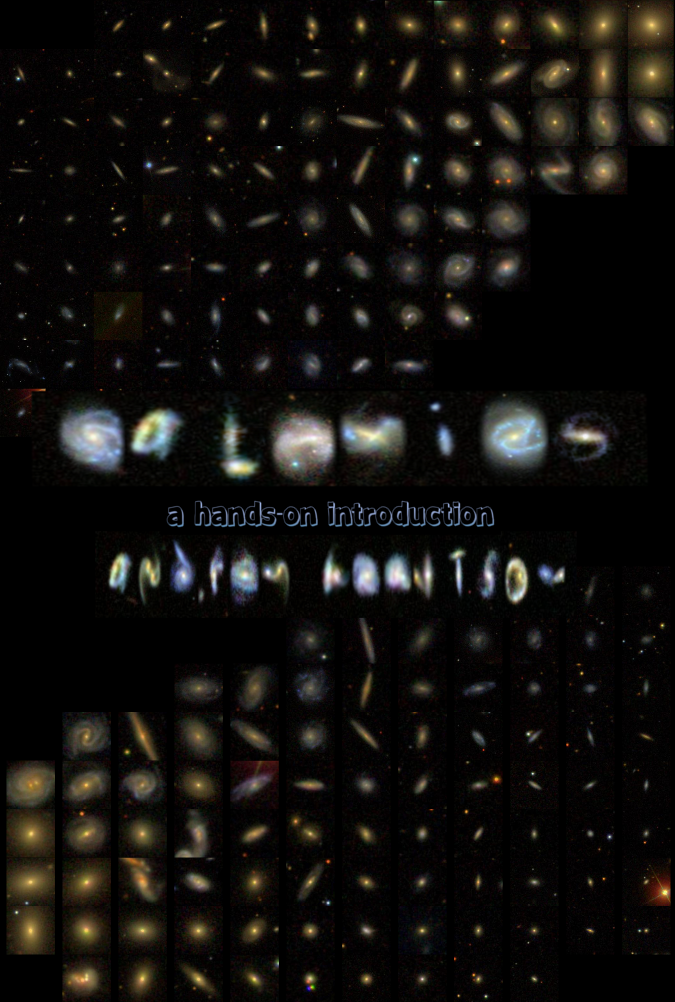
\includegraphics[width=\paperwidth]{cover}}; % Background image
%\draw[anchor=north] (midpoint) node [fill=ocre!30!white,fill opacity=0.6,text opacity=1,inner sep=1cm]{\centering\bfseries\sffamily\parbox[c][][t]{\paperwidth}{\centering\color{blue}{\fontsize{70}{80}\selectfont Galaxies}\\[15pt] % Book title
%{\Huge a hands-on introduction}\\[60pt] % Subtitle
%{\Huge Andrey Kravtsov}}}; % Author name
\end{tikzpicture}};
\end{tikzpicture}
\vfill
\endgroup

%----------------------------------------------------------------------------------------
%	COPYRIGHT PAGE
%----------------------------------------------------------------------------------------

\newpage
~\vfill
\thispagestyle{empty}

\noindent Copyright \copyright\ 2016 Andrey Kravtsov\\ % Copyright notice

\noindent \textsc{KICP Press}\\ % Publisher

\noindent \textsc{github.com}\\ % URL

\noindent Licensed under the Creative Commons Attribution-NonCommercial 3.0 Unported License (the ``License''). You may not use this file except in compliance with the License. You may obtain a copy of the License at \url{http://creativecommons.org/licenses/by-nc/3.0}. Unless required by applicable law or agreed to in writing, software distributed under the License is distributed on an \textsc{``as is'' basis, without warranties or conditions of any kind}, either express or implied. See the License for the specific language governing permissions and limitations under the License.\\ % License information

\noindent \textit{First printing, April 2016} % Printing/edition date

%----------------------------------------------------------------------------------------
%	Table of Contents
%----------------------------------------------------------------------------------------

%\usechapterimagefalse % If you don't want to include a chapter image, use this to toggle images off - it can be enabled later with \usechapterimagetrue

\chapterimage{uvhudf.PNG} % Table of contents heading image

\pagestyle{empty} % No headers

\tableofcontents % Print the table of contents itself

\cleardoublepage % Forces the first chapter to start on an odd page so it's on the right

\pagestyle{fancy} % Print headers again

%----------------------------------------------------------------------------------------
%	Chapters
%----------------------------------------------------------------------------------------


% if it ever gets so big as to require Parts
%\part{Part One}

\chapterimage{ch1_header.PNG} % Chapter heading image
%------------------------------------------------------------
\chapter{Galaxies: an overview of properties}
\label{ch:overview}
%------------------------------------------------------------
\begin{quote}
{\it “It is far more natural and conceivable to regard them as being not such enormous single stars but systems of many, whose distance presents them in such a narrow space that the light, which is individually imperceptible from each of them, reaches us on account of their immense multitude in a uniform pale glimmer. Their analogy with the stellar system in which we find ourselves, their shape, which is just what it ought to be according to our theory, the feebleness of their light which demands a presupposed infinite distance: all this is in perfect harmony with the view that these elliptical figures are just universes and, so to speak, Milky Ways, like those whose constitution we have just unfolded.”}  -- Immanuel Kant (1755)
\end{quote}

The term galaxy is derived from the Greek word ``galaxias'' ($\gamma\alpha\lambda\alpha\xi i\alpha\zeta$) which means ``milky'' and which was used to describe the milky band on the sky formed by stars within our Galaxy --- the Milky Way.\footnote{The connotation of the apparent Galaxy on the sky with milk is suprisingly universal and is present in most cultures. The two notable exceptions are the Ukrainian legend about a salt trader's way and the Cherokee legend about scattered cornbread crumbs. } Our Galaxy is only one out of two galaxies visible in the northern hemisphere and only one out of four visible to naked eye over the entire sky. 

Although many galaxies have been cataloged after the advent of observations with telescopes as ``nebulae,'' the name stemming from their nebulous appearance, their extragalactic nature was not understood until the 1920s. In fact, the name ``nebulae'' has persisted as the dominant names in astronomical literature through the mid-1930s. For example, the title of the seminal \href{http://adsabs.harvard.edu/abs/1929PNAS...15..168H}{\citet{hubble29}} paper presenting what we now call the Hubble law was  ``A Relation between Distance and Radial Velocity among Extra-Galactic Nebulae,'' which 
reflects the (then) new knowledge that galaxies are extra-galactic, but still uses the word ``nebulae.''\footnote{Hubble's 1934 book is still titled ``The realm of the nebulae'' \citep{hubble34}. The term ``galaxies'' only truly took off and displaced ``nebulae'' after 1940. See, e.g., \href{https://books.google.com/ngrams/graph?content=galaxies}{the use of word ``galaxies'' in books as a function of time} through Google's ngram-viewer.} 
% see e.g., https://books.google.com/ngrams/graph?content=galaxies%2C+galaxy&year_start=1800&year_end=2000&corpus=15&smoothing=3&share=&direct_url=t1%3B%2Cgalaxies%3B%2Cc0%3B.t1%3B%2Cgalaxy%3B%2Cc0


\section{Morphology}

\begin{quote}
{\it ``From a study of all available photographs with large reflectors, it is found that the characteristic features of non-galactic 
nebulae are rotational symmetry about dominating nuclei. 
About 2.5\% are irregular, lacking both these features, and form a homogeneous class of which the Magellanic Clouds are the 
most conspicuous members. The regular nebulae fall into a progressive sequence ranging from globular masses of unresolved nebulosity through lenticular forms to the open spirals 
with arms swarming with stars. This purely observational 
sequence conforms very closely to Jeans' theory of the origin 
and evolution of spirals.''} -- Edwin Hubble (1926, PASP)
\end{quote}

\begin{figure}[t]
\centerline{%
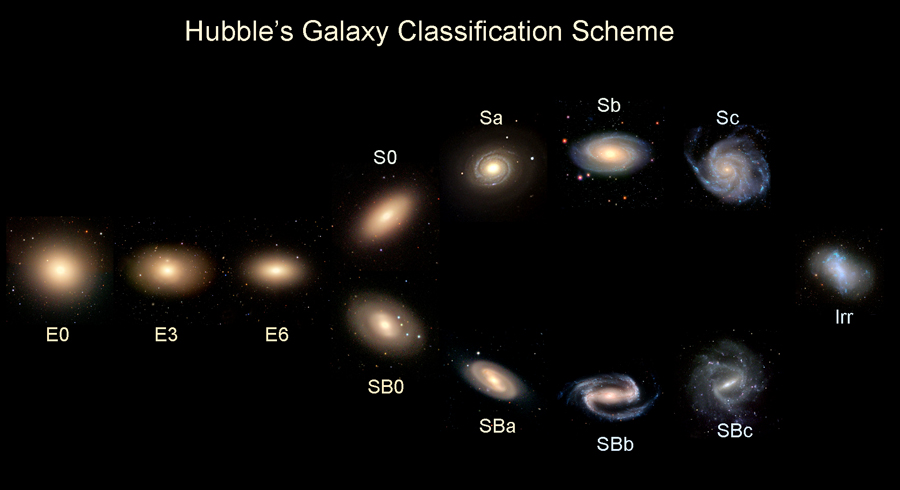
\includegraphics[scale=2.1]{fig/HubbleTuningFork.jpg}}
\caption{Hubble's famous tuning fork \protect\citep{hubble26}. This diagram was constructed by the \href{http://www.galaxyzoo.org/}{Galaxy Zoo} team using SDSS images. \label{fig:tuningfork}}
\end{figure}

Even before the extra-galactic nature of galaxies was proven beyond any doubt, people classified them based on their appearance or {\it morphology} using 
hand-sketches of how they appeared through a telescope.\footnote{For example, see sketches by William and \href{http://prints.royalsociety.org/artist/28272/john-frederick-william-herschel}{John Herschel}, \href{http://en.wikipedia.org/wiki/William_Parsons,_3rd_Earl_of_Rosse}{Lord Rosse} in the 19th century}. William Herschel introduced the notion of ``spiral nebulae'' in 1755 based on some of his sketches. In the same year, the German philospher Immanuel Kant, building upon earlier idea of Thomas Wright about the Milky Way as a disk of stars, put forth the idea that spiral nebulae were ``island universes'' of stars similar to our own Milky Way. 
The popularity of morphological studies and classification schemes is probably due both to the human tendency to classify as well as the relative success of the morphological classification approach in both the
biological sciences and in the classification of the photometric properties of stars. The popularity of Galaxy Zoo can attest that morphological classification comes naturally to the human brain, which evolved to see patterns even where there are none and suffers from curious idiosyncrasies \href{http://adsabs.harvard.edu/abs/2008MNRAS.388.1686L}{\citep{land_etal08}} when it comes to classifying patterns. 


The most persistent morphological classification scheme was developed by Hubble \href{http://adsabs.harvard.edu/abs/1926ApJ....64..321H}{\citep{hubble26}} and is usually represented via the ``tuning fork diagram'' (see Fig. \ref{fig:tuningfork}). Hubble developed this scheme  from the early 1920s to 1936 and it was definitely influenced by earlier ideas of Reynolds, who developed a classification based on the changing bulge-to-disk ratio of spirals.  Later, more elaborate schemes have also been developed  by de Vaucouleurs, van den Bergh, and others 
 \href{http://adsabs.harvard.edu/abs/2005ARA\%26A..43..581S}{\citep[see][for a comprehensive review]{sandage05}}, but these schemes are less widely used. 

Hubble's classification, in particular, was motivated by the evolutionary scenario advocated by James Jeans \href{http://adsabs.harvard.edu/abs/1919pcsd.book.....J}{\citep{jeans19b}}, in which spheroidal galaxies evolved into spirals by undergoing a sequence of transformations through intermediate morphologies. The bulge-less late-type spirals in this scheme were envisioned to be on the verge of break up into pieces that would then fly apart. The relative stages of this evolutionary sequence still reflected in the widely used terms ``early'' and ``late'' galaxies.

There is definitely value to classification  \href{http://adsabs.harvard.edu/abs/2005ARA\%26A..43..581S}{\citep[see, e.g.,][for discussion]{sandage05}} and sometimes classification does map onto key physical properties of the classified systems (e.g., the original spectral classification of stars mapped onto the sequence of effective temperatures of stars). When it comes to galaxies, none of the classification schemes have mapped onto any particular evolutinary scenario or physical processes, but they did provide a language for astronomers to talk about when they discuss galaxies. You should know this language because it will not go away any time soon. 

The minutae of morphological classication, such as the details of spiral structure, are probably not that important. First, they depend on the wavelength. Second, the morphology of galaxies becomes increasingly irregular and unclassifiable at higher redshifts (see Fig. \ref{fig:highz_morph}) and some of the morphological features are definitely transient features that can be triggered through tidal interactions (e.g., M51). Third, robust classification is difficult and requires sophisticated methods, such as neural networks, or human classifiers (the problem that was solved to some extent by the "citizen scientist" movement). 
This becomes increasingly difficult in the era of very large galaxy surveys. In the SDSS, for example, appearance of a galaxy becomes increasingly ``fuzzy'' beyond $\sim 200-300$ Mpc and details of morphology are difficult or impossible to discern. However, some key properties of these galaxies, such as color or concentration, can still be measured reliably. This is the reason why such quantities are increasingly used in lieu of morphology.

Nevertheless, the overall morphology of an individual galaxy and presence of structures, such as bulges, bars, or prominent spiral arms \emph{do} tell us useful information about the formation history or current dynamical state of the system. Thus, studies of galaxy morphology and how these features relate to systematic variations of galaxy properties continue unabated (e.g., \href{http://adsabs.harvard.edu/abs/2015ApJS..221....8H}{\citealt{huertas_company_etal15}}). The challenge, however, is that classification of large numbers of galaxies (by either human or automated computer algorithms) into fine morphological sub-classes is difficult for shallow surveys and/or distant galaxies. Thus, both automated and ``citizen science'' mass classifications use relatively coarse-grained, broad classes of elliptical, lenticular, and spiral classes (e.g., \href{http://adsabs.harvard.edu/abs/2011A%26A...525A.157H}{\citealt{huertas_company_etal11}}, \href{http://adsabs.harvard.edu/abs/2016arXiv160206854K}{\citealt{kuminski_shamir16}}).  
 
It makes sense then to also examine other ``broad brush'' properties of galaxies, such as luminosity, light profiles, surface brightness, concentration, colors, etc.  We will examine these properties and their mutual correlations as well as their correlations with morphology next. 

\begin{figure}[t]
\centerline{%
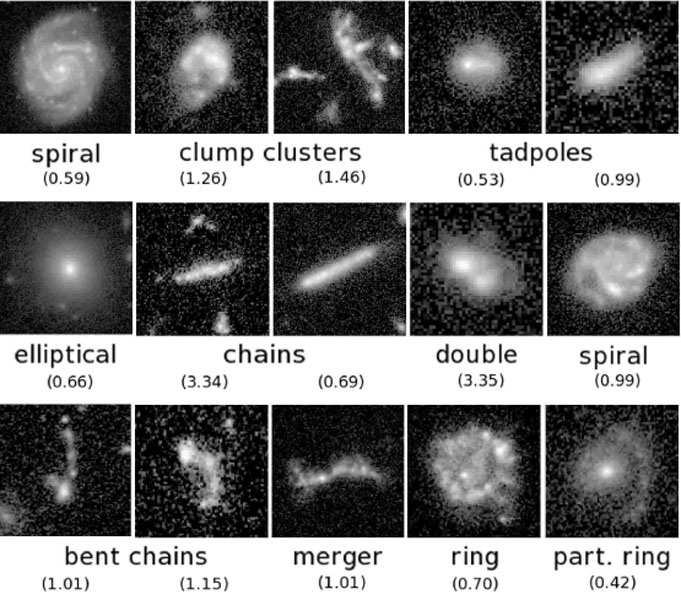
\includegraphics[scale=0.6]{fig/highz_morphology.jpg}}
\caption{Example of morphological classification at higher redshifts: $z$ is indicated in brackets under morphophological classification under each galaxy. At higher redshift we mostly observe light from shorter wavelength and galaxies are in earlier stages of their evolution. The fraction of "irregular" systems that do not fit into the main branches of the tuning fork grows steadily with increasing redshifts (although nice disks are found at least to $z\sim 3$). Here is an image with some new morphology "classes" at intermediate and higher $z$ from \protect\citep[][see \href{http://ned.ipac.caltech.edu/level5/Sept11/Buta/Buta_contents.html}{here} for the online version]{buta11}. \label{fig:highz_morph}}
\end{figure}

We will start with an overview and exploration of the basic galaxy properties using the Sloan Digital Sky Survey (SDSS) and other data sets. 
One way to get a feel for these properties is to try to construct your own version of the Hubble's tuning fork diagram by finding random examples of galaxies of each morphological 
class and examining their key properties: spectra, color, luminosity, size, and bulge-to-disk ratio, as well as useful quantities derived from these, such as surface brightness. 
For example, even a quick examination of the tuning fork diagram in  
 Figure \ref{fig:tuningfork} shows that the sequence does correspond to 
a regular trend in color of galaxies. The trend in color means a trend in spectral shapes, which, in turn, implies a trend in properties of stellar populations (age, metallicity, dust, etc.). 

\section{Galaxy magnitudes and luminosities}

Astronomers use a logarithmic magnitude scale to quantify the apparent and intrinsic brightness of sources, which is akin to the historical visual magnitude system based on the roughly logarithmic sensitivity of our eyes.\footnote{The actual sensitivity of the human eye is complicated and is currently a subject of continued study. It may be closer to a square root response than to a logarithmic response.}
A number of different magnitude systems exist in the literature, especially in older papers. Modern magnitude systems, e.g. in SDSS, are based on the AB-magnitude system \href{http://adsabs.harvard.edu/abs/1983ApJ...266..713O}{\citep{oke_gunn83}}, which is described in detail in \href{http://adsabs.harvard.edu/abs/1996AJ....111.1748F}{\citet{fukugita_etal96}}.\footnote{See also online info  \href{http://classic.sdss.org/dr3/algorithms/fluxcal.html}{here}.}

In practice magnitudes are defined using light from a limited range of wavelengths, defined by a filter. In the AB system this is given by \href{http://adsabs.harvard.edu/abs/1996AJ....111.1748F}{\citep[][]{fukugita_etal96}}:
\begin{equation}
m_f =-2.5\log_{10}\frac{\int f_{\nu}S(\nu) d(\log_{10}\nu)}{\int S({\nu}) d(\log_{10}\nu)} - 48.6,
\label{eq:magforcolorAB}
\end{equation}
where $f_\nu$ is the specific flux per unit frequency.

The SDSS filter transmission curves, $S_\lambda$, can be found \href{http://classic.sdss.org/dr7/instruments/imager/filters/}{\underline{here}}.  SDSS database reports spectra as the flux density per unit wavelength at a given $\lambda$, $f_\lambda$,  instead of $f_\nu$.  Converting from $f_\nu$ to $f_\lambda$  ($\nu=c/\lambda$, $d\nu=-cd\lambda/\lambda^2$, so $f_\nu=\lambda^2 f_\lambda/c$), the magnitude in a given 
filter can be expressed as  \href{http://adsabs.harvard.edu/abs/2006MNRAS.371..121S}{\citep[see, e.g., eqs 2 and 3 in][]{smolcic_etal06}}:
\begin{equation}
m_f =-2.5\log_{10}\left[\frac{10^{19.44}}{c}\frac{\int f_{\lambda}S(\lambda)\lambda d\lambda}{\int S({\lambda})\lambda^{-1} d\lambda}\right].
\label{eq:magforcolor}
\end{equation}

The flux density, $f_\lambda$, has a simple meaning, but its measurement is often non-trivial in practice because it requires integration of photons over some area on the sky. For point sources like stars and quasars the total flux can simply be collected from an area that encloses the telescope point spread function, although for stars in crowded regions even this task is non-trivial. Galaxies, however, are intrinsically extended and diffuse (as discussed earlier, this is the reason they were dubbed ``nebulae'') and collecting flux associated with galaxies requires either defining a galaxy boundary or devising some way to calculate the total flux. 

As we will see below, different ways of doing this may result in significantly different estimates of galaxy intrinsic luminosities. Thus, although this subject may seem technical it is actually quite important to understand how total flux is estimated for galaxies. To understand how this is done or how it should be
done, we need to discuss the radial distribution of light around galaxies. 

\section{Surface brightness profiles}

Galaxy surface brightness is defined as the amount of light that we receive from a given area of the galaxy. This quantity makes sense for extended objects where we can compare amount of light we get from an area from the total amount of light we can get from a point source (see, e.g., S 5.1.2 in the SG book). 
Even if we don't know the distance to a galaxy we can compute the surface brightness in units of magnitude per square arcsec - i.e., the flux in the $r$-band magnitudes we receive from a solid angle $d\Omega$ in $\mathrm{arcsec}^2$: \footnote{Why is it meaningful to compute and consider surface brightness in such units?}

\begin{equation}
\mu_{\rm f}=-2.5\log_{10}(f_{\rm f}/d\Omega) + \mathrm{const}=m_{\rm f}+2.5\log_{10}d\Omega, 
\label{eq:mur}
\end{equation}
where $f_{\rm f}$ is the flux collected from the solid angle on the sky $d\Omega$ (usually, in square arcseconds). 
The choice of  $d\Omega$ depends on one's goals. For example, we can define $d\Omega$ to be an annulus of radius $R$ and thickness $\Delta R$, as is done in the estimates of the Petrosian magnitudes. 
Or we can estimate surface brightness in equal size patches of a given $d\Omega$.

Note that we can always express the flux $f_{\rm f}$ in equation \ref{eq:mur} in terms of intrinsic luminosity in the same filter: $f_{\rm f}\propto L_{\rm f}/d^2$, where $d$ is galaxy distance. Thus, $\mu_{\rm f}$ and  $\Sigma_{\rm f}=L_{\rm f}/\mathcal{A}$, where $\mathcal{A}$ is a physical area (e.g., in $\mathrm{kpc}^2$), are tightly related (see eq. \ref{eq:musb} in \S \ref{sec:surface_brightness} for the exact relation) and we can talk about $\mu_{\rm f}$ and $\Sigma_{\rm f}$ interchangeably.  Often, $L_{\rm f}$ is also converted into an estimate of stellar mass of the underlying stellar population stellar using some type of population modelling, as discussed below. In these cases we talk about stellar surface density, $\Sigma_\ast$. 

\begin{figure}[t]
\centerline{
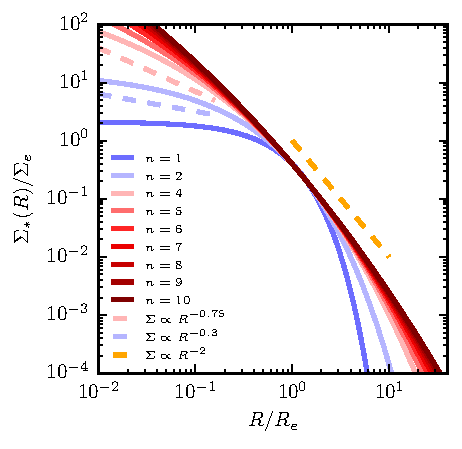
\includegraphics[scale=1.75]{fig/sersic_pro.pdf}
}
\caption{The S\'ersic surface density profiles for $n\in[1,10]$ along with three power laws for illustration.  \label{fig:sersic_pro}}
\end{figure}


\subsection{Exponential, de Vaucouleurs, and S\'ersic profiles}

The measured surface brighness profiles of galaxies are often parameterized using simple functional forms. 
The most frequently used forms are the exponential profile which tends to provide a better fit to the surface brightnesses of disky galaxies and the de Vaucouleurs profile \href{http://adsabs.harvard.edu/abs/1953MNRAS.113..134D}{\citep{devaucouleurs53}} that tends to provide a better fit to profiles of  spheroidal systems.\footnote{\href{http://adsabs.harvard.edu/abs/1930ApJ....71..231H}{\citet{hubble30}} proposed another form to describe profiles of spheroidal galaxies, given by $\mu\propto 5\log(1+R/R_e)$. This form does fit many {\it bright} spheroidal galaxies quite well, but is too shallow in the central regions for many other early type systems (see Figure \ref{fig:sersic_pro}).} 

The exponential and de Vaucouleurs profiles are specific cases of a more general \citet{sersic68}  profile:

\begin{equation}
\Sigma(R)=\Sigma_e\exp\left\{-b_n\left[\left(\frac{R}{R_e}\right)^{1/n}-1\right]\right\},
\label{eq:serspro}
\end{equation}
where $\Sigma_e$ is the surface brightness at the effective radius $R_e$ that encloses half of the total light from the model. The constant $b_n$ is related to $n$ -- the S\'ersic index -- that controls the overall shape of the profile.  Its detailed properties are well described by \href{http://adsabs.harvard.edu/abs/2005PASA...22..118G}{\citet{graham_driver05}}.\footnote{See \href{http://ned.ipac.caltech.edu/level5/March05/Graham/Graham2.html}{here} for version online.} In particular, $b_n = 1.9992n - 0.3271$. This is an approximation, but a very accurate one. The profile above is sometimes expressed as
\begin{equation}
\Sigma(R)=\Sigma_0\exp\left[-\left(\frac{R}{R_d}\right)^{1/n}\right],
\label{eq:serspro2}
\end{equation}
where $\Sigma_0=\Sigma_e \exp(b_n)$ and $R_d\equiv R_e/b_n^n$ is the scale length. 

If profiles are constructed using magnitudes rather than surface brightness or intensity, the corresponding expression is:  
\begin{equation}
\mu(R)=\mu_e+\frac{2.5b_n}{\ln(10)}\left[\left(\frac{R}{R_e}\right)^{1/n}-1\right], 
\label{eq:serpro}
\end{equation}
where $R_e$ is the half-light radius and $n$ is the S\'ersic index. 

The exponential profile is given by $n=1$ case:
\begin{equation}
\mu(R)=\mu_e+\frac{2.5b_1}{\ln(10)}\left[\frac{R}{R_e}-1\right],
\label{eq:exppro}
\end{equation}
where $b_1=1.678$. $R_e$ defined here encloses half of the total light of the profile. Note that this linear increase in magnitude per area corresponds to an exponential decrease in luminosity per area, thus the name. The de Vaucouleurs profile is given by $n=4$:
\begin{equation}
\mu(R)=\mu_e+\frac{2.5b_4}{\ln(10)}\left[\left(\frac{R}{R_e}\right)^{1/4}-1\right],
\label{eq:devpro}
\end{equation}
where $b_4=7.669$. Here too $R_e$ encloses half of the light is enclosed within $R_e$.
Note that in the figures below, surface brightness is plotted in terms of surface mass density; these are related to $\mu$ via eq. \ref{eq:musb} in \S \ref{sec:surface_brightness}.

Although pure exponential and de Vaucouleurs profiles \emph{do} provide a good description of the surface brightness profiles of some galaxies, examination of large samples shows that they are over simplifications of the typical profiles (see Figure \ref{fig:gal_spro} below). 

The approximate 3D deprojected profile of the projected S\'ersic profile is discussed in \href{http://adsabs.harvard.edu/abs/1999MNRAS.309..481L}{\citet{lima_neto99}}. A good approximation for the 3D profile that gives the S\'ersic profile in projection is given by the \citet[][]{einasto65} profile that is the second most commonly used profile to describe the radial density profiles of dark matter halos in simulations of structure formation \citep[see][for detailed information about this profile]{merritt_etal06} . 
Analytical functions of the 3D profiles corresponding to exponential and de Vaucouleurs profiles are also discussed by \href{http://adsabs.harvard.edu/abs/1997MNRAS.288..457P}{\citet{pitts_tayler97}} and \href{http://adsabs.harvard.edu/abs/1990ApJ...356..359H}{\citet{hernquist90}}, respectively. Note though that this deprojection of the exponential profile makes sense for a spherical distribution, not for disk distribution of stars. 

Figure~\ref{fig:sersic_pro} shows S\'ersic profiles for $n\in[1,10]$. 
Note the main difference between $n=1$ and $n=4$ profiles is in the central regions, where the exponential profile is shallow, while the de Vaucouleurs profile is steep. At the largest radii the exponential profile becomes steeper due to the higher power of $R/R_e$ in the exponent. As we will see below, profiles of most galaxies are not traced to sufficiently large radii for this difference to be apparent. Note, also, that there is a fairly wide range of intermediate radii (nearly a decade), where the exponential and de Vaucouleurs profiles are close to each other. For $n>6$, the profile shape changes only mildly with increasing $n$. This property sometimes leads to fit degeneracies, where best fit values of $n$ are driven to large values. At large $R$, the profiles are close to $\Sigma\propto R^{-2}$ independent of $n$. This asymptotic behavior can be understood analytically in the limit of large $R$ and $n$ - see the last paragraph in S 2.1 of \href{http://ned.ipac.caltech.edu/level5/March05/Graham/Graham2.html}{\citet{graham_driver05}}. 

\subsection{Surface brightness profiles of spheroidal galaxies}

The left panel of Figure \ref{fig:gal_spro} shows  the S\'ersic profiles of a couple hundred nearby ($z<0.1$) spheroidal galaxies with stellar masses in the range
$\log_{10}(M_*/M_\odot)\in [10.7, 11.6]$ from \href{http://adsabs.harvard.edu/abs/2013ApJ...763...73S}{\citet{szomoru_etal13}}.
The profiles are colored by the stellar mass of the galaxies with darker red colors representing more massive, i.e. more luminous, galaxies. 

The solid orange line shows the de Vaucouleurs profile. It is definitely a good description for some of the galaxies, but it is clear that profiles of spheroidal galaxies have a range of $n$ values. 

Also, the dashed orange line shows the profile \href{http://adsabs.harvard.edu/abs/1930ApJ....71..231H}{\citet{hubble30}} proposed for elliptical galaxies. As you can see, it is not a bad description of the modern measurements, although individual galaxies do exhibit a diversity of profile shapes. Note that some galaxies have rather cored profiles, as implied by the Hubble's form, while others have cuspy profile (surface density continuing to increase towards smaller radii). There are arguments that there is a real dichotomy in the profiles of spheroidal galaxies \href{http://adsabs.harvard.edu/abs/1997AJ....114.1771F}{\citep[e.g.,][]{faber_etal97}}. 
Brightest galaxies tend to have cored profiles. Not surprisingly, Hubble made his measurements for the brightest spheroidals and this is probably why he came up with the profile that is quite flat in the center. 

\begin{figure}[ht]
\centerline{
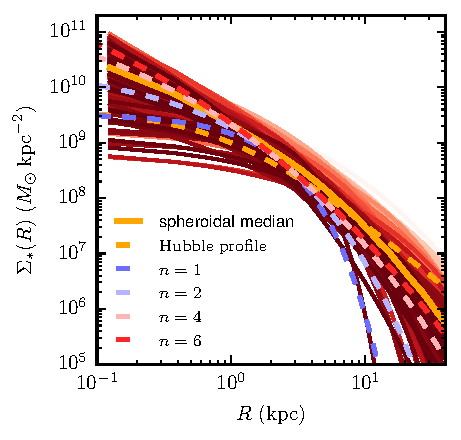
\includegraphics[scale=1.05]{fig/szomoru_pro.pdf}
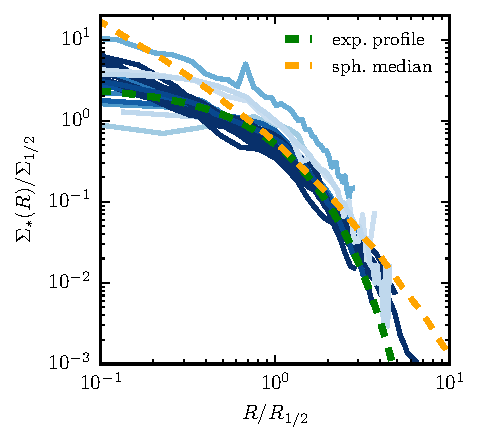
\includegraphics[scale=1.05]{fig/things_pro.pdf}
}
\caption{Left  panel:  the S\'ersic profiles of a couple hundred nearby ($z<0.1$) spheroidal galaxies with stellar masses in the range
$\log_{10}(M_*/M_\odot)\in [10.7, 11.6]$ from \href{http://adsabs.harvard.edu/abs/2013ApJ...763...73S}{\citet{szomoru_etal13}}.
The profiles are colored by the stellar mass of the galaxies with darker red colors representing more massive, i.e. more luminous, galaxies. Right panel: surface density profiles of the THINGS galaxies spanning 
a wide range of stellar masses $\log_{10}(M_*/M_\odot)\in [7, 11]$. The green curve shows the exponential profile with normalization corresponding to the parameters of the Milky Way. To take away wide variation of galaxy sizes, the radii are normalized by the half-mass radius of each galaxy, while surface densities are normalized by $\Sigma_{1/2}=M_*/(2\pi R_{1/2}^2)$.  The profiles are colored with logarithm of stellar mass with lighter blue corresponding to lower stellar masses. The figure shows that $\Sigma_*/\Sigma_{1/2}$ is larger for dwarf galaxies in these rescaled units, which reflects their systematically lower surface densities $\Sigma_{1/2}$. The dashed orange line is the normalized median profile of spheroidal galaxies.   \label{fig:gal_spro}}
\end{figure}

\subsection{Surface brightness profiles of late type disk galaxies}

The right panel of Figure \ref{fig:gal_spro} shows the stellar surface density profiles of late-type disk galaxies in the combined THINGS and LITTLE THINGS sample which spans
a wide range of stellar masses $\log_{10}(M_*/M_\odot)\in [7, 11]$. The green curve shows an exponential profile with normalization corresponding to the parameters of the Milky Way. To take away wide variation of galaxy sizes, the radii are normalized by the half-mass radius of each galaxy, while surface densities are normalized by $\Sigma_{1/2}=M_*/(2\pi R_{1/2}^2)$.  The profiles are colored by the logarithm of stellar mass with lighter blue corresponding to lower stellar masses. The figure shows that $\Sigma_*/\Sigma_{1/2}$ is larger for dwarf galaxies in these rescaled units, which reflects their systematically lower surface densities $\Sigma_{1/2}$.

The figure shows that the exponential profile is a reasonable description of the surface density profiles. Nevertheless, many profiles are somewhat shallower than exponential in the outer regions and steeper than exponential in the center. The latter is often due to the presence of central mass concentration in the form of a bar or a bulge. Such concentration are not well fit by the exponential profile, which motivates fits of profiles with varying S\'ersic index $n$ or multi-component fits to $\Sigma(R)$. 

Figure \ref{fig:gal_spro} also show the median surface density profile of spheroidal galaxies. The radii in this case are normalized to the median half-mass radius, while vertical normalization is $\xi \bar{M}_*/(2\pi \bar{R}_{1/2}^2)$, where $\bar{M}_*$ and $\bar{R}_{1/2}$ are the median stellar and half-mass radii and $\xi$ is a factor adjusted so that the normalized profile roughly matches that of the exponential profile at $R\approx R_{1/2}$. Figure shows that the median profile of spheroidal galaxies is actually quite close to the profiles of late type galaxies at $R\gtrsim R_{1/2}$, and the main difference is at smaller radii: the central surface densities of spheroidal galaxies are larger than those of spiral galaxies (see \href{http://adsabs.harvard.edu/abs/2013ApJ...764L..31K}{\citealt{kravtsov13}} for additional discussion on this). One implication of this fact is that one cannot turn a spiral galaxy into spheroidal by simply stopping star formation and letting stellar distribution fade and become red. Redistribution of stellar mass must occur in the process (\href{http://adsabs.harvard.edu/abs/2013ApJ...776...63F}{\citealt{fang_etal13}}).

\subsection{Multi-component descriptions of the surface brightness profiles}
\label{sec:spro_multicomp}

Galaxies with both a spheroidal component (e.g., bulges and bars) and a disk component are commonly modelled as a sum of the exponential disk and de Vaucouleurs bulge. 
In the main SDSS sample we've been examining, the {\tt fracdeV} parameter is an indicator what fraction of light is well fit by the de Vaucouleurs profile. This is a rough indication of the fraction of light in spheroidal component.  Nowadays, surface density profiles of late type disk galaxies are often fit with  two S\'ersic components with independent $n$ values. 

Purely spheroidal galaxies were thought to be much simpler and well-described by a single S\'ersic component. However,  a number of recent studies have shown that if one analyzes surface density profiles of ellipticals in detail, they actually require 2 or 3 Sersic components to fit accurately. This was first found for the Brightest Cluster Galaxies (BCGs), in which the inner light distribution is described by the usual high-$n$ de Vaucouleurs like profile, but the outer component is often described by a much flatter profile with $n\sim 1$ (\href{http://adsabs.harvard.edu/abs/2007MNRAS.378.1575S}{\citealt{seigar_etal07}}, \href{http://adsabs.harvard.edu/abs/2014arXiv1401.7329K}{\citealt{kravtsov_etal14}}). \href{http://adsabs.harvard.edu/abs/2013ApJ...766...47H}{\citet{huang_etal13a}} showed that two or three S\'ersic components are required to accurately describe surface brightness profiles of all elliptical galaxies, with the outer components tending to have low values of $n$. 
In the single S\'ersic component fits to such galaxies $n$ is driven to large values \href{http://adsabs.harvard.edu/abs/1996ApJ...465..534G}{\citep{graham_etal96}}.

The reason multiple components have not been detected earlier is because they are relatively subtle and require accurate measurements of profile at low surface brightnesses (which is difficult due to sky background). The existence of these distinct components indicates different formation mechanisms likely corresponding to different stages of evolution of early-type galaxies (inner regions are built up during early stages, while the outer profiles are built during late stages by accretion of other galaxies rather than by {\it in situ} star formation). 

The outer regions of disks exhibit variation from a sharp cutoff to a more steady decline (e.g., \href{http://adsabs.harvard.edu/abs/2006A%26A...454..759P}{\citealt{pohlen_trujillo06}} and \S 3.8 of \href{http://adsabs.harvard.edu/abs/2009ARA%26A..47..159B}{\citealt{blanton_moustakas09}}).  

%-------------------------------------------------------------
\section{Galaxy magnitudes and luminosities}
%------------------------------------------------------------

Now that we are familiar with the surface brightness profiles of galaxies, we can discuss various methods for estimating galaxy magnitudes (and thus luminosities, if the distance to the galaxy is known). 

One thing that is clear from Figure \ref{fig:gal_spro} and the discussion in \S \ref{sec:spro_multicomp} is that the light distribution in galaxies extends to large radii. In fact, our ability to trace it is typically limited by the sensitivity of observations. This would not be an issue if the fraction of light at large radii was small. This is indeed the case for steeply falling profiles, such as the exponential profile. However, Figure \ref{fig:gal_spro} shows that the profiles of many spheroidal galaxies have outer slopes comparable to that predicted by the Hubble profile: $\Sigma\propto R^{-2}$, for which the total luminosity diverges logarithmically: $L(<R)\propto \int_0^R\Sigma(R)RdR\propto \ln R$. Thus, in galaxies with such profiles a large fraction of the total light may be contributed by the low surface brightness outer regions that may actually be below the sensitivity of observations, defined by the observation-specific level of background. 

In practice, this is addressed in two ways. First, one can simply define the total magnitude as an {\it aperture magnitude} within a certain well-defined radius, ignoring light beyond it. Second, one could try to construct the best possible model for the distribution of light using the portion of the galaxy that is reliably measured in observations and compute the total light by extrapolating the model profile. In the SDSS  magnitudes obtained in this way are called {\it model magnitudes}.

Once the apparent magnitude for a galaxy is estimated using one of these approaches, the absolute magnitude and luminosity can be computed if the galaxy distance or redshift are known using the equations \ref{eq:mM} and \ref{eq:LMf} in  \S \ref{sec:mML}.
 
\subsection{Aperture, Holmberg, and Petrosian magnitudes}
\label{sec:apermags}

One of magnitudes provided in the SDSS database, called $m_{\rm fiber}$, is based on light integrated within a fixed aperture of radius $1.5^{\prime\prime}$. However, it is a bad idea to use such fixed aperture magnitudes for physical studies of galaxies, because this would correspond to different physical scales for galaxies of different intrinsic size and galaxies of the same type but at different distances. 

An example of a radius definition that does not suffer from these problems is the {\it Holmberg radius\/}, defined as the major axis of the observed galaxy's ellipsoidal light distribution. which itself is defined as the contour at which surface brightness of a galaxy in the $B$ band is equal to $26.5$  magnitudes per square arcsecond \href{http://adsabs.harvard.edu/abs/1958MeLuS.136....1H}{\citep{holmberg58}}. Similar definitions could of course be used for other bands. This definition works as long as observations allow for measures of surface brightness to $26.5\rm\ mag\,arcsec^{-2}$ reliably. What if this is not the case, like when a galaxy is far away or when observations are shallow?

\href{http://adsabs.harvard.edu/abs/1976ApJ...209L...1P}{\citet{petrosian76}} proposed to measure radii based on the integrated galaxy flux to make such estimates more robust. The idea is that as one traces the surface brightness profile $\Sigma(R)$, one can compare the light within some shell of thickness $\Delta R/R$, $\Delta I$, to the total light within $R$, $I(<R)$ and define the galaxy radius as the radius corresponding to $\Delta I=\eta I(<R)$. One could then tune $\eta$ in such a way that the measurement recovers all or most of the flux for a particular assumed form of the profile $\Sigma(R)$ extending to infinity. The specific implementation of the Petrosian magnitude and sizes in the SDSS pipeline is desribed in \S \ref{sec:petromagsize}.

 One can show that theoretically the Petrosian magnitudes defined as in the SDSS should recover almost all of the flux of an exponential galaxy profile and about 80\% of the flux for a de Vaucouleurs profile.
 As we discussed above, however, galaxy surface brightness profiles are often described by different functions (corresponding to different components) at different radii. Thus, in practice the Petrosian magnitude may underestimate total galaxy light by $\approx 0.2-0.5$ mag. The magnitude of the underestimate depends on the fraction of light in the outer component, which increases with increasing galaxy luminosity. 
 
 Thus, this underestimate will affect the brightest galaxies the most \href{http://adsabs.harvard.edu/abs/2013MNRAS.436..697B}{\citep[see][]{bernardi_etal13}}. This issue will come up in the practical calculation of the galaxy luminosity function we will discuss below. 

\subsection{Model magnitudes}

An alternative way is to estimate total magnitude by using an extrapolation of the model for surface brightness profiles obtained via a fit to the regions of the galaxy where the light profile is measured reliably. One could, for example, perform a fit of one of the surface brightness profile models discussed above or their combination \citep[e.g., see][for a recent example of such fits for SDSS galaxies]{meert_etal15}. The total model magnitude is then obtained by integrating the best fit model profile to infinity. 

The SDSS pipeline measures \href{http://classic.sdss.org/dr7/algorithms/photometry.html}{two kinds of model magnitudes} based on fits of the exponential and de Vaucouleurs profiles to each galaxy in the $r$-band (the most sensitive band). The goodness of fit is evaluated for each of these models and the profile 
providing a better fit is chosen as the surface brightness profile model for computing SDSS model magnitudes. The model magnitudes are then computed by integrating this model to infinity.

On the other hand, {\it cmodel magnitudes}\/ use  surface brightness profile model constructed as a linear combination of  the exponential and de Vaucouleurs models used to define model magnitudes in the $r$ band: $F_{\rm composite} = {\rm fracDeV} \cdot F_{\rm deV} + (1 - {\rm fracDeV}) F_{\rm exp}$,
where $F_{\rm deV}$ and $F_{\rm exp}$ are the de Vaucouleurs and exponential surface brightness profiles computed using the corresponding independent model fits in the $r$ band. The cmodel magnitude is computed using fracdeV value that fits they surface brightness profile of a particular galaxy best. These magnitudes are recommended as the best choice for estimating galaxy luminosities and other physical properties. As we will see below, however, for bright galaxies they underestimate the total light.

We will also use magnitudes obtained for SDSS galaxies using the S\'ersic profiles or multi-component fits by \citet{meert_etal15}. 
In general, such magnitudes will give a result different from that given by the Petrosian magnitude definition or by the model and cmodel magnitude algorithms described above. For example, \href{http://adsabs.harvard.edu/abs/2005AJ....130.1535G}{\citet{graham_etal05}} provide fitting formulae for correcting the Petrosian magnitudes to account for the total light in the Sersic profile of a given $n$. 

%---------------------------------------------------------
\section{Luminosity distribution of galaxies}
%---------------------------------------------------------

%\begin{figure}
%\centerline{
%\includegraphics[scale=1.5]{fig/mz_sdss.pdf}}
%\caption{Distribution of galaxies of the SDSS main sample in the redshift -- $r$-band magnitude plane. The red dashed line shows the relation for galaxies of fixed absolute magnitude of $M_r=-22$. \label{fig:mzsdss}}
%\end{figure}

\begin{figure}
\centerline{
\includegraphics[scale=1.1]{fig/mappz_sdss.pdf}
\includegraphics[scale=1.1]{fig/Mabsz_sdss.pdf}}
\caption{Left panel: apparent Petrosian $r$-band magnitude versus redshift $z$. The red dashed line shows expected $m(z)$ for an object of constant $r$-band absolute magnitude of $M_r=-23$. The orange and yellow lines correspond to an object of $M_r=-23$ at $z=0$, but which is assumed to get brighter with redshift as $1.3z$ (orange) and which is $k$-corrected (yellow). Right panel: distribution of galaxies from the SDSS main sample in the redshift -- $r$-band Petrosian absolute magnitude plane. The magenta dashed line shows the absolute luminosity limit corresponding to the apparent magnitude limit of $m_{\rm lim, r}=17.7$ for the main SDSS spectroscopic galaxy sample.  The other lines are the same as in the left panel. \label{fig:Mzsdss}}
\end{figure}

Figure \ref{fig:Mzsdss} shows the distribution of galaxies in the SDSS main galaxy sample in the plane of redshift and absolute $r$-band Petrosian magnitude. Galaxies at a given $z$ are approximately at the same distance from us\footnote{Can you explain why this is only approximately true?} and thus the distribution of galaxies in a vertical band of a given $dz$ shows us the distribution of galaxies as a function of their intrinsic luminosity in that redshift interval --- or {\it the galaxy luminosity function}. We can see that galaxies have a wide range of intrinsic luminosities.

This may seem trivial to you, but it took more than two decades for people in 1920s-1940s to realize this basic fact. When Hubble was considering galaxies in the samples he used for his work on expansion of the universe, he found that fainter galaxies had to have larger distances and he has postulated that galaxies have a narrow range of intrinsic luminosities with a Gaussian distribution. If you take a look at his seminal paper on the cosmic expansion, you will see that Hubble actually used apparent magnitudes to estimate distances to some of the galaxies -- i.e., he treated galaxies as standard candles. 

It was only around 1943 that Fritz Zwicky realized that the universe is full of intrinsically faint galaxies from his studies of the Local Group neighborhood and distant galaxy clusters (where galaxies can be assumed to be at roughly the same distance). Zwicky then argued that galaxies had a broad range of intrinsic luminosities and that their luminosity distribution at low $L$ was flat. We can see that this basic assessment is correct for the distribution of galaxies in $M_r$ at a given $z$ in Figure \ref{fig:Mzsdss}.

The upper envelope shown in Figure \ref{fig:Mzsdss} by the dashed red line simply corresponds to the apparent magnitude limit of the main SDSS spectroscopic galaxy sample of $m_{\rm lim, r}=17.7$:
$M_{r}= m_{r,\rm lim}+5\log_{10}\left(d_{\rm L}/10\,\mathrm{pc}\right)$. The actual completeness is 0.93 near the limit and is then slowly decreasing with decreasing apparent magnitude (see e.g., Fig. 2 in \href{http://adsabs.harvard.edu/abs/2009MNRAS.399.1106M}{\citealt{montero_dorta_prada09}}).

The figure shows that fainter galaxies (larger $M_r$) dominate by number and that there is a rather sharp cutoff in the number of galaxies with luminosities larger than a given threshold of $M_{r}\approx -22$. This sharp threshold changes somewhat to brighter values with increasing $z$. This increase is due to two factors: 1) the volume covered by the SDSS is increasing with increasing $z$, so brightest rarest galaxies are becoming more common and 2) luminosities of galaxies actually evolve across this redshift interval so that galaxies at larger $z$ are intrinsically brighter. Thus, we can deduce the overall shape of the distribution of galaxy luminosity and rough sense of evolution right away from this plot. 

\begin{figure}
\centerline{
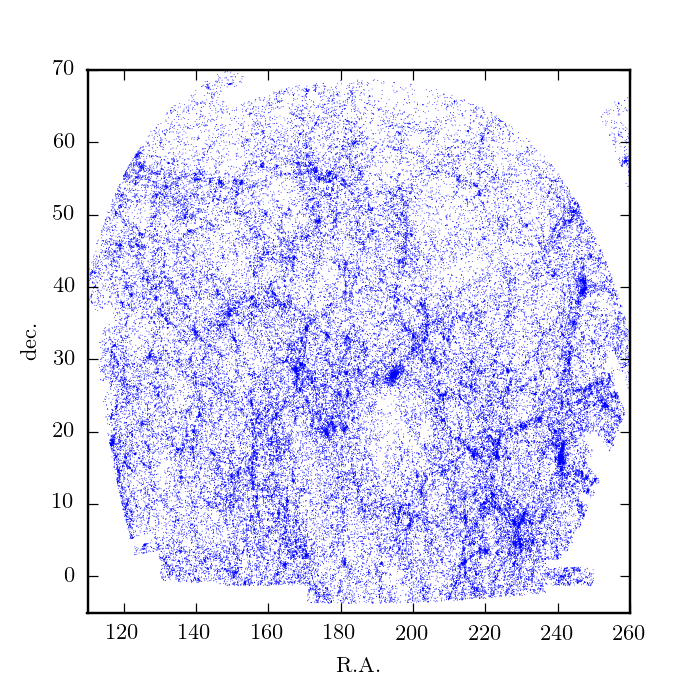
\includegraphics[scale=0.85]{fig/sky_lss_z006.png}
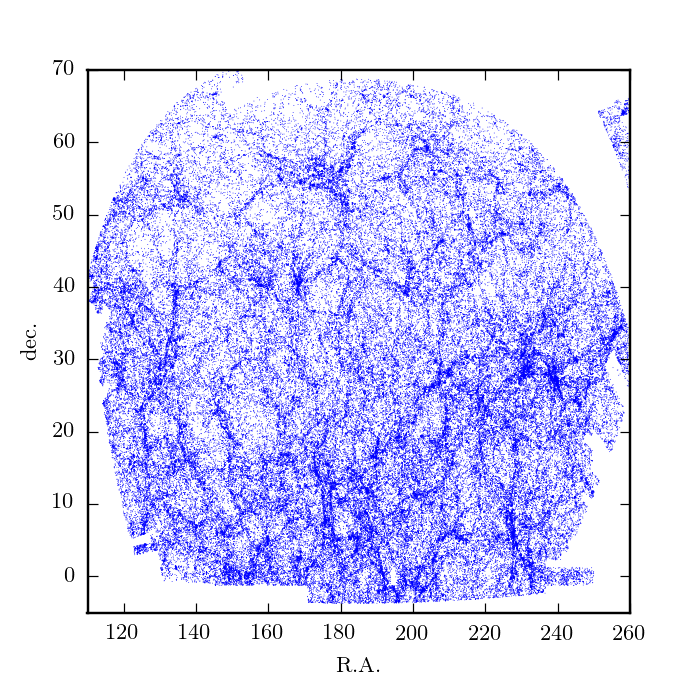
\includegraphics[scale=0.85]{fig/sky_lss_z010.png}}
\caption{Left panel: distribution of the SDSS galaxies with $z<0.06$ in the main northern region of the survey. Right panel: the same but for galaxies in the redshift interval $0.06<z<0.1$.
The bottom of the region in this $z$ interval contains many more prominent structures, including the SDSS Great Wall \protect\href{http://adsabs.harvard.edu/abs/2005ApJ...624..463G}{\citep{gott_etal05}}. \label{fig:sky_lss}}
\end{figure}

The figure also shows prominent vertical stripes in distribution of galaxies in $z$ direction. These stripes reflect large-scale structure in the galaxy distribution, which we will discuss in more detail below. In particular, 
the sharp feature at $z\approx 0.02$ is due to the supercluster associated with the Coma cluster of galaxies. 
The prominent wide stripe at $z\approx 0.07$ is due to the largest structure in the distribution of galaxies that was identified so far --- the SDSS Great Wall \href{http://adsabs.harvard.edu/abs/2005ApJ...624..463G}{\citep{gott_etal05}}. This structure is within the bottom of the region shown in the right panel of Figure \ref{fig:sky_lss} along with other prominent structures.
The figure shows the cosmic web like distribution of galaxies in both redshift intervals shown in two panels. However, it is clear that the redshift interval $0.06<z<0.10$ contains much more prominent large-scale structures at the bottom of the region.

Large-scale structure as traced by galaxies of different properties is interesting in its own right and we will return to it later. For the purposes of studying the number density of galaxies, however, it causes variations. For example, it is clear from Figures \ref{fig:Mzsdss} and \ref{fig:sky_lss} that if we estimated the number density of galaxies as a function of luminosity in the redshift range of $0.03<z<0.05$, we would get a considerably lower value than if we did this in $0.07<z<0.09$. Such variations are called {\it sample variance} (e.g., \href{http://adsabs.harvard.edu/abs/2003ApJ...584..702H}{\citealt{hu_kravtsov03}}) and are one of the sources of uncertainty in the estimation of galaxy abundance as a function of intrinsic luminosity --- the luminosity function. So much so that the SDSS Great Wall region is often excluded when various galaxy statistics are computed. 
 The other source is the usual Poisson noise due to there being a finite number of galaxies. \footnote{For galaxies of low luminosity, additional uncertainty arises due to the incompleteness SDSS in low surface brightness systems. Another source of uncertainty for faint galaxies, for which samples are complete only out to relatively small distances, are distance errors due to peculiar velocities that contribute significant fraction of observed redshift for nearby galaxies \href{http://adsabs.harvard.edu/abs/2012MNRAS.421..621B}{\citep{baldry_etal12}}}. 

\subsection{Malmquist bias}

This apparent magnitude limit of the SDSS main galaxy sample shown by the magenta line in Figure \ref{fig:Mzsdss} imposes a severe limitation in our ability to study properties of the faintest galaxies, as it limits the faint sample to only the nearest redshifts (i.e., a small volume). However, we can see from Figure \ref{fig:Mzsdss} that at $z\lesssim 0.05$ we don't have a sufficiently large number of bright galaxies to probe the bright end of the distribution reliably.
 We can get a good number of bright galaxies if we include galaxies with redshifts $z>0.05$, but then we 
 are incomplete at faint magnitudes. This difficulty is a manifestation of the {\it Malmquist bias\/} \href{http://adsabs.harvard.edu/abs/1922MeLuF.100....1M}{\citep{malmquist22}} -- the effect that only the brightest objects are visible at large distances for a flux (or magnitude) limited sample. If one is not careful, bright galaxies will dominate the volume of the sample.  

This bias makes it difficult to estimate the luminosity function from a volume-limited sample of galaxies -- i.e., a sample of galaxies in a given volume complete down to some limiting absolute magnitude. In practice, to construct the luminosity function we need a way to combine information about faint galaxies from nearby distances, with information about the brightest galaxies at the largest distances.\footnote{An additional complication is that if the redshift interval we include is too large, galaxy luminosities and number density may evolve across the redshift interval and this evolution should also be accounted for.}
We will discuss the ways to do this and the luminosity function of galaxies next. 

\subsection{Galaxy luminosity function}
\label{sec:lf}

As mentioned above, the basic form of the luminosity distribution of galaxies was established in the 1940s and 1950s, which was followed by continuous refinement in measurements, but it was also followed by studies of how the LF varies with galaxy properties and environment. The LF was appoximated by a variety of functional forms, including a double power law. 
In 1976, Paul Schechter proposed a power law + exponential form to the LF \href{http://adsabs.harvard.edu/abs/1976ApJ...203..297S}{\citep{schechter76}} based on observations of galaxies in 13 clusters:
\begin{equation}
\phi(M)\equiv \frac{dn(M)}{dM}=0.4\ln(10)\phi_* 10^{-0.4(M-M_*)(\alpha+1)}\exp\left[-10^{0.4(M-M_*)}\right],
\label{eq:lfMschechter}
\end{equation}
or in terms of luminosity:
\begin{equation}
\phi(L)\equiv\frac{dn(L)}{dL}=\frac{\phi_*}{L_*} \left(\frac{L}{L_*}\right)^{\alpha}\exp(-L/L_*),
\label{eq:lfLschechter}
\end{equation}
where $M_*$ or $L_*$ is the characteristic absolute magnitude/luminosity that roughly corresponds to the sharp cutoff at bright luminosities we saw in Figure \ref{fig:Mzsdss}, and $\alpha$ is the power law slope of the function at faint luminosities. The Schechter form has become the standard way to describe the luminosity function of galaxies. In cases when the form is too simple to describe measurements well, a sum of two Schechter functions is fit. 

If not for the Malmquist bias, measuring the luminosity function would be equivalent to just histogramming luminosities. The methods that are used in practice include a method for accounting for this bias, and also often methods to mitigate sample variance, distance errors, etc. The simplest method accounting for just the Malmquist bias is the $1/V_{\rm max}$ method.

\begin{figure}
\centerline{
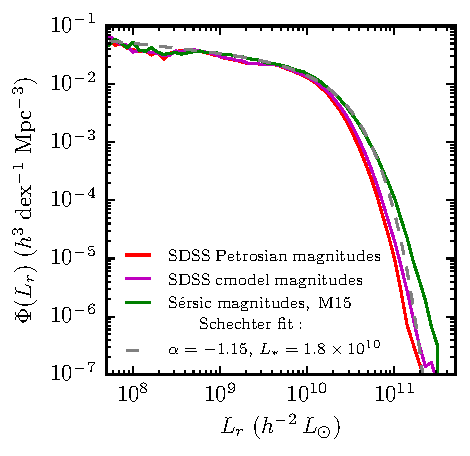
\includegraphics[scale=1.5]{fig/lf_magdefs.pdf}}
\caption{ Galaxy luminosity functions for different magnitude definitions in the SDSS main galaxy sample. The solid red and magenta lines are luminosity functions, in which luminosities were computed using the Petrosian and cmodel magnitudes, respectively, without $K$-correction. The solid green line is the luminosity function, in which magnitudes were computed using improved photometry based on the S\'ersic profile fits by \protect\href{http://adsabs.harvard.edu/abs/2015MNRAS.446.3943M}{\citet{meert_etal15}} where galaxy luminosites were $K$-corrected. The gray dashed line shows the best fit Schechter function for the latter LF with the best fit faint-$L$ slope and characteristic luminosity (in $h^{-2}\, L_{\odot}$) given in the legend. \label{fig:lfmagdefs}}
\end{figure}

{\it The $1/V_{\rm max}$ method}.  Maarten Schmidt is famous for discovering an interpretation of spectra of quasars as high redshift objects. A few years after this discovery, when the sample of quasars became sufficiently large, he estimated the luminosity function of quasars (see the beginning of Section VII on p. 403 in \href{http://adsabs.harvard.edu/abs/1968ApJ...151..393S}{\citep{schmidt68}}) using a simple method to correct for the Malmquist bias: instead of counting each quasar with an equal weight, thereby overweighing luminous quasars due to the larger volume to which they are detectable in a given survey, objects were counted by first calculating the maximum distance at which they could be seen given the survey limit, finding the volume of a sphere of this radius (the so-called $V_{\rm max}$) and then weighting the count by the inverse of this volume.

More precisely, continuing with the notion of the luminosity function as a histogram, in this method we construct a weighted histogram with weights $1/V_{\rm max}(L)$, where $V_{\rm max}(m_{\rm lim},L)$ is the maximum {\it comoving\/} volume to which a given object of luminosity $L$ will be visible given the apparent magnitude limit $m_{\rm lim}$ of the sample. It is clear that this method assumes that galaxies are distribured uniformly in space, which, as we saw, is not strictly true due to sample variance. Thus, the $1/V_{\rm max}$ method estimate of the LF is approximate and is often accompanied by additional corrections (e.g., \href{http://adsabs.harvard.edu/abs/2012MNRAS.421..621B}{\citealt{baldry_etal12}}, \href{http://adsabs.harvard.edu/abs/2015ApJ...803...34B}{\citealt{bouwens_etal15}}) that
 improve upon the method $1/V_{\rm max}$ by splining or binning variations of galaxies with redshift and then dividing the LF by a correction factor based on these variations. \href{http://adsabs.harvard.edu/abs/1977AJ.....82..861F}{\citet{felten77}} presents detailed analysis of the $1/V_{\rm max}$ estimator of the luminosity function in practice and some of the associated issues. 
 
Note that the $1/V_{\rm max}$ can be used not just to estimate the galaxy luminosity function, but more generally as a way to represent galaxies of different luminosities with correct relative weights in a histogram constructed from a flux-limited sample. We will be using it for such purposes below. 

Figure \ref{fig:lfmagdefs} shows the luminosity function of galaxies in the SDSS main spectroscopic sample for different ways of measuring apparent magnitudes of galaxies. 
The solid red and magenta lines are luminosity functions, in which luminosities were computed using the Petrosian and cmodel magnitudes estimated by the SDSS pipeline as described above (see also \S \ref{sec:petromagsize} and \ref{sec:cmodelmag}), respectively, without $K$-correction. The solid green line is the luminosity function, in which luminosity functions were computed using improved photometry based on the S\'ersic profile fits by \protect\href{http://adsabs.harvard.edu/abs/2015MNRAS.446.3943M}{\citet{meert_etal15}} where galaxy luminosites were $K$-corrected. 
It is clear that the bright end of the luminosity function is quite sensitive to how magnitudes are estimated (see, \href{http://adsabs.harvard.edu/abs/2013MNRAS.436..697B}{\citealt{bernardi_etal13}} for a more detailed discussion). One should be aware of this dependence when comparing theoretical models of galaxy evolution to observational estimates of the luminosity function or the stellar mass function derived from it.

The gray dashed line in Figure \ref{fig:lfmagdefs} shows the best fit Schechter function for the LF estimated from S\'ersic fit photometry. Overall, it provides a reasonable fit for $L_r\lesssim 10^{11}h^{-2}\, L_{\odot}$. The best fit has a faint-end slope of $\alpha\approx -1.2$ and a characteristic luminosity (at which number density of galaxies starts to fall of exponentially) of $L_{\ast,r}\approx 2\times 10^{10}\, h^{-2}\, L_{\odot}$, roughly consistent with other recent measurements. There is an ongoing debate about the correct slope of the luminosity function at low luminosities. This is because galaxies at these $L$ are dominated by low-surface brightness systems, as the mean surface brightness decreases with decreasing luminosity (see below). A given galaxy survey may thus be increasingly incomplete with decreasing $L$ thereby underestimating $\alpha$. A recent measurement of the luminosity function using the GAMA survey -- a survey that sampled a smaller volume survey, but going deeper to fainter luminosities and lower surface brightnesses than the SDSS main galaxy sample -- indicates a steeper faint end slope of $\alpha\approx -1.5$ \href{http://adsabs.harvard.edu/abs/2012MNRAS.421..621B}{\citep{baldry_etal12}}. 

At large luminosities a Schechter fit underestimates the measured LF. For greater flexibility, the sum of two or three Schechter functions is often used to model the LF (e.g., \href{http://adsabs.harvard.edu/abs/2009MNRAS.398.2177L}{\citealt{li_white09}}). Sometimes the Schechter function is modified to the following more flexible form (e.g.,  Eq.~9 in \href{http://adsabs.harvard.edu/abs/2010MNRAS.404.2087B}{\citealt{bernardi_etal10}}):
\begin{equation}
\phi(L)\equiv\frac{dn(L)}{dL}=\frac{\phi_*}{L}\frac{\beta}{\Gamma(\alpha/\beta)} \left(\frac{L}{L_*}\right)^{\alpha}\exp(-[L/L_*]^\beta),
\label{eq:lfLschechtermod}
\end{equation}
where $\Gamma(x)$ is the gamma function and $\beta$ is additional parameter that provides more flexibility at high luminosities. Some studies use sums of such modified Schechter funcitons to model the luminosity function. Another model often encountered is modified form above but with a broken power law at faint luminosities (\href{http://adsabs.harvard.edu/abs/2005ApJ...631..208B}{\citealt{blanton_etal05}}).

%-----------------------------------------------
\section{Galaxy spectra and colors}
%-----------------------------------------------

The color of an astronomical object is defined as the difference in apparent magnitudes between two spectral bands defined by two different filters. It is thus a quantity that depends on the specific choice of filters. The color also depends on how magnitudes 
are defined and are thus specific to a given magnitude system and method used to measure magnitudes.  For example, Figure \ref{fig:gal_spectra} shows several representative examples of SDSS galaxies of different colors ranging from blue ($g-r\approx 0.3-0.5$) to green ($g-r\approx 0.55-0.7$) and red ($g-r> 0.7$).  The right panels show
the corresponding spectra across the SDSS filter range. The legend in the upper right corner shows the $(g-r)$ color of each galaxy computed using the Petrosian magnitudes of the SDSS catalog in the corresponding bands. However, if we attempt to compute this color directly from the spectrum using equation \ref{eq:magforcolor} above, we find a color that is redder by $\approx 0.1-0.2$ magnitudes, especially for the late type galaxies. This is because the spectra are measured from the region of $1.5^{\prime\prime}$ radius around the center (the radius of the SDSS fiber), while the magnitudes are measured by integrating most of the light in each galaxy. The difference in color between the nuclei and outskirts of galaxies is visually apparent in the images of spiral galaxies in the left column of Figure \ref{fig:gal_spectra}.

\begin{figure}[!ht]
\centerline{
\includegraphics[scale=1.2]{fig/gal_img_spec_[1237668297144926308].pdf}}
\vspace{-3mm}
\centerline{
\includegraphics[scale=1.2]{fig/gal_img_spec_[1237662307800842404].pdf}}
\vspace{-3mm}
\centerline{
\includegraphics[scale=1.2]{fig/gal_img_spec_[1237659132751577202].pdf}}
%\centerline{
%\includegraphics[scale=.9]{fig/gal_img_spec_1237668623557394652.pdf}}
\caption{Examples of nearby SDSS galaxies of different $(g-r)$ color. Left column shows images of galaxies, while the right column shows  spectra of these galaxies. The shaded regions are the sensitivity curves of the SDSS filters. \label{fig:gal_spectra}}
\end{figure}

\begin{figure}[t]
\centerline{
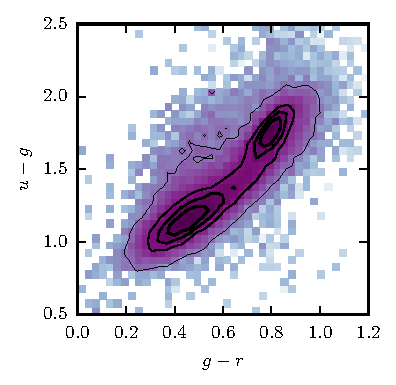
\includegraphics[scale=2.0]{fig/grug.pdf}}
\caption{The distribution of galaxies with $r$-band absolute magnitude $M_r<-19$ in the color-color plane of $g-r$ and $u-g$ colors. The galaxies were selected within $200h^{-1}$ Mpc and represent a volume-limited sample. The distribution of galaxies is not uniform, but is characterized by blue and red clumps with a ``green valley'' between them. \label{fig:gal_colcol}}
\end{figure}


\begin{figure}[!ht]
\centerline{
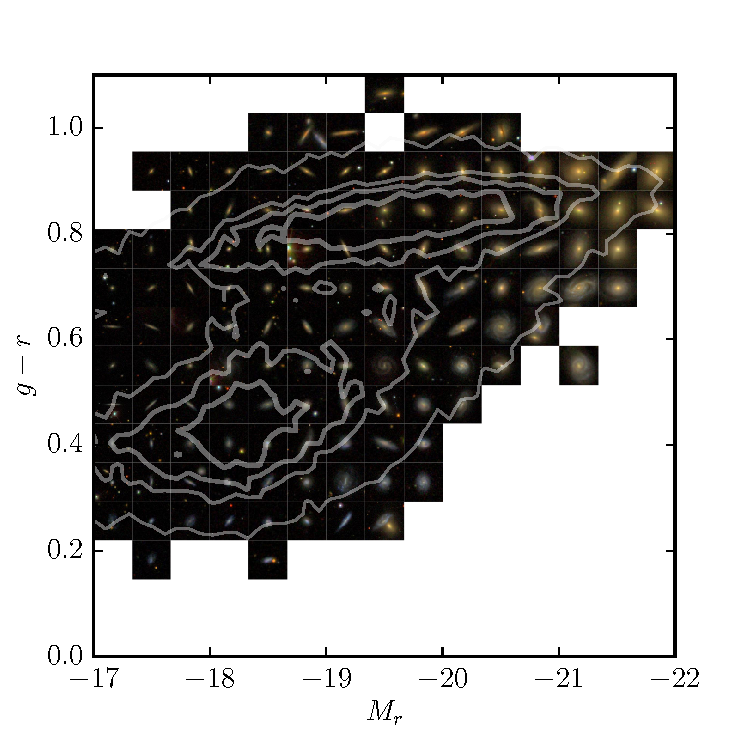
\includegraphics[scale=1.3]{fig/Mrgr_collage.pdf}}
\vspace{-5mm}
\caption{The contours show the distribution of SDSS galaxies within $150h^{-1}$ Mpc in the $M_r$ and $g-r$ plane. In the background is a collage of images of galaxies randomly selected from within the corresponding magnitude and color bins. Each image shows a region of $25h^{-1}$ kpc. The four contours enclose 95\%, 70\%, 45\% and 20\% of all galaxies.The distribution of galaxies is not uniform, but is characterized by a blue clump, a red sequence, and a ``green valley'' between them. Note that within the selection volume the sample is not complete for galaxies with $M_r> -18.5$. Thus, the actual fraction of galaxies in the blue clump is larger than indicated by this plot. \label{fig:Mrgr_collage}}
\end{figure}

Figure \ref{fig:gal_spectra}  also shows that the spectra clearly change qualitatively between blue and red galaxies. Blue and green galaxies have rather flat continua, prominent narrow emission lines, and only weak absorption lines. Red galaxies have spectra with suppressed emission in the $u$ and $g$ bands, do not have strong emission lines, and strong absorption lines and bands. 

A rough characterization of these spectral shapes can be captured by colors defined using different bands. Figure \ref{fig:gal_colcol} shows the distribution of galaxies of $r$-band absolute magnitude $M_r<-19$ in the color-color plane of $g-r$ and $u-g$ colors. The galaxies were selected within $200h^{-1}$ Mpc and represent a volume-limited sample. The figure clearly shows that the distribution of galaxies is not uniform, but is characterized by blue and red clumps with a ``green valley'' between them at
$u-g\approx 1.5$ and $g-r\approx 0.7$.

Figure \ref{fig:Mrgr_collage} shows the  distribution of galaxy $g-r$ color as a function of galaxy $r$-band absolute magnitude, $M_r$, along with a grid of postage stamp images of randomly selected galaxies in  $M_r-(g-r)$ bins. The blue clump and elongated ``red sequence'' of galaxies are clearly visible. Galaxies with luminosities $M_r>-20.5$ span a wide range of colors, although the faintest galaxies have mostly blue colors. The brightest galaxies are predominantly red and have mostly early morphological types.

\subsection{$k$-correction}

When we study the properties of galaxies from a wide range of redshifts in a given band, we are actually studying different, coarsely binned, parts of their spectra. For example, if the
spectrum of a galaxy is steeply falling towards bluer wavelengths in roughly the same range as a given filter, a larger redshift will cause a galaxy of constant luminosity to appear dimmer just due to the filter response sliding
down the spectrum. We are usually interested in the actual physical evolution of galaxy luminosities, not in the artificial effects of a limited filter range.
To correct for this filter-induced evolution, one applies the so-called $k$-correction to the luminosity measured in a given band (see \href{http://adsabs.harvard.edu/abs/1968ApJ...154...21O}{\citealt{oke_sandage68}} and \href{http://adsabs.harvard.edu/abs/2002astro.ph.10394H}{\citealt{hogg_etal02}}) using equation \ref{eq:kcorr} in \S \ref{sec:mML}.

Given that galaxy spectra differ for different types of galaxies, $k$-correction is spectrum dependent. The correction is applied broadly to spectra with similar shapes, as quantified by broadband colors. The principle is thus simple, although in practice there are many
subtleties (see, e.g., \href{http://adsabs.harvard.edu/abs/2007AJ....133..734B}{\citealt{blanton_roweis07}}). For example, we cannot just use the SDSS spectra to measure the $k$-correction for a given galaxy 
because spectra are taken through fibers of limited aperature and reflect the color of the region within that aperture, which can be significantly different from the 
spectrum of the entire galaxy. Also, the spectra of particular galaxies may be subject to observational limitations, such as limited wavelength range. 

Thus, in practice sophisticated modelling of $k$-correction employing well-determined characteristic spectral templates is used. A widely used example is the the $k$-correction model of \href{http://adsabs.harvard.edu/abs/2007AJ....133..734B}{\citet{blanton_roweis07}} implemented in the \href{http://cosmo.nyu.edu/mb144/kcorrect/v3_2-index.html}{{\tt kcorrect} code}.  At the same time, simple approximations exist for $k$-correction (\href{http://adsabs.harvard.edu/abs/2010MNRAS.405.1409C}{\citealt{chilingarian_etal10}}, \href{http://adsabs.harvard.edu/abs/2012MNRAS.419.1727C}{\citealt{chilingarian_zolotukhin12}}) with an online calculator and code snippets available \underline{\href{http://kcor.sai.msu.ru/}{here}}. The effect of $k$-correction on luminosity of bright red galaxies with a typical red color ($g-r=0.8$) can be gleaned from the difference between dark orange and yellow lines in Figure \ref{fig:Mzsdss}. The effect is quite small at $z<0.3$ compared to the effects of photometry method or galaxy evolution over this redshift interval. At higher redshifts, however, effects of $k$-correction grow larger and it can be a source of significant systematic error in measurements of galaxy luminosities and luminosity functions (e.g., \href{http://adsabs.harvard.edu/abs/2016arXiv160307299L}{\citealt{lake_wright16}}).

\begin{figure}
\centerline{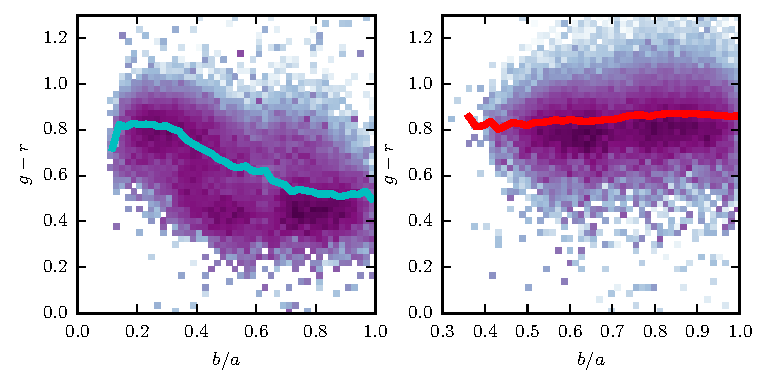
\includegraphics[scale=1.3]{fig/bagr_dust_meert.pdf}}
\caption{The $g-r$ color of late (left) and early (right) type galaxies as a function of the axis ratio of and ellipsoidal fit to the galaxy's light. Smaller axis ratios correspond to more flattened systems viewed closer to the edge-on view.  The color maps show the distribution of galaxies of $M_r<-19$ in the \href{http://adsabs.harvard.edu/abs/2015MNRAS.446.3943M}{\citet{meert_etal15}} catalog. 
The distribution in the left panel includes only the galaxies with probability to have late type in the classification of \protect\href{http://www.aanda.org/articles/aa/abs/2011/01/aa15735-10/aa15735-10.html}{\citet{huertas_company_etal11}} of $>0.7$, while in the right plot distribution includes galaxies with the probability to be elliptical or S0 of $>0.7$.  The lines in both panels show median $g-r$ at a given $b/a$.
The plot shows that highly inclined, nearly edge-on disk galaxies have $g-r$ colors that are $\approx 0.3$ redder on average than disks viewed face on. The effect on blue-band colors, such as $u-g$ or $u-z$ will be even larger because dust affects bluer wavelengths more strongly. The right panel shows that there is no trend of color with axis ratio for the early type galaxies. Note that the range of axis ratios shown in the right panel is smaller because distribution of $b/a$ of these galaxies does not extend to $<0.4$. Note also the paucity of disks with $a/b<0.1$ in the left panel.  \label{fig:colorinc}}
\end{figure}

\subsection{Interpretation of galaxy spectra}

Comparisons of the spectra in Figure \ref{fig:gal_spectra}  with the spectra of stars of different classes \citep[see, e.g., spectra in][]{jacoby_etal84} shows that the spectra of blue and green galaxies are dominated by young and intermediate age stars (which have hot atmospheres with relatively weak absorption), while the spectra of red galaxies are similar to those of K class stars. This class ranges from faint small mass stars to stars along the red giant (RG) and asymptotic giant branch (AGB). The latter usually dominate the light and the spectrum of their host galaxy. Stars do not produce emission lines. These come from interstellar gas, in which atoms are excited by energetic UV radiation and re-radiate it in the lines corresponding to their electron energy levels. UV photons are produced predominantly by young stars \footnote{Some UV photons may be produced by stars in advanced stages of evolution, but at a much lower level} and thus these emission lines indicate both the recent star formation and the presence of fuel for continuing star formation in the form of gas. 
%{\bf Add plot of spectra for stars of different types from SDSS.}

%------------------------------------------------------
\subsection{Stellar population synthesis}
\label{sec:SPSoverview}
%------------------------------------------------------

While there is some qualitative similarity between galaxy spectra and the spectra of stars of particular spectral classes, these spectra are also noticeably different, especially 
for bluer galaxies. This is because the spectra of galaxies are actually a combination of spectra of stars of different mass, metallicity, and evolutionary stage. In galaxies with gas and dust, gas emission contributes to the overall spectrum and dust affects the spectrum by preferentially scattering light at bluer wavelengths.  

It is all but impossible
to decompose a spectrum into properties of individual stars due to our limited knowledge of the star formation history, metallicity distribution, initial mass function, etc., of a given galaxy. So 
spectra are typically forward modelled by making simplifying assumptions about these properties in {\it the stellar population synthesis} (SPS) models \citep[see][for a recent in depth review]{conroy13}. The key assumptions that need to be made and which are the main source of uncertainty are the initial stellar mass function (IMF) of stars and star formation history (SFH) of a galaxy. There is no solid theory that predicts these and, while there is data on both the IMF and SFHs, the empirical information and guidance in modelling that it can provide are limited. Additional uncertainties are introduced by models of stellar evolution, dust, etc.

Nevertheless, SPS modelling is a powerful and very useful tool. It is not in widespread use in galaxy studies. Perhaps the most common use is to convert luminosities into stellar masses using galaxy spectra or colors using SPS estimates of the stellar mass to light ratio, $M_*/L$: $M_*=(M_*/L)\times L$.  
An estimate of $M_*/L$ can be obtained with an SPS model given assumptions described above for a galaxy with a given spectrum, because such model can be used derive the best fit estimate of the stellar population properties, including stellar mass and metallicity that produces a galaxy with a given luminosity in different bands. 

These models predict that mass-to-light ratios are particularly simple linear functions of galaxy colors (e.g., \href{http://adsabs.harvard.edu/abs/2003ApJS..149..289B}{\citealt{bell_etal03}}, \href{http://adsabs.harvard.edu/abs/2009MNRAS.400.1181Z}{\citealt{zibetti_etal09}}) -- the fact that is used extensively for crude conversions of luminosities into stellar mass. For example, calculations of \href{http://adsabs.harvard.edu/abs/2003ApJS..149..289B}{\citet{bell_etal03}} predict that for a galaxy with a given $g-r$ color, the mass-to-light ratio in the $r$-band is: $\log_{10}(M_*/L_r)=-0.305+1.097\times (g-r)$, where $M_*$ is in $M_\odot$ and $L_r$ is in $L_\odot$. For similar calibrations for other bands and colors see their Appendix A.2 and Table 7. Note, however, that in reality there is substantial scatter around these relations and their exact form depends on assumptions of the SPS modelling. Thus, they should be treated as fairly crude approximations, not precise predictions (despite the large number of significant digits provided in the fit parameters).

\subsection{Dust reddening}

Figure \ref{fig:colorinc} shows the colors of SDSS galaxies as a function of their apparent ellipticity characterized by the axis ratio of their light distribution. The left and right panels show distribution for galaxies classified as disks and early type (E+S0). Namely, they have probabilities to be in these classes of larger than $0.7$ in the classification of  \href{http://www.aanda.org/articles/aa/abs/2011/01/aa15735-10/aa15735-10.html}{\citet{huertas_company_etal11}}. The figure shows a clear trend of increasing color (i.e., reddening) with decreasing $b/a$ for disk galaxies, but no trend for early type galaxies. 

From examining galaxy images we know that disks viewed edge on often have reddish ``dust lanes.'' It is the dust within the disk that creates these lanes and causes reddening of color.\footnote{Note that the SDSS magnitudes are already corrected for the foreground reddening and extinction within our own Galaxy. Here we talk about reddening due to dust internal to each specific galaxy.} As $b/a$ decreases the path length and total column density of dust through the disk increases as well reddening colors. The dust reddening is one of the main reasons why many galaxies with disk morphologies can be found among galaxies in the red sequence. A disk may also be red if its stellar population is dominated by genuinely old stars. However, as can be clearly seen in 
Figure \ref{fig:colorinc}, the dust reddening is a large effect and is the main factor determining red color for many disks (see \href{http://adsabs.harvard.edu/abs/2007MNRAS.379.1022D}{\citealt{driver_etal07}}, \href{http://adsabs.harvard.edu/abs/2008ApJ...687..976U}{\citealt{unterborn_ryden08}}, \href{http://adsabs.harvard.edu/abs/2009ApJ...691..394M}{\citealt{maller_etal09}} for in-depth studies of such reddening). 

Dust absorbs bluer light much more and so colors involving blue bands are more affected. For some highly inclined galaxies dust may affect bluer bands by as much as $\sim 1.5$ magnitudes \citep{driver_etal07,maller_etal09}. This means that to get accurate {\it intrinsic} properties of disk galaxies, such as color (and spectrum) we need to correct for dust effects using inclination information, which can be done by shapes that are derived using information from the near infrared that is less affected by dust \citep{maller_etal09}. Apparently, dust lanes almost entirely disappear for dwarf galaxies with rotation velocities $<120$ km/s \href{http://adsabs.harvard.edu/abs/2006AJ....131..226Y}{\citep{yoachim_dalcanton06}}.  

Elliptical galaxies have almost no cold ISM and little dust (although they do have some) and thus they do not suffer from the same inclination effects, as can be seen in the right panel of Figure \ref{fig:colorinc}. In addition, the dust distribution in spheroidal galaxies probably does not correlate with the axis ratio of stellar distribution, which is determined not by rotation but by the velocity anisotropy tensor. 

\begin{figure}[!ht]
\centerline{
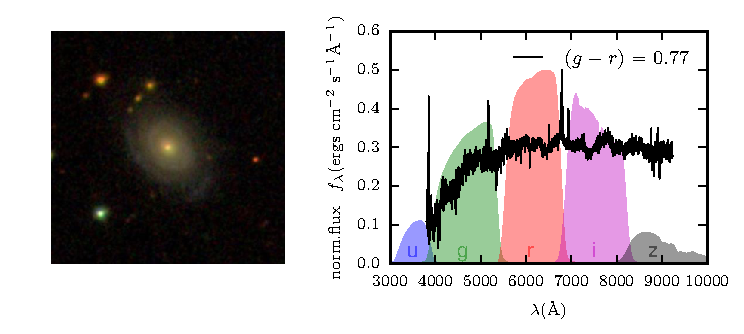
\includegraphics[scale=1.25]{fig/gal_img_spec_1237665369572376858.pdf}}
\centerline{
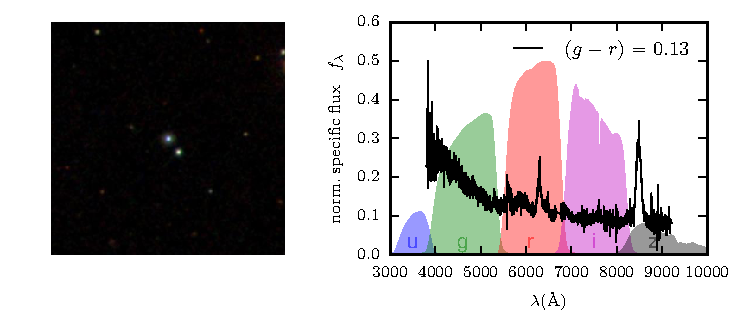
\includegraphics[scale=1.25]{fig/gal_img_spec_1237662335719833753.pdf}}
\vspace{-5mm}
\caption{Top panels: the image and spectrum of a galaxy spectrum superimposed with the spectrum of the AGN in its center. Bottom panels: the image and spectrum of a quasar. It looks like a star in the image, but has a completely non-stellar spectrum. \label{fig:AGN_spectra}}
\end{figure}

\section{Active Galactic Nuclei}

In galaxies with active galactic nuclei (AGN), emission from gas in and near black hole accretion disk is super-imposed on the rest of galaxy spectrum (see Fig. \ref{fig:AGN_spectra}).  In the case of low-luminosity AGNs, the emission from AGN's circum-black hole region can contribute significant, but minor fraction of the total galaxy light. However, in the case of quasars, the AGN emission  
can completely dominate over the luminosity of its host galaxy, such that galaxy light can only be uncovered in high-quality data and even then only after applying a sophisticated analysis (e.g., \href{http://adsabs.harvard.edu/abs/1999ApJ...520...67K}{\citealt{kirhakos_etal99}}). 

Given that regions contributing to AGN emission are small ($<1\ \rm pc$), they are unresolved in images and appear point- or star-like. Their spectra, however, have strong and often broad emission lines and are thus unlike spectra of any stars (see an example in the bottom panels of Fig. \ref{fig:AGN_spectra}). Historically, 
such {\it quasi-stellar objects} (QSOs) were discovered as radio sources, which in the visible wavelengths appeared as star-like objects with unusual spectra. Their spectra and lines were a mystery until Maarten Schmidt figured out that the lines in the spectrum of one of such objects, 3C273, were well-known transitions just red-shifted by an unusually large amount\footnote{Unusually large for that time, at least. See \href{http://www.annualreviews.org/doi/abs/10.1146/annurev-astro-082214-122514}{\citet{schmidt15}} for a biographical account by Maarten Schmidt of this discovery.} \href{http://adsabs.harvard.edu/abs/1963Natur.197.1040S}{\citep{schmidt63}}. 


\begin{figure}[t]
\centerline{
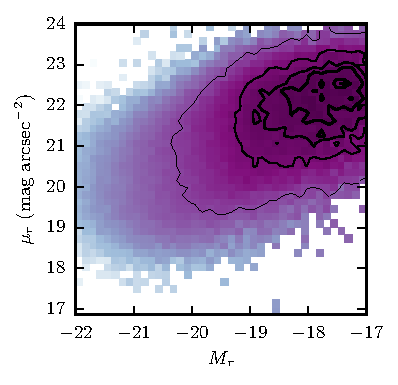
\includegraphics[scale=2.0]{fig/Mrmur.pdf}}
\caption{The distribution of the $r$-band surface brightness of SDSS galaxies, $\mu_r$, as a function of their absolute $r$-band magnitude, $M_r$.   We can see a systematic trend of increasing surface brightness with increasing luminosity. The distribution was corrected for the Malmquist bias using the $1/V_{\rm max}$ weighting. \label{fig:Mrmur}}
\end{figure}



\section{Structural properties of galaxies and their relation to morphology}

We have already considered surface brightness profiles and saw that they can be described by the S\'ersic profile with a range of indices $n$. We also discussed that galaxies often exhibit indications of multiple components in the distribution of light. Here we will discuss simple quantities parametrizing basic properties of light distribution and their relation to morphology. 

\subsection{Galaxy surface brightness}

Let us return to Figure \ref{fig:Mrgr_collage} showing images of representative galaxies in the $M_r-(g-r)$ plane. Recall that each postage stamp image in the grid shows a region of the same physical size of $25h^{-1}$ kpc. Thus, the relative sizes of galaxies are represented correctly. One can see from the 
figure that the physical size of galaxies correlates with its luminosity. We will examine this correlation in more detail later, but for now note that for faint galaxies correlation is actually quite weak (if present at all).

As we discussed above, surface brightness is defined as the amount of light that we receive from a given area of the galaxy. This quantity makes sense for an extended object. It can be defined for example using the total magnitude or luminosity computed within a given filter using one of the methods discussed above and the radius enclosing half of this total light. So, if the total luminosity is $L$ and half-light radius is $R_{1/2}$, we can define galaxy surface brightness as $\Sigma=L/(2\pi R_{1/2}^2)$.  One can also use stellar population modelling of galaxy colors or spectra to derive underlying stellar mass under the model assumptions. Thus, sometimes we use total stellar mass $M_\ast$ in lieu of $L$, in which case we talk about stellar {\it surface density.}

 The weak correlation of size with luminosity means that for galaxies of increasing luminosity, size increases slowly and so {\it surface brightness} increases with increasing galaxy luminosity. Conversely, fainter galaxies tend to have lower surface brightness. This is illustrated in Figure \ref{fig:Mrmur}, which shows distribution of the $r$-band surface brightness as a function of $M_r$ for SDSS galaxies. The figure shows a strikingly large variation of surface brightnesses of galaxies of a given absolute magnitude. 

Historically, it was believed that early type galaxies tend to have a narrow range of high values of the {\it central\/} surface brightnesses, which is sometimes called the "Kormendy law" \href{http://adsabs.harvard.edu/cgi-bin/bib_query?1977ApJ...218..333K}{\citep{kormendy77}}, while the tendency of for late type galaxies to concentrate near the peak of the low-concentration clump is called the "Freeman law" \href{http://adsabs.harvard.edu/cgi-bin/bib_query?1970ApJ...160..811F}{\citep{freeman70}}. Specifically,  \href{http://adsabs.harvard.edu/cgi-bin/bib_query?1970ApJ...160..811F}{\citet{freeman70}} found that the central surface brightnesses of spiral galaxies in the $B$-band occupied a narrow range: $\mu_{\rm B}\approx 21.6\pm 0.3\ \mathrm{mag\ arcsec^{-2}})$. As can be seen from Figure \ref{fig:Mrmur}, large galaxy surveys showed that these "laws" simply reflect the tip of the iceberg of the surface brightness distributions of late and early type galaxies. The overall population exhibits a much wider range of surface brightnesses. 

The actual distribution may be even wider than Figure \ref{fig:Mrmur} indicates, especially for low luminosity galaxies. This is because a population of {\it low-surface brightness} (LSB) galaxies is missing in them. Such galaxies form a tail of the distribution of late type galaxies towards surface brightnesses dimmer than the "blue island" of late type galaxies and are particularly abundance at faint magnitudes (\href{http://adsabs.harvard.edu/abs/1997PASP..109..745B}{\citealt{bothun_etal97}}, \href{http://adsabs.harvard.edu/abs/2004PASA...21..344D}{\citealt{driver04}}). You can see the distribution of surface brightnesses as a function of galaxy luminosity (expressed as absolute magnitude) \href{http://ned.ipac.caltech.edu/level5/Sept04/Driver/Figures/figure2.jpg}{\underline{here}}.

The LSB galaxies have disk or irregular morphologies. However, they are difficult to detect against the brightness of the night sky and are thus largely missing in galaxy surveys unless a special care is taken to include them as is done in some special deep surveys (e.g., \href{http://adsabs.harvard.edu/abs/2005MNRAS.360...81D}{\citealt{driver_etal05}}). 

One striking manifestation of this difficulty is reflected by the fact that we are still discovering copious numbers of new satellite galaxies of the Milky Way (\href{http://adsabs.harvard.edu/abs/2015ApJ...805..130K}{\citealt{koposov_etal15}}, \href{http://adsabs.harvard.edu/abs/2015ApJ...813..109D}{\citealt{drlica_wagner_etal15}}). Very diffuse, low-surface brightness galaxies are also being discovered in significant numbers at larger distances (\href{http://adsabs.harvard.edu/abs/2015ApJ...798L..45V}{\citealt{vandokkum_etal15}}).

\begin{figure}[!th]
\centerline{
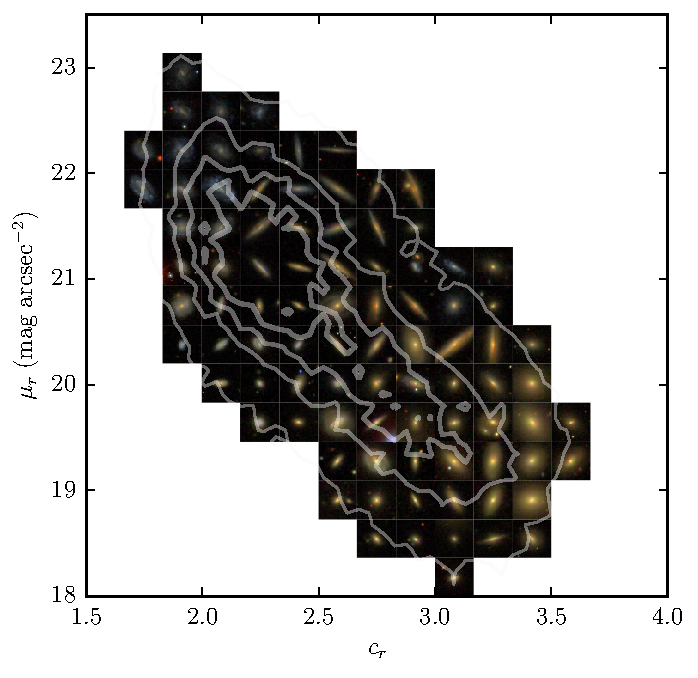
\includegraphics[scale=1.2]{fig/crmur_collage.pdf}}
\caption{Contours show the distribution of SDSS galaxies in the plane of light concentration vs the $r$-band surface brightness. In the background a grid of postage stamp images of randomly selected galaxies in bins of $c_r$ and $\mu_r$ are shown for illustration. Each image shows a region of $25h^{-1}$ kpc. The four contours enclose 95\%, 70\%, 45\% and 20\% of the galaxy distribution. The distribution of galaxies is not uniform, but is characterized by two clumps of low and high concentration and surface brightness. These clumps reflect bi-modality in the {\it structural} properties of galaxies and are thus qualitatively different from the bimodality and color in Figure \ref{fig:Mrgr_collage}. \label{fig:crmur_collage}}
\end{figure}

\begin{figure}[!th]
\centerline{
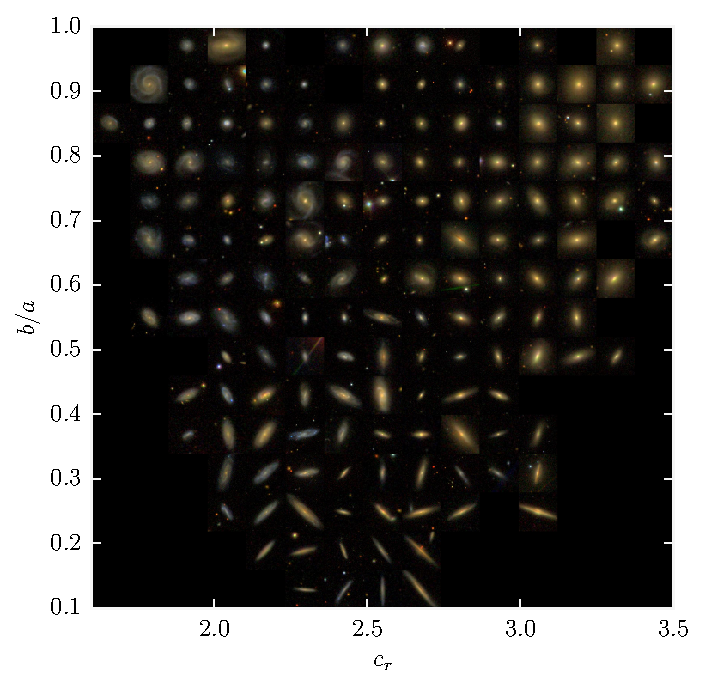
\includegraphics[scale=1.4]{fig/crab_collage.pdf}}
\vspace{-5mm}
\caption{Collage of images of the SDSS galaxies randomly drawn from the sample of galaxes with $M_r<-19$ at distances $d_L<200$ Mpc in the concentration--image axes ratio plane $c_r-b/a$. The figure shows that different morphological types separate well in this plane: late type close to face-on galaxies occupy upper left corner of the distribution, elliptical galaxies are in the upper right corner, edge-on disks are in the bottom--center, and lenticular galaxies occupy the middle--right part of the diagram.\label{fig:crba_collage}}
\end{figure}



\begin{figure}[!ht]
\centerline{
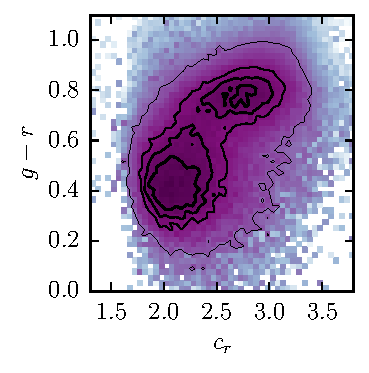
\includegraphics[scale=2.2]{fig/cr_gr.pdf}}
\vspace{-5mm}
\caption{Distribution of galaxies of in the $r$-band concentration, $c_r$, $g-r$ color plane. Galaxies are weighted by their $1/V_{\rm max}$ to remove the Malmquist bias. The four contours enclose 95\%, 70\%, 45\% and 20\% of the galaxy distribution. 
The distribution of galaxies is not uniform, but is characterized by two clumps. We have previously seen bimodality of color (the quantity controlled by age of stellar population, its metallicity, and affected by dust reddening), this plot indicates that there is also a weaker bimodality in the concentration of
light distribution -- a property describing structure of galaxies. 
\label{fig:gal_crgr}}
\end{figure}
\subsection{Light concentration}

Another simple quantity that can be defined without knowledge of galaxy distance, is the {\it concentration of its light distribution}. SDSS database provides estimates of the radii (in arcsec) enclosing 50\% and 90\% of the total light estimated using the  \href{http://adsabs.harvard.edu/cgi-bin/nph-bib_query?bibcode=1976ApJ...209L...1P}{\citet{petrosian76}} method (see Appendix \ref{sec:petromagsize}). Their {\it ratio\/} provides us with a distance-independent measure of  concentration of galaxy light:\footnote{For distant galaxies of $R_{50}\lesssim 3^{\prime\prime}$ concentration is affected by seeing to some extent - see \href{http://adsabs.harvard.edu/abs/2003ApJ...594..186B}{\citet{blanton_etal03}}. This is not a significant worry for our broad brush estimates, although if working with sufficiently large sample cuts on size to $>3^{\prime\prime}$ are prudent.}
\begin{equation}
c\equiv R_{90}/R_{50}.
\label{eq:cpetr}
\end{equation}
 For example, if galaxy light is redistributed in such a way that more of it is concentrated towards the center, $R_{90}$ should be largely unaffected, while $R_{50}$ should decrease and thus $c$ would increase.
 \href{http://adsabs.harvard.edu/abs/2001AJ....122.1861S}{\citet{strateva_etal01}} showed that this concentration tightly correlates with the traditional morphological types of galaxies obtained via visual classification. 

It may seem like concentration is similar to surface brightness, but they are actually distinct properties: 
concentration can be thought of as parametrizing shape of the luminosity profile, while surface brightness quantifying its normalization. In practice, however, the two quantities are correlated. 
Figure \ref{fig:crmur_collage} shows the distribution of galaxies in the $c_r$-$\mu_r$ plane along with randomly selected postage stamp images of galaxies in bins. The distribution is broad but exhibits a clear correlation between the two quantities. We can see that early type galaxies mostly populate the high concentration, high surface brightness end of the distribution, while the late type spirals occupy the low-concentration, low surface brightness end. 

If we examine galaxies in the horizonthal rows of a given $\mu_r$ in Figure \ref{fig:crmur_collage}, we see  fairly uniform morphologies at low surface brightness, but a wide range at intermediate and high $\mu_r$ values. The surface brightness is thus not a good indicator of morphology on its own. 

If we consider vertical columns of galaxies at a given $c_r$, the morphological mix tends to be uniform, except at high concentrations, where elliptical and S0 galaxies are inter-mixed with disk systems. Note, however, that the disk systems at high $c_r$ are all highly inclined. 
This is because the apparent concentration of an exponential disk depends on the inclination under which the disk is viewed. Nearly edge-on disks have high concentrations and are thus located in the high-$c$ tail. 
We can see that concentration is a potentially good indicator of galaxy morphology, if we could correct for the effects of inclination on disk galaxy concentrations. This can be done by dividing concentrations by the function that describes the change of exponential disk concentration with inclination, as proposed by \href{http://adsabs.harvard.edu/abs/2008ApJ...681..225B}{\citet{bailin_harris08b}}. 

The good separation of galaxies in the axes ratio -- concentration plane is illustrated in the collage of randomly drawn images of SDSS galaxies from the sample with $M_r<-19$ and distances of $d_L<200$ Mpc in Figure \ref{fig:crba_collage}. The figure shows that different morphological types separate well in this plane: late type close to face-on galaxies occupy upper left corner of the distribution, elliptical galaxies are in the upper right corner, edge-on disks are in the bottom--center, and lenticular galaxies occupy the middle--right part of the diagram. 

This nice separation of types motivates the use of $b/a$ and $c_r$ with a machine learning classification method to classify galaxy morphogies. These methods work by first definition regions occupied by galaxies of different morphological classes given the training sample with known classes, and then classifying other galaxies of unknown class based on where they fall within the set of parameters on which training was performed. In this case, classification can be done using both $b/a$ and $c_r$, as well as other parameters correlating with morphology, such as color.

Figure \ref{fig:gal_crgr}, for example, shows distribution of $g-r$ color vs concentration, which features two distinct clumps of galaxies. We observed color bimodality before. However, here a bimodality in concentration is also present. This bimodality is in the {\it structural} property of galaxies and is thus qualitatively different from the bimodality of color.
For example, if a galaxy was building up its stellar mass at a steady rate, but color was changing nonlinearly with time due to peculiarities of shape evolution of stellar spectra with time, the bimodality of color could arise just from this nonlinearity. However, the fact that we see bimodality in the structural parameter in light distribution means that it reflects a real physical bifurcation of galaxy properties. In particular, this means that {\it galaxies become red when their light becomes concentrated due to some physical process.} 


\subsection{Vertical structure of disks}

Perpendicular to the plane disks are generally well described by an exponential atmosphere with a roughly isothermal profile at a given $R$, although the scale height varies with $R$ and disks often "flare" - increase scale height significantly in the outer regions. 
Figure \ref{fig:colorinc}) discussed above shows colors of SDSS disk galaxies as a function of their apparent ellipticity characterized by the axis ratio of light distribution. Smaller axis ratios correspond to more inclined disks. 
You can see that axis ratios are rarely less than 0.1. This reflects the finite thickness of the disks
in the direction perpendicular to the disk plane.  Indeed, a detailed study by \href{http://adsabs.harvard.edu/abs/2006AJ....131..226Y}{\citet{yoachim_dalcanton06}} shows that the ratio of the disk scale-length to the scale-height ranges in $\sim 8-12$ with a weak trend with galaxy mass and rotation velocity.

%--------------------------------
\section{Gas in galaxies}
\label{sec:gas}
%--------------------------------

Gas is a component of utmost importance in galaxies because it provides fuel for star formation and allows us to probe enrichment history and derive other useful information about galaxies. However, gas is also relatively difficult to observed compared to stellar light and thus less is generally known about gas content of galaxies, especially at higher redshifts.  

Recently, large surveys of galaxies have allowed studies of trends of gas content with galaxy properties to be studied in detail statistically at $z\sim 0$. For example, \href{http://adsabs.harvard.edu/abs/2011ApJ...732...93T}{\citet{toribio_etal11}} used the \href{http://egg.astro.cornell.edu/alfalfa/index.php}{ALFALFA 21-cm survey} to explore the multi-variate distribution of gas mass with other structural galaxy properties and the COLDGASS survey explored the trends of molecular gas mass fractions as a function of galaxy properties (\href{http://adsabs.harvard.edu/abs/2011MNRAS.415...32S}{\citealt{saintonge_etal11}}). 

Below we will review the main findings of such recent surveys. We will first consider the overall gas content of galaxies and then will consider radial distribution of gas in galaxies. 

\begin{figure}[t]
\centerline{
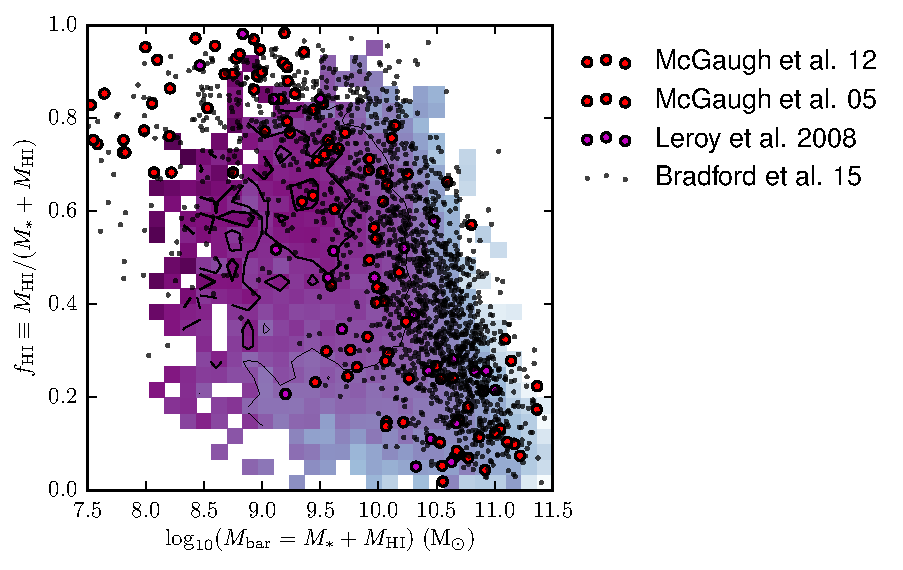
\includegraphics[scale=1.2]{fig/fgmb.pdf}}
\caption{Atomic gas mass fraction as a function of galaxy ``baryon mass'' approximated as a sum of stellar and HI gas mass. The points represent galaxies from various
observational samples (\href{http://adsabs.harvard.edu/abs/2012AJ....143...40M}{\citealt{mcgaugh_etal12}}, \href{http://adsabs.harvard.edu/abs/2008AJ....136.2782L}{\citealt{leroy_etal08}}, \href{http://adsabs.harvard.edu/abs/2015ApJ...809..146B}{\citealt{bradford_etal15}}), while the distribution shown by histogram and contours is constructed using galaxies from the \href{http://egg.astro.cornell.edu/alfalfa/index.php}{ALFALFA.40 survey} with identifiable optical counterparts in DR7. The galaxies in this distribution were weighted by $1/V_{\rm max}$ factor to correct for the Malmquist bias. \label{fig:fgmb}}
\end{figure}

\subsection{Atomic gas}

Figure \ref{fig:fgmb} shows the mass fraction of atomic HI gas versus  the sum of HI and stellar mass, $M_*$. The figure shows the overall trend of increasing gas fractions with decreasing baryon mass. The correlation is quite tight for massive galaxies, but scatter increases rapidly for dwarf galaxies. This large scatter at small masses was uncovered only recently with the advent of large HI surveys, such as \href{http://egg.astro.cornell.edu/alfalfa/index.php}{ALFALFA}, and dedicated surveys such as that by \href{http://adsabs.harvard.edu/abs/2012AJ....143...40M}{\citet{mcgaugh_etal12}},  \href{http://adsabs.harvard.edu/abs/2008AJ....136.2782L}{\citet{leroy_etal08}}, and \href{http://adsabs.harvard.edu/abs/2015ApJ...809..146B}{\citet{bradford_etal15}}. 
Comparison of points distribution to the histogram corrected for the Mamquist bias shows that the points tend to be distributed towards upper regions of the distribution of ALFALFA galaxies. This illustrates the effect of the Malmquist bias: the samples shown by points are dominated by more massive and gas rich galaxies at larger distances, and mis-represent the relative abundance of low-mass, low gas fraction galaxies. They also create an impression that correlation of gas fraction with $M_*+M_{\rm HI}$ is tighter than it actually is.

Note that for $M_{\mathrm{HI+\ast}}>10^9\ M_{\odot}$ there is a fraction of galaxies that have very little atomic gas. Some of these are spheroidal and lenticular galaxies, but many are disk galaxies. These are known as anemic or passive spirals (\href{http://adsabs.harvard.edu/abs/1976ApJ...206..883V}{\citealt{van_den_bergh76}}, \href{http://adsabs.harvard.edu/abs/2002AJ....124..777E}{\citealt{elmegreen_etal02}}).

At $M_{\mathrm{HI+\ast}}<10^9\ M_{\odot}$, however, all of the galaxies in various samples have $f_{\mathrm{HI}}>0.1-0.2$. This fact is probably related to the striking observation that {\it there are very few ($<0.06\%$) quenched (i.e., no longer star forming) galaxies in the field with $M_*<10^9\ M_{\odot}$} (\href{http://adsabs.harvard.edu/abs/2012ApJ...757...85G}{\citealt{geha_etal12}}). 


\subsection{Molecular gas}

 \href{http://adsabs.harvard.edu/abs/2011MNRAS.415...32S}{\citet{saintonge_etal11}} used the COLD GASS survey to show that there is an overall trend of mass fraction of gas in molecular form with galaxy stellar mass that can be approximated by: 
 \begin{equation}
 \log_{10}\chi_{\rm H_2}\equiv \log_{10}\left(\frac{M_{\rm H_2}}{M_{\rm HI}}\right)\approx -0.4\pm 1.5+(0.4\pm 0.1)(\log_{10}M_*-10.7).
\end{equation}
A trend with similar slope and scatter also exist as a function of stellar surface density within $R_{50}$, $\mu_{*,50}$. These trends were measured for galaxies with stellar masses $M_*\lesssim 10^{11}\ \rm M_\odot$ and will reverse for larger mass galaxies. Thus, the most massive elliptical galaxies, which have high surface densities, are typically deficient in both HI and H$_2$ gas.

The above relation imples that $L_*$ galaxies of the Milky Way mass ($\log_{10}M_*\approx 10.8$) near the knee of the luminosity function typically have molecular mass of $\approx 40\%$ that of HI: $\chi_{\rm H_2}\approx 0.4$. However, the uncertainties on the normalization of the relation above also indicates large scatter. Some galaxies have more molecular gas than HI, while others have molecular fractions considerably smaller than the mean. In the Milky Way, for example, $\chi_{\rm H_2}\approx 0.1$. Empirically, star formation in galaxies correlates strongly with the surface density and mass of molecular gas. Thus, scatter in the molecular gas content provides clues about different star formation rates in different galaxies. 

\subsection{Ionized gas}
Despite the fact that most of the baryons associated with disk galaxies are thought to exist in hot form in gaseous halo around the disk, remarkably little is known about these halos. From quasar absorption line studies, we know that the cricumgalactic gas is multi-phase. Hot, detailed structure of X-ray emitting halos around disk galaxies is largely still a terra incognita with only a handful of spirals with detections of diffuse X-ray emission (\href{http://adsabs.harvard.edu/abs/2013ApJ...772...97B}{\citealt{bogdan_etal13}}), although there are studies that showed regular correlations of X-ray luminosity with galaxy infrared luminosity (e.g., \href{http://arxiv.org/abs/1011.1906}{\citealt{crain_etal10}}). At the same time, the hot halos are expected to contain baryon mass comparable or larger than the mass of stars and gas in galaxies themselves. 

More recently, hot gas around bright galaxies was probed statistically via the Syunyaev-Zeldovich effect (\href{http://adsabs.harvard.edu/abs/2013A%26A...557A..52P}{\citealt{ade_etal13}}) and stacking of X-ray observations (\href{http://adsabs.harvard.edu/abs/2015MNRAS.449.3806A}{\citealt{anderson_etal15}}). These measurements show that bright galaxies are surrounded by extended halos of hot gas with properties consistent with extention of hot halos of galaxy groups and clusters. 

\begin{figure}[t]
\centerline{
\includegraphics[scale=.975]{fig/sgpro.pdf}\hspace{-2mm}\includegraphics[scale=.975]{fig/rsh_rgh.pdf}}
\vspace{-5mm}
\caption{Left panel: surface density profiles of atomic$+$ molecular gas in disk galaxies in the LITTLE THINGS sample of dwarf galaxies (\href{http://adsabs.harvard.edu/abs/2012AJ....143...47Z}{\citealt{zhang_etal12}}) and sample of disk galaxies of \href{http://adsabs.harvard.edu/abs/2008AJ....136.2782L}{\citet{leroy_etal08}}. The radii are normalized to gas half-mass radius of each galaxy, $R_{1/2,\rm gas}$, while
surface density is normalized to $\Sigma_{1/2}=M_{\rm HI+H_2}/(2\pi R_{1/2,\rm g}^2)$. For comparison, the plot shows the exponential profile and S\'ersic profile with $n=0.4$. The shade of green color reflects the gas mass of the galaxies, with darker colors corresponding to more massive systems. The profile of the Milky Way is shown by thick dark green line. Right panel: correlation of half-mass radii of stars and gas. The Milky Way is shown by the star symbol. The colors are the same as for the corresponding galaxy in the left panel. The dashed line shows the power law fit $R_{1/2,\rm g}\propto R_{1/2,*}^{\alpha}$ with $\alpha\approx 1.13\pm 0.08$ with the scatter around the best fit relation of $\approx 0.12$ dex. The figure shows that $R_{1/2,\rm g}$ are a factor of $\sim 1.3-2.0$ larger than $R_{1/2,*}$ (the average factor given by the dashed line is $\approx 1.4-1.6$). \label{fig:sgpro}}
\end{figure}

\subsection{Gas surface densities of disk galaxies}

Figure \ref{fig:sgpro} shows total gas (i.e., atomic + molecular hydrogen, HI$ + $H$_2$, corrected for the helium mass fraction) surface density profiles of disk spiral galaxies from the samples of \href{http://adsabs.harvard.edu/abs/2008AJ....136.2782L}{\citet{leroy_etal08}}  and \href{https://science.nrao.edu/science/surveys/littlethings/the-little-things-survey}{LITTLE THINGS survey} (\href{http://adsabs.harvard.edu/abs/2012AJ....143...47Z}{\citealt{zhang_etal12}}).
As before for the stellar surface density profiles, the green lines of different darkness correspond to galaxies of different gas mass (darker color corresponds to more massive) and gas profile of the Milky Way is shown by the thick solid green line. 

The thick lime-green dashed line shows the exponential profile, while yellowish dotted line shows S\'ersic profile with $n=0.4$.  The median profile of galaxies is close to the exponential profile (\href{http://adsabs.harvard.edu/abs/2012ApJ...756..183B}{\citealt{bigiel_blitz12}}, \href{http://adsabs.harvard.edu/abs/2013ApJ...764L..31K}{\citealt{kravtsov13}}). 

However, Figure \ref{fig:sgpro} that gas profiles exhibit scatter that is somewhat larger than what we saw for the stellar surface density profiles of disks in Figure \ref{fig:gal_spro}, and their surface density profiles are described by the S\'ersic profiles with a range of indices $n\approx 0.4-1$. There does not seem to be any obvious trend with galaxy gas mass, however. Moreover, the scatter is still quite small considering that the gas masses of galaxies in the sample span three orders of magnitude. The scatter also is smaller in the outer regions where exponential profile is a reasonable description of the profiles (\href{http://adsabs.harvard.edu/abs/2014MNRAS.441.2159W}{\citealt{wang_etal14}}).

The fact the gas surface density profiles can be rescaled to such relatively low-scatter form, has been interpreted as "universal gas surface density profile" (\href{http://adsabs.harvard.edu/abs/2012ApJ...756..183B}{\citealt{bigiel_blitz12}}). Existence of such re-scalings for stellar and gas surface density profiles is a consequence of the general empirical fact that sizes of stellar and gas distributions in galaxies scale approximately linearly with the virial radius of their halo (\href{http://adsabs.harvard.edu/abs/2013ApJ...764L..31K}{\citealt{kravtsov13}})

The right panel of Figure \ref{fig:sgpro} shows that there is also a simple power law relation between half mass radii of stars and gas. The dashed line in this panel shows the power law fit $R_{1/2,\rm g}\propto R_{1/2,*}^{\alpha}$ with the best fit slope value of $\alpha\approx 1.13\pm 0.08$. The figure shows that $R_{1/2,\rm g}$ values are a factor of $\sim 1.3-2.0$ larger than $R_{1/2,*}$ (the average factor given by the dashed line is $\approx 1.4-1.6$).

The scale-length of the exponential profile that describes $\Sigma_{\rm g}$ profiles reasonably well in the outer regions also scales simply with the radius, $R_1$, at which surface density profile reaches value of $1\ \mathrm{M_{\odot}\,pc^{-2}}$: $R_{\rm d,\, gas}=0.18\, R_1$ (\href{http://adsabs.harvard.edu/abs/2014MNRAS.441.2159W}{\citealt{wang_etal14}}). This scaling, together with the rather flat profiles in the central regions, results in a well known tight empirical relation between gas mass of galaxies and extent of their atomic gas 
distribution: $M_{\rm HI}\propto R_{\rm HI}^\beta$ with $\beta\approx 2$ (e.g., \href{http://adsabs.harvard.edu/abs/1997A%26A...324..877B}{\citealt{broeils_rhee97}}). 
 
\subsection{Gas in spheroidal galaxies}

{\it Cold gas content.} Generally, although cold atomic and molecular gas is found in more than half of nearby spheroidal galaxies (\href{http://adsabs.harvard.edu/abs/2006MNRAS.371..157M}{\citealt{morganti_etal06}}), the corresponding gas fractions are typically less than a per cent. The HI gas often has peculiar morphology (tails, disturbed distribution) or is located in very extended disks, sometimes out to $R\sim 100-200$ kpc (\href{http://adsabs.harvard.edu/abs/2007A%26A...465..787O}{\citealt{oosterloo_etal07}}). This \href{http://www.nrao.edu/astrores/HIrogues/RoguesLiving.shtml}{"\underline{rogue's gallery}''} of images can give you an idea about such peculiar distributions. Some of this gas manages to become dense enough to self-shield and produce molecular hydrogen and CO molecules, which typically accompany star formation. Thus, star formation is sometimes observed in spheroidal galaxies, especially those located at the centers of X-ray groups and clusters. We will discuss them more when we will talk about clusters. 

Note that old stars provide a continuing significant source of cold gas for both spheroidal and disk galaxies (see \href{}{\citealt{leitner_kravtsov11}}). In disk galaxies, this gas can provide fuel for continuing star formation, extending the star forming stage even for galaxies which ceased to accrete from outside. The stellar mass loss gas is not observed in the cold form in spheroidal galaxies. Moreover, estimates of how much of such gas should be accumulating indicates that it has to be continuously driven away by supernova or AGN feedback (\href{http://adsabs.harvard.edu/abs/2015ApJ...803...77C}{\citealt{conroy_etal15}}). There is cold ionized gas in halos of spheroidal galaxies, as indicated by Mg II absorption lines that are ubiquitous around spheroids out to $\sim 80$ kpc. 

{\it Hot gaseous halos} in very massive spheroidal galaxies are often detected and are as luminous as those of many groups (e.g., \href{http://adsabs.harvard.edu/abs/2016arXiv160401764G}{\citealt{goulding_etal16}}). Their properties, such as gas density and entropy profiles are also similar to groups and clusters. 
Recently statistical studies of stacked X-ray emission in galaxies of a given stellar mass and $Y_{\mathrm{SZ}}$ signal (\href{http://adsabs.harvard.edu/abs/2013A%26A...557A..52P}{\citealt{ade_etal13}}) have been carried out. These studies indicate that hot halos around galaxies are detectable for masses down to the Milky Way (at least) and their properties exhibit scaling with stellar mass (\href{http://adsabs.harvard.edu/abs/2015MNRAS.449.3806A}{\citealt{anderson_etal15}})

\subsection{Gas mass function of galaxies}

The gas mass function of galaxies can be estimated similarly to the luminosity function, but with some significant differences. First, when we talk about gas mass, we really will mean the mass of atomic hydrogen observed via its 21-cm emission and corrected for the mass fraction of Helium: i.e., $M_{\rm gas}=1.37M_{HI}$. This means that we are neglecting molecular and ionized gas. This is done because these phases are much more difficult to observe for most galaxies. Also, as discussed above, the typical mass fraction of molecular gas in most  galaxies with luminosities around $\sim L_*$ is $\approx 30\%$ and is smaller in dwarf and very massive galaxies, so the correction for this gas is relatively small. The mass of ionized gas in galaxies is small, but can be large in the halo. We don't have information about halo gas in most galaxies and so there is no way currently to estimate the total gas mass function. Thus, we are estimating the gas mass function with gas mass in the dense regions of galaxies, not in the halo.

Another difference from the estimate of the luminosity function is that the maximum volume to which a given galaxy would be seen should be calculated using limits on the radio flux of 21-cm emission used to detect HI, rather than optical flux. 21-cm observations are considerably less sensitive than optical, even with the huge telescopes, such as the Arecibo antenna that was used to produce a recent ALFALFA 21-cm survey of galaxies (\href{http://adsabs.harvard.edu/abs/2011AJ....142..170H}{\citealt{haynes_etal11}}).\footnote{ALFALFA a.40 catalog and the catalog of objects cross-matched with SDSS can be found at the ALFALFA website \href{http://egg.astro.cornell.edu/alfalfa/data/a40files/}{\underline{here}}.} This means that the volume covered by the survey is smaller and is more subject to large fluctuations due to large-scale structure in galaxy distribution. Thus, in estimates of the HI mass function additional corrections are made for such fluctuations. For example, the methodology for estimating HI mass function using the ALFALFA survey described in \S 3.3 and Appendix A of \href{http://adsabs.harvard.edu/abs/2010ApJ...723.1359M}{\citet{martin_etal10}} includes both the usual weighting to account for the flux-limited nature of the sample and correction for fluctuations in redshift distribution caused by large-scale structure in galaxy distribution.
Figure 11 in \href{http://adsabs.harvard.edu/abs/2010ApJ...723.1359M}{\citet{martin_etal10}} and associated discussion in \S 6 of that paper shows that the simple $1/V_{\mathrm{max}}$ method works just fine compared to the more sophisticated likelihood method that is designed to take out effects of fluctuations, {\it as long as a simple correction for LSS induced fluctuations is made.} This correction is described in the Appendix A.2 of \href{http://adsabs.harvard.edu/abs/2010ApJ...723.1359M}{\citet{martin_etal10}}

Instead of applying the full correction for the incompleteness due to variation of detection sensitivity with 21-cm line width, $W_{50}$, we can simply limit the sample to high 21-cm flux objects with fluxes ({\tt HIflux} in the table) of $>1.8\ \mathrm{Jy\, km/s}$, as described in \S 2.4 of \href{http://adsabs.harvard.edu/abs/2010ApJ...723.1359M}{\citet{martin_etal10}}

Note that the HI mass function can be estimated in two ways: 1) using ALFALFA HI detections and calculating the $V_{\mathrm{max}}$ volume using the HI detection flux limit with the $W_{50}$ correction, 2) using SDSS galaxies, computing  $V_{\mathrm{max}}$ using the HI flux as in 1, but using all galaxies detected in the SDSS, as  described in \href{http://adsabs.harvard.edu/abs/2012ApJ...759..138P}{\citet{papastergis_etal12}}. In the latter case, for each SDSS DR7 galaxy for which there is no counterpart in the ALFALFA catalog, it is assumed that HI mass is just below the survey HI detection flux limit at the redshift of the galaxy. Under such assumption, $V_{\mathrm{max}}$ is just the redshift of the SDSS galaxy. The first way would correspond to the HI-selected sample, while the second one would correspond to the optically selected sample. You can see the difference between HI mass functions estimated using these two approaches in Figure 5 of  \href{http://adsabs.harvard.edu/abs/2012ApJ...759..138P}{\citet{papastergis_etal12}}. 


%-------------------------------
\section{Heavy element abundances in galaxies}
\label{sec:Zoverview}
%-------------------------------
%Stellar mass--metallicity relation of galaxies. Stellar metallicities vs gas phase metallicities.

As stars evolve and return a fraction of their mass to the surrounding interstellar medium, they also pollute it with heavy elements (the "metals") produced by supernovae of type II (massive stars of $M>8\ \mathrm{M_\odot}$) and type Ia (intermediate mass stars evolved into white dwarf stage), as well as nucleosynthesis during the RGB and AGB stages. Some of these metals can be carried away with galactic winds into the intergalactic medium. If the escaping matter is predo-minantly richer in metals than the overall ISM, such outflows can decrease the metal mass fraction in ISM and metallicities of subsequent stars born from it. In addition, accretion of new gas of different metallicity can change galaxy metallicity as well. Detailed consideration of these processes can be found in \href{http://adsabs.harvard.edu/abs/2007ApJ...658..941D}{\citet{dalcanton07}} and we will consider these in much more detail later, when we will be exploring galaxy formation modelling. For now we will review what is known about statistics of metallicity in galaxies. 

Metallicities are measured from galaxy spectra using either emission lines from gas (from the HII regions associated with recent star formation) or from absorption lines in stellar atmospheres. The two methods obviously give us estimates of either gas or stellar metallicity. The usual assumption is that the two are similar, although in general chemical evolution models predict that this does not have to be the case. The observational methods to estimate element abundances are even more technical and full of subtleties than measurements of galaxy magnitudes. Calibrations of metallicity indicators are continued to be improved (\href{http://adsabs.harvard.edu/abs/2008ApJ...681.1183K}{\citealt{kewley_ellison08}}) and new ones are being developed (e.g., \href{http://adsabs.harvard.edu/abs/2010ApJS..191..352K}{\citealt{kirby_etal10}}). Sometimes re-calibration of old measurements could lead to a factor of 2-3 change in metallicity. This has to be kept in mind when results from different studies are compared. For example, comparison of metallicities at different redshifts estimated with different methods can lead to biased conclusions about their evolution (e.g., \href{http://www.aanda.org/component/article?access=bibcode&bibcode=&bibcode=2008A%2526A...488..463MFUL}{\citealt{maiolino_etal08}}.

\begin{figure}[t]
\centerline{
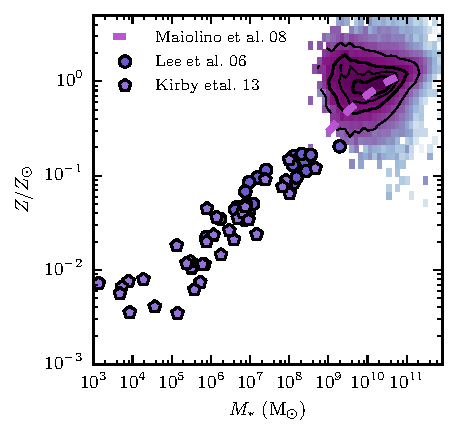
\includegraphics[scale=1.5]{fig/MsZ.pdf}}
\caption{Metallicities (in units of solar metallicity) of galaxies of different stellar mass. The histogram and contours show distribution of stellar metallicities of galaxies in the GAMA survey, while the magenta dashed lines shows the mean relation derived for the SDSS galaxies (\href{http://adsabs.harvard.edu/abs/2004ApJ...613..898T}{\citealt{tremonti_etal04}}) with with corrected calibration presented in \citet{maiolino_etal08}.
Blue circles show dwarf irregular galaxies from the study by \href{http://adsabs.harvard.edu/abs/2006ApJ...647..970L}{\citealt{lee_etal06}}, in which metallicities are derived from gas emission lines. Pentagons show nearby dwarf irregular and dwarf spheroidal galaxies in the compilation of \href{http://adsabs.harvard.edu/abs/2013ApJ...779..102K}{\citealt{kirby_etal13}}.  \label{fig:MsZ}}
\end{figure}

Figure \ref{fig:MsZ}  shows metallicities of stars in galaxies of different stellar masses from the smallest dwarf irregular  (from \href{http://adsabs.harvard.edu/abs/2006ApJ...647..970L}{\citealt{lee_etal06}}, and dwarf spheroidal \href{http://adsabs.harvard.edu/abs/2013ApJ...779..102K}{\citealt{kirby_etal13}}) galaxies to the largest galaxies probed by the GAMA survey. The figure also shows the relation derived for the SDSS galaxies (\href{http://adsabs.harvard.edu/abs/2004ApJ...613..898T}{\citealt{tremonti_etal04}}) with with corrected calibration presented in \href{http://adsabs.harvard.edu/abs/2008ApJ...681.1183K}{\citet{kewley_ellison08}} and \href{http://www.aanda.org/component/article?access=bibcode&bibcode=&bibcode=2008A%2526A...488..463MFUL}{\citet{maiolino_etal08}}.
Although there is significant scatter in metallicities at large $M_*$, overall galaxies follow a global trend of decreasing metallicity with decreasing stellar mass. Note that metallicities in the \href{http://adsabs.harvard.edu/abs/2006ApJ...647..970L}{\citet{lee_etal06}} study are measured from gas emission lines and thus reflect the metallicity of the gas. Those in the \href{http://adsabs.harvard.edu/abs/2013ApJ...779..102K}{\citealt{kirby_etal13}} study measure metallicities from stellar absorption lines and thus reflect metallicities of stars. Nevertheless, in the range of stellar masses where the two samples overlap, the metallicities are comparable. Although this does not have to be the case, in general, the Figure shows that for real galaxies we observe today the gas phase and stellar metallicities are similar. Both probes of gas and stellar metallicities are thus used to probe metallicity distributions in galaxies. 

The $M_*-Z$ relation shown in Figure \ref{fig:MsZ} and its evolution provide one of the key constraints on models of galaxy formation and their chemical evolution. 

Inside individual galaxies metallicity is not uniform. Stars exhibit a broad metallicity distribution. 
For example, in the Milky Way the lowest metallicity stars in the stellar halo have $Z/Z_\odot\sim 10^{-5}$ (e.g., see review by \href{http://adsabs.harvard.edu/abs/2015ARA%26A..53..631F}{\citealt{frebel_norris15}}), while most metal rich stars in the bulge have metallicities as high as $\sim 3Z_\odot$. Even in the smallest known galaxies, such as Segue 1 which has $M_*\approx 10^3\ M_\odot$, a spread of metallicities of $\sim 2$ orders of magnitude is obsvered (\href{http://adsabs.harvard.edu/abs/2011ApJ...733...46S}{\citealt{simon_etal11}}). The metallicity distributions are generally strongly peaked, however, and thus it does make sense to talk about characteristic metallicity of a galaxy.

In most disk galaxies there is also a weak trend of metallicity with radial distance (e.g., \href{http://adsabs.harvard.edu/abs/2014AJ....147..131P}{\citealt{pilyugin_etal14a}}, \href{http://adsabs.harvard.edu/abs/2015MNRAS.450.3254}{\citealt{pilyugin_etal15}}, \href{http://adsabs.harvard.edu/abs/2014A%26A...563A..49S}{\citealt{sanchez_etal14}}, \href{http://adsabs.harvard.edu/abs/2015MNRAS.454.3664B}{\citealt{bresolin_kennicutt15}}) which exhibits similar scaling when radii are expressed in units of the exponential scale lengths of the disk (\href{http://adsabs.harvard.edu/abs/2014A%26A...563A..49S}{\citealt{sanchez_etal14}}, \href{http://adsabs.harvard.edu/abs/2015MNRAS.454.3664B}{\citealt{bresolin_kennicutt15}}):
\begin{equation}
\frac{d\log_{10}(\mathrm{O/H})}{d(R/R_{\rm d})}=-0.102\pm 0.014\ \ \mathrm{[dex]},
\label{eq:universalZpro}
\end{equation}
where $\mathrm{O/H}$ is the abundance of oxygen atoms relative to hydrogen atoms. Given that $d(R/R_{\rm d})$ for galaxies with exponential profiles correspond to a given change in surface brightness, the radial gradient above can be recast as the change of metallicity with the change of surface brightness (\href{}{\citealt{pilyugin_etal14b}}, \href{http://adsabs.harvard.edu/abs/2015MNRAS.454.3664B}{\citealt{bresolin_kennicutt15}}): 
\begin{equation}
\Delta\log_{10}(\mathrm{O/H})=0.29\pm 0.1 \times \Delta\Sigma.
\label{eq:universalZpro}
\end{equation}
This, in turn, implies that there is a universal relation between surface brightness and metallicity in galaxies (\href{http://adsabs.harvard.edu/abs/1984MNRAS.211..507E}{\citealt{edmunds_pagel84}}, \href{http://adsabs.harvard.edu/abs/1995ApJ...444..610R}{\citealt{ryder95}}, \href{http://adsabs.harvard.edu/abs/2014AJ....148..134P}{\citealt{pilyugin_etal14b}}, \href{http://adsabs.harvard.edu/abs/2014A%26A...563A..49S}{\citealt{sanchez_etal14}}). 

%Although we know little about vertical abundance gradients in galaxies, such gradients are observed in the Milky Way. 

%-------------------------------
\section{Star formation}
\label{sec:sfoverview}
%-------------------------------

Regular star forming galaxies. Kennicutt-Schmidt relation. Quenched galaxies. Star bursts.

%--------------------------------------------
\section{Scaling relations of galaxies}
\label{sec:scalingrelns}
%--------------------------------------------

Above we have already seen that many properties of galaxies correlate with other properties. Such correlations indicate connection between different properties, which may provide clues about processes that governed galaxy formation. Some of these correlations are very tight and are thus a subject of particular attention. These are generally called scaling relations, although sometimes astronomers even call them ``laws.''  
Perhaps the most famous correlations of galaxies are the \href{http://adsabs.harvard.edu/abs/1977A%26A....54..661T}{\citet{tully_fisher77}} correlation between galaxy luminosity and the velocity width exhibited by its atomic hydrogen gas for disk galaxies and the qualitatively similar\href{http://adsabs.harvard.edu/abs/1976ApJ...204..668F}{\citet{faber_jackson76}}  relation between galaxy luminosity and stellar velocity dispersion for spheroidal galaxies. Correlations between more than pair of properties are also now routinely considered. The most famous of these is the fundamental plane of spheroidal galaxies (). 

\subsection{The Tully-Fisher relation of disk galaxies}

We have already briefly discussed the \href{http://www.scholarpedia.org/article/Tully-Fisher_relation}{Tully-Fisher relation} (TFR; \href{http://adsabs.harvard.edu/abs/1977A&A....54..661T}{\citealt{tully_fisher77}}) between galaxy luminosity and its rotation velocity in the context of galaxy scaling relations. Here we will discuss it in the context of gas content of galaxies by contrasting the standard stellar TFR with the so-called baryonic TFR between "baryon mass" of the galaxy, defined usually as a sum of stellar mass and mass of atomic hydrogen, and rotation velocity (\href{http://adsabs.harvard.edu/abs/2005ApJ...632..859M}{\citealt{mcgaugh05}}, \href{http://adsabs.harvard.edu/abs/2012AJ....143...40M}{\citealt{mcgaugh_etal12}}; \href{http://adsabs.harvard.edu/abs/2006ApJ...653..240G}{\citealt{geha_etal06}}). 

The baryonic TFR simply corrects the injustice of leaving the gas component of galaxies out of scaling relations which has clearly something to do with the equilibrium relations imposed by rotational equilibrium of disk galaxies, which should include all mass that contributes to acceleration against which rotational velocity stabilizes. 

Does it matter if gas mass is included? Let's find out. In what follows, I use the data from the \href{http://egg.astro.cornell.edu/alfalfa/}{ALFALFA 21 cm survey} to give the width of the 21 cm line containing half of the line flux, $W_{50}$, and $M_{\mathrm{HI}}$. The ALFALFA survey is cross-matched to the SDSS DR7 survey which gives redshift and optical photometry. I use the \href{http://adsabs.harvard.edu/abs/2015MNRAS.446.3943M}{\citet{meert_etal15}} photometric catalog\footnote{Available for download as a series of FITS tables \href{http://shalaowai.physics.upenn.edu/~ameert/fit_catalog/download/}{\underline{here}}.} derived from DR7 to provide magnitudes and probabilities for each galaxy to have a certain morphology derived using Bayesian analysis by \href{http://adsabs.harvard.edu/abs/2011A%26A...525A.157H}{\citealt{huertas_company_etal11}}).   

In the plot above, the blue dots are individual ALFALFA galaxies for which counterparts exist in the SDSS spectroscopic sample. The solid magenta line is the median $V_{\mathrm{rot}}$ at a given logarithmic bin of $L_r$, while the magenta dashed lines show the 16 and 84 percentiles of the distribution in each bin. 

The plot clearly shows a correlation, but it looks considerably messier and has larger scatter than what one usually sees in papers and textbook. The main reason for this is that here we deal with a large sample analyzed via a blind pipeline with measurements that carry relatively large errors compared to careful measurements for individual galaxies that usually go into construction of galaxy samples for the TFR. Nevertheless, there is a clear correlation close to a power law $L\propto V_{\mathrm{rot}}^{\alpha}$, where $\alpha\approx 4.3$, shown by the red dashed line. The scatter is $\sim 0.2-0.25$ dex in $V_{\mathrm{rot}}$ at a fixed $L_r$. This translates into a dex scatter in $L$. 
The real scatter for carefully constructed samples is about 5 times smaller than this. The slope, however, is similar. 

We can add mass of HI now to see what effect it has on the TFR by setting {\tt addHI} in the above script to True. Here I am just adding HI mass to stellar mass, which is obtained from $L_r$ using (u-r) color available in the ALFALFA catalog cross-matched to the SDSS and using linear relation from Table 7 of Bell et al. (2003). 
We will discuss what goes into such conversion in the next couple of lectures. For now this is just a convenient mapping. The addition of atomic gas has a pretty dramatic effect on the TFR, it changes the slope from $\approx 4.3$ to $\approx 3.3$ (dashed red line), which is much closer to the expectation for what such scaling should be from the models of halo structure for halos that form in Cold Dark Matter cosmology, which we will discuss later in the course.

\subsection{The Faber-Jackson relation of spheroidal galaxies}

Figure \ref{fig:faberjacksonsdss} shows the Faber-Jackson relation for the spheroidal galaxies in the SDSS sample. 
\href{http://adsabs.harvard.edu/abs/1976ApJ...204..668F}{\citet{faber_jackson76}} had a relatively sparse data and simply argued that relation between galaxy luminosity and $\sigma$ is power law of the form $L\propto \sigma^4$ and simply fitted for the normalization. The above plot shows spheroidal SDSS galaxies as the blue points, the median $\sigma$ at different $M_r$ as the magenta line and the $L\propto \sigma^4$ power law as the red dashed line. We can see that we can recover this power law for the bright SDSS galaxies. Velocity dispersion of galaxies fainter than $M_r\approx -20.5$ deviates low from this power law relation.\footnote{Does the $M_r\approx -20.5$ remind you of anything? Is this value of absolute magnitude notable for anything?} As we will see in this course, this will be a recurring theme. Similar deviation from power law occurs for the Tully-Fisher relation once faint dwarf galaxies are included. 

%We can look at a similar correlation for the disk galaxies, but results will not be particularly impressive. Any idea why? 
%Does it mean that the Tully-Fisher relation is not as good as the Faber-Jackson?

\subsection{The fundamental plane of spheroidal galaxies}

\href{http://adsabs.harvard.edu/abs/1987ApJ...313...42D}{\citet{dressler_etal87}} and \href{http://adsabs.harvard.edu/abs/1987ApJ...313...59D}{\citet{djorgovski_davis87}} discovered that spheroidal galaxies in the 3D space formed by the galaxy half-light radius, surface brightness, and velocity dispersion (or, equivalently, by luminosity, surface brightness, and velocity dispersion) are distributed along a manifold, which they dubbed the {\it fundamental plane.} The fundamental part is due to the low scatter perpendicular to the plane: these authors interpreted the combination of parameters that gives tight power law correlation between $R_{\rm eff}$ and the combination of the surface brightness and velocity dispersion as indicating the fundamental property that shapes sizes of spheroidal galaxies. 

Figure \ref{fig:fundplane} shows this plane in 3D for the SDSS main galaxy sample.  We can reproduce results of the classic  studies by \href{http://adsabs.harvard.edu/abs/1987ApJ...313...42D}{\citet{dressler_etal87}} and \href{http://adsabs.harvard.edu/abs/1987ApJ...313...59D}{\citet{djorgovski_davis87}} for a sample
of SDSS galaxies with criteria that should select early type galaxies, if we restrict the sample to $\sigma>100\ \mathrm{km/s}$. 
However, repeating the fit with lower thresholds for velocity dispersion results in the decrease of the power law slope in the $R_{\rm eff}-\sigma$ dependence. This illustrates that the actual manifold is not a plane but has some curvature to it, as was argued by \href{http://adsabs.harvard.edu/abs/2009MNRAS.394.1978H}{\citet{hyde_bernardi09}}. Such curvature can also be observed in the size-luminosity relation of galaxies, which previously was thought to be a power law. The reason people have talked about "planes" historically is because samples were dominated by massive galaxies. For the limited range of parameters the correlations could indeed be fit by power laws. The qualitative change came with analyses of large galaxy surveys during the last 15 years, when the correlations that were previously thought to be power laws turned out to be more complicated. These non-power law correlation have interesting implications for galaxy formation, which we will discuss later in the course. 

Both \href{http://adsabs.harvard.edu/abs/1987ApJ...313...42D}{\citet{dressler_etal87}} and \href{http://adsabs.harvard.edu/abs/1987ApJ...313...59D}{\citet{djorgovski_davis87}}  pointed out that the fact that low-scatter plane in the $R_{\rm eff}-\mu-\sigma$ exists provides a new independent distance indicator to spheroidal galaxies (although the fact that one can measure distances from projections of this plane has been pointed earlier; e.g., the title of the \href{http://adsabs.harvard.edu/abs/1977A&A....54..661T}{\citet{tully_fisher77}} paper is {\it "A new method of determining distances to galaxies"} --- i.e., the authors were more excited about measuring distances than about uncovering a tight correlation of disk galaxy properties per se.\footnote{Do you see how the fundamental plane or the Tully-Fisher correlation can be used to measure distances?}

%-------------------------------
\section{The Milky Way}
\label{sec:mwoverview}
%-------------------------------

Discuss key properties of the Milky Way in the context of the overall galaxy population. 
The Milky Way's $(g-r)$ color and $M_r$ absolute magnitude  are estimated to be $(g-r)_{\mathrm{MW}}=0.682^{+0.066}_{-0.056}$ and $M_{r,\rm MW}-5\log_{10}h=-21.0\pm 0.38$ \citet{licquia_etal15}. \citet{licquia_newman15} MW's star formation rate, stellar mass, and bulge-to-disk ratio. present a recent comprehensive review of the Milky Way properties.

Spiral structure and morphological type of the Milky Way (\href{http://adsabs.harvard.edu/abs/2011ARep...55..108E}{\citealt{efremov11}}. Milky Way is an early type barred Spiral 
of type around SBb. Scale length of the exponential disk is $R_{d,\rm MW}\approx 2.5\pm 0.5$ kpc (See \S 5.1.2 of \href{http://adsabs.harvard.edu/abs/2016arXiv160207702B}{\citealt{blandhawthorn_gerhard16}}); scale height changes with the Galacto-centric radius from $\approx 200$ pc in the inner regions to $\approx 300-400$ pc in the outer regions (See \S 5.1.1 of \href{http://adsabs.harvard.edu/abs/2016arXiv160207702B}{\citealt{blandhawthorn_gerhard16}}). Both the scale-height and scale-length vary with the age of stellar sub-population of the Milky Way disk (\href{http://adsabs.harvard.edu/abs/2013ApJ...779..115B}{\citealt{bovy_rix13}}).

As with many other structural properties, the information on the hot halo of the Milky Way is sparse. The state-of-the-art can be found in \href{http://adsabs.harvard.edu/abs/2013ApJ...770..118M}{\citet{miller_bregman13}} and \href{http://adsabs.harvard.edu/abs/2013MNRAS.433.2749G}{\citet{gatto_etal13}}.

%----------------------------------------------------------------------
\section{The Local Group and its local environment}
\label{sec:lgenv}
%---------------------------------------------------------------------



\section{Galaxy clustering and large-scale structure.}

Evidence for a ``supergalaxy'' \href{http://adsabs.harvard.edu/abs/1953AJ.....58...30D}{\citet{devaucouleurs53b}}. The very limited state of knowledge about large-scale structure circa 1970, and in particular the sizes and amplitudes of typical structures, is reflected in the paper by \href{http://adsabs.harvard.edu/abs/1970Sci...167.1203D}{\citet{devaucouleurs70}}, who argued forcefully that distribution of galaxies is highly non-uniform on large-scales. \href{http://adsabs.harvard.edu/abs/1978ApJ...222..784G}{\citet{gregory_thompson78}} presented the first modern-style redshift ``pie-slice'' diagram showing the main elements of the cosmic web as we now know it: clusters, filaments connecting them, and surrounding voids. Einasto's work in the late 1970s. The ``frothy'' structure of the web-like large-scale distribution of galaxies was further quantified in the surveys during the 1980s. 

Cosmic web, groups, clusters.

%----------------------------------------------------------------------------------------
\section{Evidence for dark matter in galaxies and galaxy clusters}
\label{sec:dmevidence}
%-----------------------------------------------------------------------------------------


%-------------------------------------------------------------------
\section{Additional reading}
%--------------------------------------------------------------------

For historical context, it is worth reading a brief three-page summary on Hubble's morphological classification in \href{http://adsabs.harvard.edu/abs/1926PASP...38..258H}{\citet{hubble26a}}, or you may check  the longer version
\href{http://adsabs.harvard.edu/abs/1926ApJ....64..321H}{\citet{hubble26}} from the same year. Recent review by \href{http://adsabs.harvard.edu/abs/2005ARA%26A..43..581S}{\citet{sandage05}} is an interesting window (in particular S 3 and S 4.2-4.4) into historical developments in galaxy morphological classification, as is the detailed paper by \citet{hart_berendzen71} about the history of how Hubble came up with his classification scheme and some of the rival scheme development.  

A good overview of galaxy properties at a level appropriate to both advanced undergraduate and graduate students can be found in S 1.1.1-1.1.2, 1.1.5, S 1.3-1.4 of ``Galaxies in the Universe'' book by \citet[][hereafter GS]{sparke_gallagher07}. 
Sections S 2.1, 2.2 (pp 25-36), 2.3.1, 2.3.2 (pp 37-45), 15.2.2 (pp 659-660) of the ``Galaxy formation and evolution'' book vt \citet*[][hereafter MvdBW]{mo_etal10}.
Up-to-date, research level discussion of galaxy properties can be found in S 2.1-2.4 and S 3.1-3.2 of review by \citet{blanton_moustakas09}.  A comprehensive recent review of the Milky Way properties and its place in the realm of galaxies is presented by \href{http://adsabs.harvard.edu/abs/2016arXiv160207702B}{\citet{blandhawthorn_gerhard16}}.

In depth historical overview of research on galaxy clusters from 1784 to 1983 (the year of George Abell's death) can be found in \href{http://adsabs.harvard.edu/abs/2000cucg.confE...1B}{\citet{biviano00}}.\footnote{Available as online version \href{https://ned.ipac.caltech.edu/level5/Biviano2/frames.html}{here}.} Current state of research into cluster formation is summarized in \href{http://adsabs.harvard.edu/abs/2012ARA%26A..50..353K}{\citet{kravtsov_borgani12}}. For a review of history of large-scale structure mapping, see \href{http://adsabs.harvard.edu/abs/2011arXiv1109.1268T}{\citet{thompson_gregory11}}.\footnote{Available as an online version \href{http://www.lairdthompson.net/void.html}{here}.}


%--------------------------------------------------------------------------------
\section{Ideas for exercises and explorations}
%--------------------------------------------------------------------------------

\begin{itemize}
\item[1.] Load the SDSS DR8 main galaxy catalog provided to you (see the example ipython notebook). Select a sub-sample of galaxies within a certain redshift range and apparent magnitude. Draw objects randomly from this sub-sample and display their images as shown in example python scripts. Classify these random draws morphologically using Hubble's classification scheme. Examine spectra of these objects and comment on the trends of spectral shapes with galaxy morphology. 
\item[2.] Try to construct the Hubble's tuning fork morphological diagram by such random drawings. Is it easy or difficult? What kind of galaxies are most common when you draw them randomly? 
\item[3.] Try to make cuts on other galaxy properties discussed in this chapter (e.g., luminosity, color, concentration, surface brightness). Is it easier to identify galaxies of particular morphological type with such cuts? With what galaxy properties does morphology correlate best?
What are the cuts in particular properties that allow you to select a given morphological type best?
\item[4.] The Milky Way half-light radius is $\approx 4.0\pm 0.5\ \mathrm{kpc}$. For example, \href{http://adsabs.harvard.edu/abs/2013ApJ...779..115B}{\citet{bovy_rix13}} estimate the scale-length of the Milky Way disk to be $R_d=2.15\pm 0.14$ kpc, while \href{http://adsabs.harvard.edu/abs/2011MNRAS.414.2446M}{\citet{mcmillan11}}  estimates $R_d\approx 3.1\pm 0.3$ kpc and half-light radius for exponential disk is $r_{50}\approx 1.68R_d$). Compute the $r$-band surface brightness of the Milky Way as it would be seen by an extragalactic observer (and show how you did it in intermediate steps). Plot the SDSS galaxies in the $\mu_r-M_r$ plot similar to the $\mu_r-m_r$ plot shown above and place your estimate for the Milky Way as a distinct point on the plot. Where is the Milky Way located relative to other disky galaxies in this diagram? 
\item[5.] Select ten (or more) galaxies nearest to the Milky Way in half-light radius, $M_r$, and color discussed in \S above and 
display a grid of thumbnail SDSS images of these objects (you can use example scripts in the ipython notebook that produced figures in this chapter). Examine images of these Milky Way analogues and describe their morphology. Do you notice any similarities? Compare morphologies of these analogues to typical morphologies of galaxies in the same region of the $(g-r)-M_r$ or $\mu_r-C_r$ diagram.
\end{itemize}


\appendix
%: Galaxies: overview of properties
%
%  Author:  Andrey Kravtsov
%  Date  :  March 2015
%
%


\chapter{Cosmological distances}
\label{sec:cosmodistances}

\noindent
{\it Reading:} \citet{hogg99}\\[2mm]
{\it More pedagogical reading:} Dodelson, "Modern cosmology" pp. 33-36, Mo, van den Bosch \& White ``Galaxy formation'', \S 3.1.1-3.1.4, 3.1.6\\[2mm]


Distances are one of the most difficult quantities to measure in astronomy. Although a number of good methods, which constitute rungs of the {\it distance ladder} (e.g., see review by \citealt{freedman_madore10}  and an older but methodologically excellent review by \citealt{jacoby_etal92}), exists, such measurements are difficult to do for large numbers of galaxies identified and observed in modern galaxy surveys, especially at distances $>50-100\ \mathrm{Mpc}$. Therefore, most commonly the Hubble law \citep{hubble29} is exploited to convert redshift into distance. Redshifts for such measurements are usually measured from spectra of galaxies of suitable resolution. However, now increasingly the {\it photometric redshifts\/} are measured from broad band photometry of galaxies. These are not particularly accurate individually but can be used to measure an accurate redshift of a galaxy cluster or for problems where high distance accuracy is not critical. 

A good collection of practical information about calculation of distances given a redshift of an object in expanding universe is provided by \citet[][see also Dodelson, "Modern cosmology" pp. 33-36]{hogg99}. What follows is a brief summary of the information relevant for galaxies that we will use lifted from that paper with minor modifications and addition of section on calculation of surface brightness by me. This info is for the standard $\Lambda$CDM cosmology, if you will ever need dark energy cosmology (with constant or varying $w$), you need S 2.1 and 2.2 in \citet{frieman_etal08}. 

Expansion of the universe leads locally to the Hubble law scaling between the recession velocity, $v$, implied by the redshift of spectral lines in spectrum, $z=\lambda_{\rm obs}/\lambda_{\rm emm}-1$, and distance, $d$: 

$$v=cz=H_0d,$$

where the Hubble constant $H_0$ is the proportionality constant. This constant has units of inverse time and its inverse can be used to define expansion time scale called {\it the Hubble time}:
\begin{equation}
t_{\rm H}\equiv\frac{1}{H_0}= 9.78\times10^9\,h^{-1}~{\rm yr}= 3.09\times10^{17}\,h^{-1}~{\rm s}
\end{equation}
The speed of light $c$ times the Hubble time is the {\it Hubble
distance} $D_{\rm H}$
\begin{equation}
D_{\rm H}\equiv\frac{c}{H_0}
= 3000\,h^{-1}~{\rm Mpc}= 9.26\times10^{25}\,h^{-1}~{\rm m}
\end{equation}

The mass density $\rho_{\rm m}$ of the Universe and the value of the
cosmological constant $\Lambda$ are dynamical properties of the
Universe, affecting the time evolution of the metric.  They can be
made into dimensionless density parameters $\Omega_{\rm M}$ and
$\Omega_{\Lambda}$ by normalizing by the {\it critical density of the universe} that would be required to make it spatially flat:
$$
\Omega_{\rm M}\equiv\frac{8\pi\,G\,\rho_0}{3\,H_0^2}
$$

$$
\Omega_{\Lambda}\equiv\frac{\Lambda\,c^2}{3\,H_0^2}
$$
(Peebles, 1993, pp. 310--313), where the subscripted zeroes indicate
that the quantities (which in general evolve with time) are to be
evaluated at the present epoch. The present-day value of the
critical density $\Omega=1$ corresponds to $7.5\times
10^{21}\,h^{-1}\,M_{\odot}\,D_{\mathrm{H}}^{-3}$, where $M_{\odot}$ is the
mass of the Sun. Taking Milky Way galaxy total mass $M\sim 10^{12}\ M_{\odot}$ as representative, this correspounds to roughly ten billion galaxies in the Hubble volume (the actual number is somewhat different as not all mass is in galaxies). 


A third density parameter $\Omega_k$
measures the ``curvature of space'' and can be defined by the relation
\begin{equation}
\Omega_{\rm M}+\Omega_{\Lambda}+\Omega_k= 1
\end{equation}
These parameters completely determine the geometry of the Universe if
it is homogeneous, isotropic, and matter-dominated, as will be assumed to be the case
in our study of galaxies.  

The best current estimates of these parameters from the CMB anisotropies, Baryonic Acoustic Oscillation feature in galaxy clustering, etc. can be found in this paper (although the precise values of some of the key parameters - e.g., $\Omega_{\rm m}$, $H_0$, and $\sigma_8$ are still under debate at the $\sim 5-10\%$ level, as different observational probes of these parameters are in tension with each other).

In terms of cosmography, the cosmological redshift is directly related
to the scale factor $a(t)$, or the ``size'' of the Universe.  For an
object at redshift $z$
\begin{equation}
1+z = \frac{a(t_{\rm o})}{a(t_{\rm e})}
\end{equation}
where $a(t_{\rm o})$ is the size of the Universe at the time the light
from the object is observed, and $a(t_{\rm e})$ is the size at the
time it was emitted.

There is usually a difference between an object's measured redshift $z_{\rm obs}$ and
its {\it cosmological redshift\/} $z_{\rm cos}$ due purely to the expansion of the universe. 
The difference is due to its (radial) {peculiar velocity\/} $v_{\rm pec}$; i.e,. we define the
cosmological redshift as that part of the redshift due solely to the
expansion of the Universe, or {\it Hubble flow.} The peculiar
velocity is related to the redshift difference by
\begin{equation}
v_{\rm pec} = c\,\frac{(z_{\rm obs}-z_{\rm cos})}{(1+z)}
\end{equation}
where it was assumed $v_{\rm pec}\ll c$. To estimate $v_{\rm pec}$ requires distance measurement independent of redshift, which is difficult but possible for limited number of galaxies. Thus, there are studies that estimate peculiar velocity field of galaxies locally. However, for most galaxies in the survey like the SDSS independent measurements are not available. From here on, we
assume $z=z_{\rm cos}$ when estimating distances. We should just keep in mind that in some cases we need to take into account the fact that redshift has two components to it, when we examine spatial distribution of galaxies in {\it redshift space}, as redshift derived distances will not correspond to the true spatial distances due to peculiar motions of galaxies relative to the uniformly expanding background. These motion lead to what's called {\it redshift space distorsions}. 

\section{Comoving distance (line-of-sight)}

A small {\em comoving distance\/} $\delta D_{\rm C}$ between two
nearby objects in the Universe is the distance between them which
remains constant with epoch if the two objects are moving with the
Hubble flow. 
The total line-of-sight comoving distance $D_{\rm C}$ from us to a
distant object is computed by integrating the infinitesimal $\delta
D_{\rm C}$ contributions between nearby events along the radial ray
from $z=0$ to the object:
\begin{equation}
D_{\rm C} = D_{\rm H}\,\int_0^z\frac{dz'}{E(z')}
\end{equation}
where $D_{\rm H}$ is the Hubble distance defined above and $E(z)$ is dimensionless Hubble parameter:
\begin{equation}
E(z)\equiv H(z)/H_0=\sqrt{\Omega_{\rm M}\,(1+z)^3+\Omega_k\,(1+z)^2+\Omega_{\Lambda}}
\end{equation}
Given that $dz=da$, $dz/E(z)$ is proportional to the
time-of-flight of a photon traveling across the redshift interval
$dz$, divided by the scale factor at that time.  Since the speed of
light is constant, this is a proper distance divided by the scale
factor, which is the definition of a comoving distance. 

The line-of-sight
comoving distance between two nearby events (ie, close in redshift or
distance) is the distance which we would measure locally between the
events today if those two points were locked into the Hubble flow.  It
is the correct distance measure for measuring aspects of large-scale
structure imprinted on the Hubble flow, eg, distances between
``walls.''

\section{Angular diameter distance}

The {\it angular diameter distance\/} $D_{\rm A}$ is defined as the
ratio of an object's physical transverse size to its angular size (in
radians).  It is used to convert angular separations in telescope
images into proper separations at the source.  It is famous for not
increasing indefinitely as $z\rightarrow\infty$; it turns over at
$z\sim 1$ and thereafter more distant objects actually appear larger
in angular size.  Angular diameter distance is related to the
transverse comoving distance by
\begin{equation}
D_{\rm A} = \frac{D_{\rm M}}{1+z}, 
\end{equation}

where 
\begin{equation}
D_{\rm M} = \left\{
\begin{array}{ll}
D_{\rm H}\,\frac{1}{\sqrt{\Omega_k}}\,\sinh\left[\sqrt{\Omega_k}\,D_{\rm C}/D_{\rm H}\right] & {\rm for}~\Omega_k>0 \\
D_{\rm C} & {\rm for}~\Omega_k=0 \\
D_{\rm H}\,\frac{1}{\sqrt{|\Omega_k|}}\,\sin\left[\sqrt{|\Omega_k|}\,D_{\rm C}/D_{\rm H}\right] & {\rm for}~\Omega_k<0
\end{array}
\right.
\end{equation}

 At high redshifts, the angular diameter
distance is such that 1 arcsec is on the order of 5 kpc.

\section{Luminosity distance}

The {\it luminosity distance} $D_{\rm L}$ is defined by the
relationship between bolometric (ie, integrated over all frequencies)
flux $S$ and bolometric luminosity $L$:
$$
D_{\rm L}\equiv \sqrt{\frac{L}{4\pi\,S}}
$$

It can be shown (Dodelson "Modern cosmology", S 2.2, pp. 34-36) that luminosity distance is related to the transverse comoving distance
and angular diameter distance by
$$
D_{\rm L} = (1+z)\,D_{\rm M} = (1+z)^2\,D_{\rm A}
$$

  The latter
relation implies that the surface brightness, $S$, of a
receding object of luminosity $L$ that subtends a given solid angle $\Omega$ will decrease with increasing redshift as $S=\Omega^{-1} L/D_{\rm L}^2\propto 1/[(1+z)^4D_{\rm A}^2]\propto 1/[(1+z)^4D^2]$, where $D^2=D_{\rm A}^2\Omega$ is proper area of the object. This is known as $(1+z)^4$ {\it cosmological surface brightness dimming\/} and is one of the main factors it makes it difficult to observe galaxies at high redshifts (even though their sizes do not change much). 


If the concern is not with bolometric quantities but rather with
differential flux $S_{\nu}$ and luminosity $L_{\nu}$, as is usually
the case in astronomy, then a correction, the {\it $k$-correction},
must be applied to the flux or luminosity because the redshifted
object is emitting flux in a different band than that in which you are
observing.  The k-correction depends on the spectrum of the object in
question, and is unnecessary only if the object has spectrum
$\nu\,L_{\nu}={\rm constant}$.  For any other spectrum the
differential flux $S_{\nu}$ is related to the differential luminosity
$L_{\nu}$ by
\begin{equation}
S_{\nu} = (1+z)\,\frac{L_{(1+z)\nu}}{L_{\nu}}\,\frac{L_{\nu}}{4\pi\,D_{\rm L}^2}
\end{equation}
where $z$ is the redshift, the ratio of luminosities equalizes the
difference in flux between the observed and emitted bands, and the
factor of $(1+z)$ accounts for the redshifting of the bandwidth.
Similarly, for differential flux per unit wavelength,
\begin{equation}
S_{\lambda} = \frac{1}{(1+z)}\,\frac{L_{\lambda/(1+z)}}{L_{\lambda}}\,
\frac{L_{\lambda}}{4\pi\,D_{\rm L}^2}.
\end{equation}

\section{Apparent and absolute magnitudes and $k$-correction}
\label{sec:mML}

The {\em apparent magnitude\/} $m$ of an astronomical source in a
photometric bandpass is defined to be the ratio of the apparent flux
of that source to the apparent flux of the bright reference stars through
that bandpass.  The
{\em distance modulus\/} $DM$ is defined by
\begin{equation}
DM\equiv 5\,\log \left(\frac{D_{\rm L}}{10~{\rm pc}}\right)
\end{equation}
because it is the magnitude difference between an object's observed
bolometric flux and what it would be if it were at $10~{\rm pc}$ (this
was once thought to be the distance to Vega which was the most commonly used standard star until recently).  

The absolute magnitude $M$ is the
astronomer's measure of luminosity, defined to be the apparent
magnitude the object in question would have if it were at 10~pc, so
\begin{equation}
m=M+DM+K(z)
\label{eq:mM}
\end{equation}
where $K$ is the so called {\it $k$-correction}:
\begin{equation}
K(\lambda_0) = 2.5\,\log \left[(1+z)\,\frac{\int_0^{\infty} f(\lambda_0) S(\lambda)d\lambda}{\int_0^\infty f[\lambda_0/(1+z)]S(\lambda)d\lambda}\right],
\label{eq:kcorr}
\end{equation}
where $\lambda_0$ is the wavelength of the filter at $z_0$ to which we would like to correct the magnitudes (\href{http://adsabs.harvard.edu/abs/1968ApJ...154...21O}{\citealt{oke_sandage68}},  see \S 4 in \href{http://adsabs.harvard.edu/abs/2007AJ....133..734B}{\citealt{blanton_roweis07}} for a more complete treatment).

Given the galaxy absolute magnitude $M_{\rm f}$ estimated for a given filter using equations above, we can compute galaxy luminosity in units of solar luminosity in the same filter as 
\begin{equation}
L_{\rm f} = 10^{0.4(M_{\odot,\rm f}-M_{\rm f})},
\label{eq:LMf}
\end{equation}
where $M_{\odot,\rm f}$ is the absolute magnitude of the Sun in the same band (see, e.g., eq. 14 in \href{http://adsabs.harvard.edu/abs/2003ApJ...592..819B}{\citealt{blanton_etal03}} for the SDSS bands and \href{http://mips.as.arizona.edu/~cnaw/sun.html}{here} for many other commonly used bands).

\section{Surface brightness}
\label{sec:surface_brightness}
If a given patch in a galaxy at redshift $z$ has the surface brightness $S_b$ in some band $b$ in units of $L_{\odot,b}\,\mathrm{pc}^{-2}$ (where $L_{\odot,b}$ is Sun's luminosity in the same band) in the small angle approximation the luminosity of the patch corresponding to the solid angle of $1\ \mathrm{arcsec}^2$ will be $L_1=S_b\,\Omega_1 D_{\rm A}^2(z)$, where $\Omega_1=2.35044\times 10^{-11}$ is the solid angle in steradians corresponding to one square arcsecond. 

The absolute magnitude of the galaxy will be 
\begin{equation}
M_b=M_{\odot,b}-2.5\log_{10}\frac{L_1}{L_{\odot,b}}=M_{\odot,b}-2.5\log_{10}S_b-2.5\log_{10}\Omega_1-5\log_{10}D_{\rm A}(z)
\end{equation}
The apparent magnitude of such square arcsecond patch will then be
\begin{equation}
\mu_b = M_b+5\log_{10}D_{\rm L} - 5=
M_{\odot,b}-2.5\log_{10}S_b-2.5\log_{10}\Omega_1-5+5\log_{10}\left(D_{\rm L}/D_{\rm A}
\right)
\end{equation}
where $D_{\rm L}=D_{\rm A}(1+z)^2$  is luminosity distance. Substituting this and the value of $\Omega_1$ into the equation above gives expression for surface brightness in the same band $b$ in magnitudes per arcsecond square:
\begin{equation}
\mu_b = 21.5721 + M_{\odot,b}-2.5\log_{10}S_b+10\log_{10}(1+z),
\label{eq:musb}
\end{equation}
where the last term represents the $(1+z)^4$ cosmological dimming. To use this equation we need to know Sun's absolute magnitude in different bands. You can find a useful compilation of these \underline{\href{http://www.ucolick.org/~cnaw/sun.html}{here}}.

%-----------------------------
\section{$h$-scalings}
\label{sec:hscalings}
%-----------------------------

Astronomical literature contains ubiquitous $h$-scalings when specific values of different quantities, such as luminosities, are quoted (see, for example, Figure \ref{fig:lfmagdefs} in Ch. \ref{ch:overview}). The main reasons for scaling distance-dependent quantities with $h$ are that 1) distances for most galaxies are determined from their redshift and using cosmological distance-redshift relation involving the Hubble constant, $d\propto h^{-1}$, and 2) the fact that for a long time the Hubble constant was uncertain by a factor of two. Explicit scalings were thus meant to allow easy rescaling of quantities to a specific value of the Hubble constant. Although the rationale is much weakened by a much more accurate modern knowledge of $H_0$, the explicit scalings persist as uncertainty of $\sim 5-10\%$ in $h$ is still present and this uncertainty is  substantial for some quantities. 

Here I review the main origin of such scalings for quantities for which they are most commonly quoted. 
Luminosities of galaxies depend on measured flux, $f$, and inverse square of the distance, as discussed above. 
Thus, the $h$-scaling of luminosity is $L\propto f d^{2}\propto h^{-2}$, while the absolute magnitude scales as $M\propto \ldots +5\log_{10}h$, so that absolute magnitudes are commonly plotted in units of $\mathrm{mag}-5\log_{10}h$. 

Physical sizes or observables defined within a given aperture scale with $h$ 
because distances are used to convert observed angular scale, $\theta$, to physical
size within which an ``observable'' is defined, 
$R=\theta d_A(z)\propto \theta h^{-1}$.
Thus, if the total mass $M$ of a galaxy or galaxy cluster is measured using the hydrostatic equilibrium equation and measurement of the temperature of velocity dispersion profile, we have $M_{\rm HE}\propto \sigma R\ \mathrm{or}\ \propto T R\propto d_A\propto h^{-1}$. The same scaling is expected for the mass derived from the weak lensing shear profile measurements. 

If the gas mass is measured from the X-ray flux from a volume
$V\propto R^3\propto \theta^3d_A^3$, which scales as $f=L_{\rm X}/(4\pi
d_L^2)\propto \rho_{\rm gas}^2 V/d_L^2\propto M_{\rm gas}^2/(Vd_L^2)\propto
M_{\rm gas}^2/(\theta d_L^2 d_A^3)$ and where $f$ and $\theta$ are
observables, gas mass then scales with distance as $M_{\rm gas}\propto d_L
d_A^{3/2}\propto h^{5/2}$. This dependence can be exploited to
constrain cosmological parameters, as in the case of X--ray
measurements of gas fractions in clusters.  

%------------------------------------
\section{Comoving volume}
\label{sec:Vcom}
%------------------------------------

The {\it comoving volume\/} $V_{\rm C}$ is the volume measure in which
number densities of non-evolving objects locked into Hubble flow are
constant with redshift.  It is the proper volume times three factors
of the relative scale factor now to then, or $(1+z)^3.$

Given that the
derivative of comoving distance with redshift is $1/E(z)$, the angular diameter distance converts a solid angle
$d\Omega$ into a proper area, and two factors of $(1+z)$ convert a
proper area into a comoving area, the comoving volume element in solid
angle $d\Omega$ and redshift interval $dz$ is
\begin{equation}
dV_{\rm C}= D_{\rm H}\,\frac{(1+z)^2\,D_{\rm A}^2}{E(z)}\,d\Omega\,dz
\end{equation}

The integral of the comoving volume element
from the present to redshift $z$ gives the total comoving volume,
all-sky, out to redshift $z$
\begin{equation}
V_{\rm C} = \left\{
\begin{array}{ll}
  \left(\frac{4\pi\,D_{\rm H}^3}{2\,\Omega_k}\right)\,
  \left[\frac{D_{\rm M}}{D_{\rm H}}\,
  \sqrt{1+\Omega_k\,\frac{D_{\rm M}^2}{D_{\rm H}^2}}
  -\frac{1}{\sqrt{|\Omega_k|}}\,
  {\rm arcsinh}\left(\sqrt{|\Omega_k|}\,\frac{D_{\rm M}}{D_{\rm H}}\right)\right]
  & {\rm for}~\Omega_k>0 \\
  \frac{4\pi}{3}\,D_{\rm M}^3
  & {\rm for}~\Omega_k=0 \\
  \left(\frac{4\pi\,D_{\rm H}^3}{2\,\Omega_k}\right)\,
  \left[\frac{D_{\rm M}}{D_{\rm H}}\,
  \sqrt{1+\Omega_k\,\frac{D_{\rm M}^2}{D_{\rm H}^2}}
  -\frac{1}{\sqrt{|\Omega_k|}}\,
  {\rm arcsin}\left(\sqrt{|\Omega_k|}\,\frac{D_{\rm M}}{D_{\rm H}}\right)\right]
  & {\rm for}~\Omega_k<0
\end{array}
\right.
\end{equation}
\citet{carroll_etal92}. The comoving volume element and its
integral are both used frequently in predicting number counts or
luminosity densities.

\section{Lookback time}

The {\it lookback time\/} $t_{\rm L}$ to an object is the difference
between the age $t_{\rm o}$ of the Universe now (at observation) and
the age $t_{\rm e}$ of the Universe at the time the photons were
emitted (according to the object).  It is used to predict properties
of high-redshift objects with evolutionary models, such as passive
stellar evolution for galaxies.  Recall that $E(z)$ is the time
derivative of the logarithm of the scale factor $a(t)$; the scale
factor is proportional to $(1+z)$, so the product $(1+z)\,E(z)$ is
proportional to the derivative of $z$ with respect to the lookback
time, or
\begin{equation}
t_{\rm L} = t_{\rm H}\,\int_0^z \frac{dz'}{(1+z')\,E(z')}
\end{equation}
\citet[e.g.,][pp 313-315]{peebles93} and \citet[][pp 52-56]{kolb_turner90} give some
analytic solutions to this equation, but they are concerned with the
age $t(z)$, so they integrate from $z$ to $\infty$). 



\chapterimage{python_xkcd2.PNG} 

%-----------------------------------
\chapter{{\tt python} info}
%-----------------------------------

%------------------------------------------
\section{{\tt Ipython} notebooks}
%-----------------------------------------

I will be using IPython Notebooks to supplement whatever I show in class. These can be viewed, edited, and produced with IDE editors of the main python distros (Enthought or Anaconda).\footnote{Note that you can request a free Enthought academic license which will allow you to get distribution with many add-ons and libraries}  Also, I recommend the {\tt PyCharm} IDE environment\footnote{\href{https://www.jetbrains.com/pycharm/}{https://www.jetbrains.com/pycharm/}} for code development, which can be obtained free for academic users. 

If you don't have a python distribution installed on your machine, please do so asap. The rationale for using Notebooks can be found \href{http://pgbovine.net/ipython-notebook-first-impressions.htm}{\underline{here}} - it simplifies work flow and closely connects plots that we will be discussing with the code that produces them. You can use these codes as a starting point for your own experimentation with data or calculations. 

To run examples presented here, you will need to install python (Enthought or Anaconda distributions) with standard libraries (matplotlib, numpy, scipy, etc). In addition, make sure you have pyfits installed for reading FITS files. The FITS file with the SDSS data will be distributed (also I will distribute SQL script that was used to query SDSS DR8 to produce it). 

%------------------------------------------
\section{{\tt colossus}}
%-----------------------------------------

For cosmological functions, such as distances, we will use the \href{http://www.benediktdiemer.com/code/}{{\tt colossus} package} written by Benedikt Diemer. We will also use it when we explore properties of dark matter halo profiles. You can install it by
\begin{lstlisting}
pip install https://bitbucket.org/bdiemer/colossus/get/tip.tar.gz
or
easy_install https://bitbucket.org/bdiemer/colossus/get/tip.tar.gz
\end{lstlisting}

%------------------------------------------
\section{{\tt AstroML}}
%-----------------------------------------

We will also use some functions and examples from the \href{https://pypi.python.org/pypi/astroML/}{AstroML python library}, especially when we will come to more sophisticated analyses, such as clustering. This library was developed to support the book \href{http://press.princeton.edu/titles/10159.html}{''Statistics, Data Mining, and Machine Learning in Astronomy''} \citep{ivezic_etal13}. The book itself is not needed for this course, although I will draw on it in parts of the course. It is very good though and I highly recommend to get and study it (it is not available in our library yet, unfortunately, but many of your fellow graduate students already have it). In any case, all of the figures from the book and the python code used to produce them is available online \href{http://www.astroml.org/book_figures/index.html}{here}. 

\chapterimage{sdss_data_banner.png} 
%-----------------------------------
\chapter{Data access info}
%-----------------------------------

%-------------------------------------------------------
\section{SDSS DR8 main galaxy sample}
%-------------------------------------------------------
 For many exercises here and subsequent lectures we will be using SDSS data. The binary FITS file used in the explorations below can be downloaded \href{http://astro.uchicago.edu/~andrey/classes/a304s15/data/sdss_dr8/SDSSspecgalsDR8.fit}{here} (it is 165 Mb). It was produced at the SDSS \href{http://skyserver.sdss.org/CasJobs/}{CasJobs server} where time-intensive SQL queries can be submitted. The FITS file used below is large because it includes a number of properties that will be useful in our explorations and because it selects almost all low-$z$ galaxies from the SDSS (called the main galaxy sample, to differentiate from the quasar and LRG samples). 

The SQL script used to produce the FITS file below can be found \href{http://astro.uchicago.edu/~andrey/classes/a304s15/data/sdss_dr8/README.txt}{here}. Description of various entries for SDSS objects classified as GALAXY in DR8 can be found \href{http://skyserver.sdss.org/dr8/en/help/browser/browser.asp?n=Galaxy&t=U}{here}, for STAR objects see \href{http://skyserver.sdss.org/dr8/en/help/browser/description.asp?n=Star&t=V}{here}, while QSOs are \href{}{here}. If you have not queried SDSS data base yet, I encourage you to use this example, to create your own queries for particular properties. 

\subsection{Petrosian magnitudes and sizes}
\label{sec:petromagsize}

In \S \ref{sec:apermags} we discussed the \citet{petrosian76} definition of the galaxy magnitude and size and the specific implementation of this definition in the SDSS  (see \href{http://skyserver.sdss.org/dr1/en/help/docs/algorithm.asp?key=mag_petro}{here} for more details) computes the following function as a function of angular radius, $R$, from galaxy center:
\begin{equation}
\eta(R)\equiv\frac{\int_{0.8R}^{1.25R}dR^\prime 2\pi R^\prime \Sigma(R^\prime)/[\pi(1.25^2-0.8^2)R^2]}{\int^R_02\pi R^\prime \Sigma(R^\prime) dR^\prime/(\pi R^{2})}
\label{eq:Rpetro}
\end{equation}
where $\Sigma(r)$ is the surface brightness profile. The {\it Petrosian radius,\/} $R_{\rm P}$, is then defined by the SDSS pipeline as the radius where $\eta(R_{\rm P})=0.2$.
Galaxy flux is then measured within some multiple of $R_{\rm P}$:
\begin{equation}
F_{\rm P}\equiv \int^{N_{\rm P}R_{\rm P}}_0 2\pi R^\prime I(R^\prime)dR^\prime
\label{eq:fPetro}
\end{equation}
The aperture $2R_{\rm P}$ used in the SDSS measurements. 

The choices for $\eta$ and $N_{\rm P}$ are heuristic. It  is argued to be large enough to contain nearly all of the flux for many galaxies (in particular late type galaxies described by the exponential profile), but small enough that the sky noise is sub-dominant in $F_{\rm P}$. In this case, even substantial errors in $R_{\rm P}$ cause only small errors in the Petrosian flux (typical statistical errors near the spectroscopic flux limit of $r \sim 17.7$ are $< 5\%$). The 
 main draw of the Petrosian's definition, however, is that the fraction of recovered light is robust and depend  only weakly on the galaxy axis ratio or size variation due to worse seeing or greater distance \href{http://adsabs.harvard.edu/abs/2001AJ....121.2358B}{\citep[e.g.,][]{blanton_etal01}}. 

The Petrosian radius in each band is the parameter {\tt petroRad} in the database with the subscript corresponding to 
particular filter (e.g., for $r$-band, {\tt petroRad\_r}) and the Petrosian magnitude in each band (calculated using only petroRad for the $r$ band) is the parameter petroMag (e.g., for $r$-band, {\tt petroMag\_r}) . 

SDSS main galaxy sample  also provides radii enclosing 50\% and 90\% of the total light of the Petrosian magnitude (e.g., {\tt petroR50\_r} and {\tt petroR90\_r} for the $r$ band). 

\subsection{cmodel magnitudes}
\label{sec:cmodelmag}
%\appendix{Practical info on accessing various data sets}
\chapterimage{banner_bookshelf.jpg} 
\printbibliography

%----------------------------------------------------------------------------------------
%	INDEX
%----------------------------------------------------------------------------------------

%\cleardoublepage
%\phantomsection
%\setlength{\columnsep}{0.75cm}
%\addcontentsline{toc}{chapter}{\textcolor{ocre}{Index}}
%\printindex

%----------------------------------------------------------------------------------------

\end{document}

%------------------------------------------------

\section{Figure}\index{Figure}

\begin{figure}[h]
\centering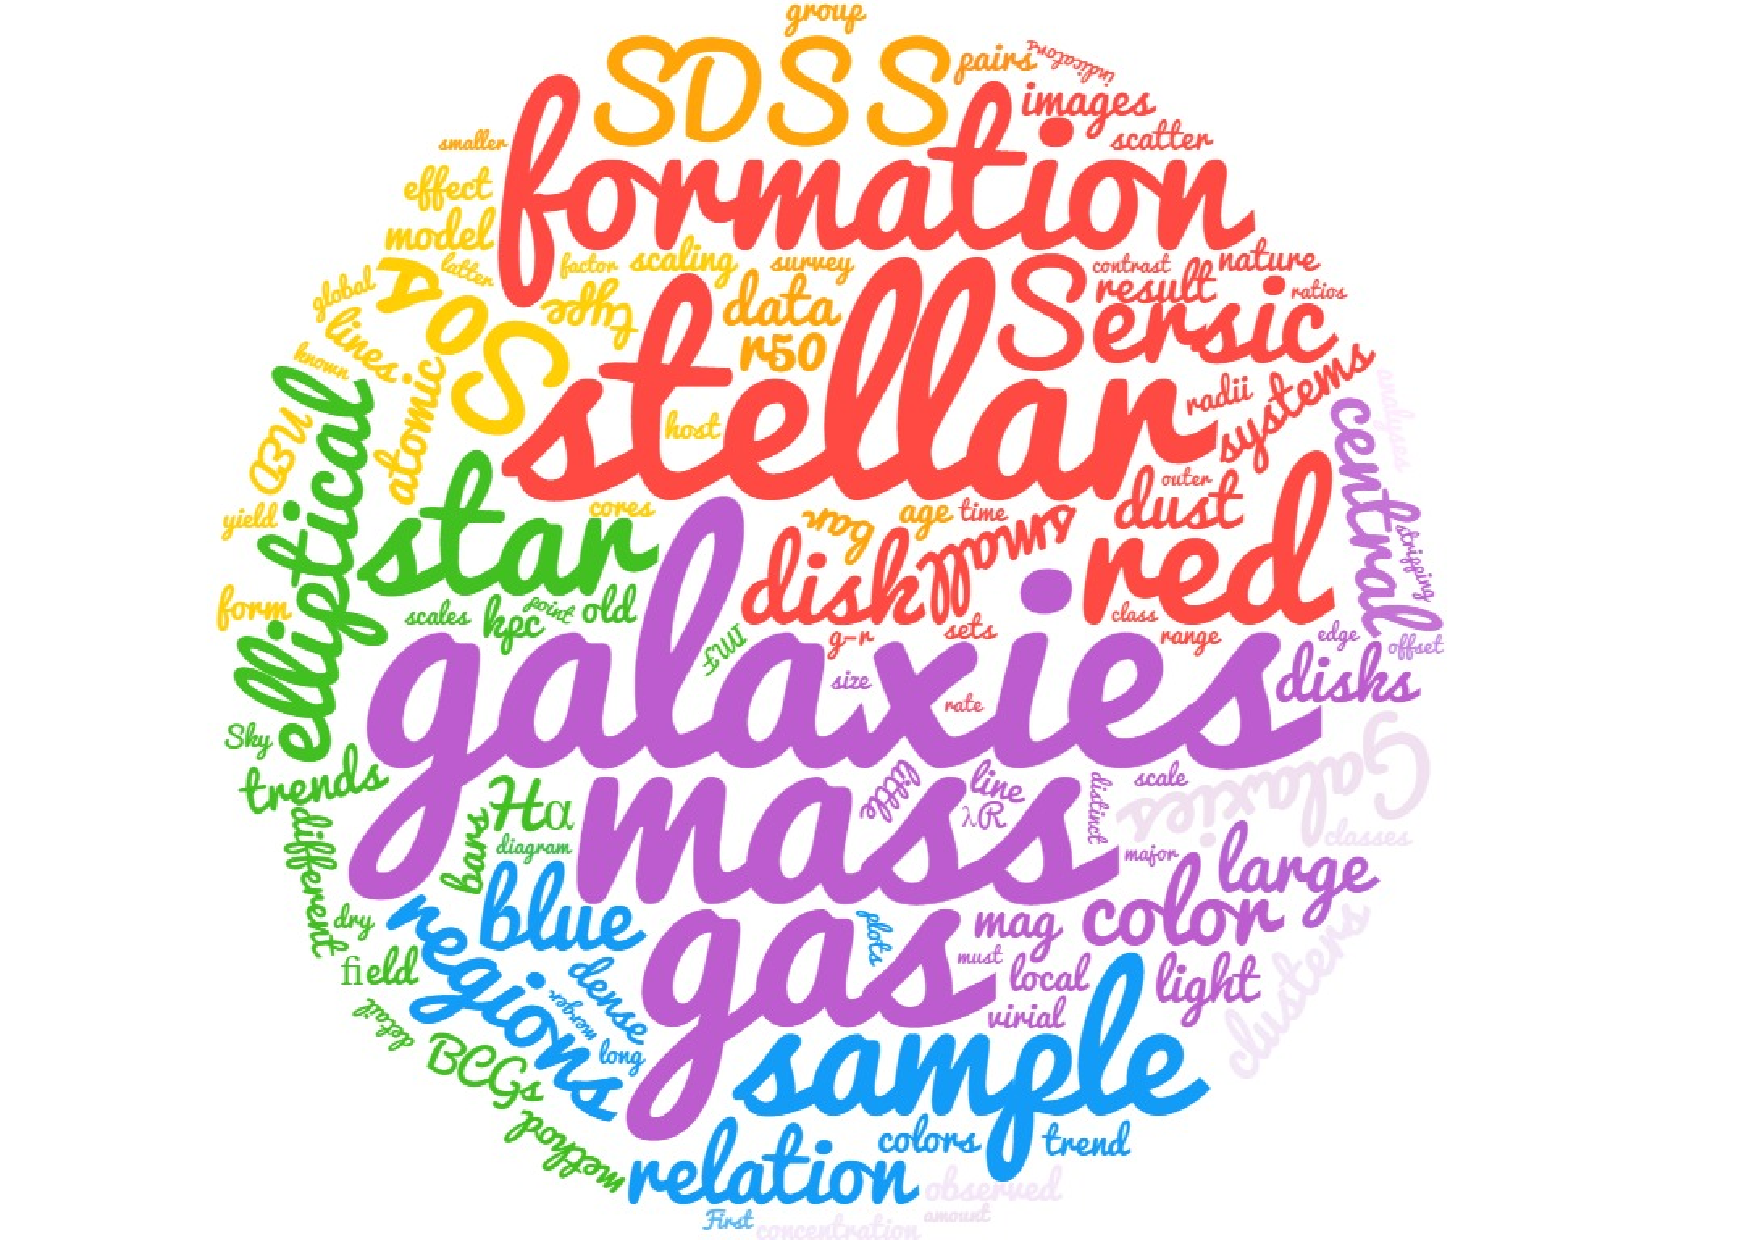
\includegraphics[scale=0.5]{blanton_moustakas_wordcloud.pdf}
\caption{Figure caption}
\end{figure}


\begin{figure}[ht]
\includemedia[
label=LG,
width=0.5\linewidth,height=0.5\linewidth,
activate=pageopen,
3Dtoolbar, 3Dmenu,
3Dviews=dice.vws,
]{}{fig/LG3d.u3d}
\end{figure}
\end{document}
